%
% $RCSfile: paper.tex,v $
%
% Copyright (c) 2001-2004. Christian Heller. All rights reserved.
%
% No copying, altering, distribution or any other actions concerning this
% document, except after explicit permission by the author!
% At some later point in time, this document is planned to be put under
% the GNU FDL license. For now, _everything_ is _restricted_ by the author.
%
% http://www.cybop.net
% - Cybernetics Oriented Programming -
%
% http://www.resmedicinae.org
% - Information in Medicine -
%
% @author Christian Heller <christian.heller@tuxtax.de>
%

%
% The document class specifying the type of document.
%
\documentclass[a4paper,10pt]{llncs}

%
% The usepackages for document class.
%

% Paper format and font.
\usepackage{a4,times,helvet}

% Graphics.
\usepackage{graphicx}

%
% The space settings for edges (left, top, right, bottom).
%
\setlength{\hoffset}{-1,3in}
\setlength{\voffset}{-1in}
\setlength{\oddsidemargin}{3,5cm}
\setlength{\topmargin}{1,3cm}
%\setlength{\headwidth}{16,5cm}
\setlength{\headheight}{0cm}
\setlength{\textwidth}{16,5cm}
\setlength{\textheight}{23,2cm}

%
% The hyphenation list.
%
%
% $RCSfile: hyphenation.tex,v $
%
% Copyright (c) 2002-2007. Christian Heller. All rights reserved.
%
% Permission is granted to copy, distribute and/or modify this document
% under the terms of the GNU Free Documentation License, Version 1.1 or
% any later version published by the Free Software Foundation; with no
% Invariant Sections, with no Front-Cover Texts and with no Back-Cover
% Texts. A copy of the license is included in the section entitled
% "GNU Free Documentation License".
%
% http://www.cybop.net
% - Cybernetics Oriented Programming -
%
% Version: $Revision: 1.2 $ $Date: 2007-08-01 13:59:00 $ $Author: christian $
% Authors: Christian Heller <christian.heller@tuxtax.de>
%

\hyphenation{abs-trac-tion}
\hyphenation{ac-tu-ally}
\hyphenation{ana-lyst}
\hyphenation{ana-ly-sis}
\hyphenation{an-cient}
\hyphenation{ap-pli-ca-tion}
\hyphenation{aris-to-tle}
\hyphenation{at-tri-bute}
\hyphenation{be-ing}
\hyphenation{ca-te-go-ri-za-tion}
\hyphenation{client}
\hyphenation{com-po-nen-ti-za-tion}
\hyphenation{com-pu-ter}
\hyphenation{con-fi-gure}
\hyphenation{con-nec-ted}
\hyphenation{cy-ber-ne-tics}
\hyphenation{cyboi}
\hyphenation{cybol}
\hyphenation{cybop}
\hyphenation{des-cribed}
\hyphenation{de-sign}
\hyphenation{de-ve-lop-ment}
\hyphenation{dis-crete}
\hyphenation{di-vide}
\hyphenation{do-main}
\hyphenation{dy-na-mic}
\hyphenation{eli-mi-nate}
\hyphenation{eli-mi-nates}
\hyphenation{eli-mi-na-tion}
\hyphenation{en-gi-nee-ring}
\hyphenation{en-vi-ron-ment}
\hyphenation{ex-pert}
\hyphenation{fi-gure}
\hyphenation{fle-xi-bi-li-sie-rung}
\hyphenation{fun-da-men-tal}
\hyphenation{hard-ware}
\hyphenation{hu-man}
\hyphenation{im-ple-men-ta-tion}
\hyphenation{in-he-rit}
\hyphenation{in-he-ri-tance}
\hyphenation{in-ter-pre-ter}
\hyphenation{java}
\hyphenation{know-ledge}
\hyphenation{lan-guage}
\hyphenation{li-ving}
\hyphenation{lo-gi-cal}
\hyphenation{ma-na-ge-ment}
\hyphenation{mea-ning-ful}
\hyphenation{me-cha-nism}
\hyphenation{me-mo-ry}
\hyphenation{me-thod}
\hyphenation{me-thods}
\hyphenation{mo-del-ling}
\hyphenation{na-ture}
\hyphenation{net-work}
\hyphenation{neu-ral}
\hyphenation{neu-ron}
\hyphenation{ne-ver-en-ding-ly}
\hyphenation{open}
\hyphenation{operating}
\hyphenation{ori-en-ted}
\hyphenation{over-come}
\hyphenation{par-ti-cu-lar}
\hyphenation{prin-ci-ple}
\hyphenation{pro-ba-bi-lis-tic}
\hyphenation{pro-ble-ma-tic}
\hyphenation{pro-gram-ming}
\hyphenation{res-pon-sible}
\hyphenation{re-u-sa-bi-li-ty}
\hyphenation{sci-ence}
\hyphenation{server}
\hyphenation{si-mi-lar}
\hyphenation{soft-ware}
\hyphenation{source}
\hyphenation{spe-cia-li-za-tion}
\hyphenation{spe-ci-fied}
\hyphenation{sta-tic}
\hyphenation{sta-ti-cally}
\hyphenation{sto-chas-tic}
\hyphenation{stone-on-stone}
\hyphenation{struc-ture}
\hyphenation{strug-gling}
\hyphenation{subs-ti-tu-ting}
\hyphenation{su-per-flu-ous}
\hyphenation{sup-ply-ing}
\hyphenation{sys-tem}
\hyphenation{taeu-schungs-ver-such}
\hyphenation{temp-lates}
\hyphenation{tes-ting}
\hyphenation{thin-king}
\hyphenation{un-en-li-vened}
\hyphenation{un-sa-tis-fy-ing}
\hyphenation{va-ry-ing}
\hyphenation{weigh-ted}
\hyphenation{zu-kunfts-si-che-re}


%
% This document is a scientific paper to be handed in for a conference.
%
% @version $Revision: 1.1 $ $Date: 2003-10-08 12:40:03 $ $Author: christian $
% @author Christian Heller <christian.heller@tuxtax.de>
% @author Christian Heller <christian.heller@tu-ilmenau.de>
%
\begin{document}
    \twocolumn
    \title{Flexible Software Architectures for Presentation Layers demonstrated on Medical Documentation with Episodes and Inclusion of Topological Report}
\author{Jens Bohl \(<\)info@jens-bohl.de\(>\)\\
Torsten Kunze \(<\)zone3@gmx.de\(>\)\\
Christian Heller \(<\)christian.heller@tu-ilmenau.de\(>\)\\
Ilka Philippow \(<\)ilka.philippow@tu-ilmenau.de\(>\)}
\institute{
Technical University of Ilmenau\\
Faculty for Computer Science and Automation\\
Institute for Theoretical and Technical Informatics\\
PF 100565, Max-Planck-Ring 14, 98693 Ilmenau, Germany\\
http://www.tu-ilmenau.de, fon: +49-(0)3677-69-1230, fax: +49-(0)3677-69-1220}
\maketitle

    \maketitle
    %
% $RCSfile: abstract.tex,v $
%
% Copyright (c) 2001-2004. Christian Heller. All rights reserved.
%
% No copying, altering, distribution or any other actions concerning this
% document, except after explicit permission by the author!
% At some later point in time, this document is planned to be put under
% the GNU FDL license. For now, _everything_ is _restricted_ by the author.
%
% http://www.cybop.net
% - Cybernetics Oriented Programming -
%
% http://www.resmedicinae.org
% - Information in Medicine -
%
% @author Christian Heller <christian.heller@tuxtax.de>
%

\begin{abstract}
This article reports about an ongoing research investigating the possibilities
for applying inter-disciplinary concepts to software system design. The new
resulting programming philosophy is based on firstly, a distinction of statics
and dynamics, secondly a knowledge schema structuring models and their meta
information hierarchically, and thirdly the separation of state- and logic
knowledge. It solves many of the problems existing in classical programming
paradigms and languages and may have the potential to replace these in the long
run.\\
\textbf{Keywords:} Knowledge Abstraction, Cybernetics Oriented Programming,
CYBOP, Software Design
\end{abstract}

    %
% $RCSfile: introduction.tex,v $
%
% Copyright (c) 2002-2007. Christian Heller. All rights reserved.
%
% Permission is granted to copy, distribute and/or modify this document
% under the terms of the GNU Free Documentation License, Version 1.1 or
% any later version published by the Free Software Foundation; with no
% Invariant Sections, with no Front-Cover Texts and with no Back-Cover
% Texts. A copy of the license is included in the section entitled
% "GNU Free Documentation License".
%
% http://www.cybop.net
% - Cybernetics Oriented Programming -
%
% Version: $Revision: 1.1 $ $Date: 2007-07-17 20:02:36 $ $Author: christian $
% Authors: Christian Heller <christian.heller@tuxtax.de>
%

\chapter{Introduction}
\label{introduction_heading}
\index{Introduction}

This is just a test \cite{zimmermann} citation.

%
% $RCSfile: terminology.tex,v $
%
% Copyright (C) 2002-2008. Christian Heller.
%
% Permission is granted to copy, distribute and/or modify this document
% under the terms of the GNU Free Documentation License, Version 1.1 or
% any later version published by the Free Software Foundation; with no
% Invariant Sections, with no Front-Cover Texts and with no Back-Cover
% Texts. A copy of the license is included in the section entitled
% "GNU Free Documentation License".
%
% http://www.cybop.net
% - Cybernetics Oriented Programming -
%
% http://www.resmedicinae.org
% - Information in Medicine -
%
% Version: $Revision: 1.1 $ $Date: 2008-08-19 20:41:09 $ $Author: christian $
% Authors: Christian Heller <christian.heller@tuxtax.de>
%

\subsection{Terminology}
\label{terminology_heading}
\index{Terminology}
\index{Lexicon}
\index{Vocabulary}
\index{Nomenclature}
\index{Hierarchy}
\index{Semantic Link}
\index{Directed Acyclic Graph}
\index{DAG}

While a \emph{Lexicon} is a list of pure words, a \emph{Terminology} (sometimes
called \emph{Vocabulary}) can also contain phrases. Because it is a fixed list
of lots of terms, a terminology should exclude any link to a separate list of
concepts. When a terminology contains additional instructions describing how to
interpret each term, or dictating when to choose one over another
(prioritisation), it may be called a \emph{Nomenclature}. The knowledge schema
proposed in this work (chapter \ref{knowledge_schema_heading}) shall be capable
of storing codes of various terminology systems.

Lexicon and terminology stand for a \emph{Set} of words or terms, respectively.
To bring some structure into such a set, terms or concepts need to be ordered,
that is organised through a system of links, into a \emph{Hierarchy}, which
Rogers \cite{rogers} defines as a:

\begin{quote}
    \ldots\ tree-like structure, where things at the top of the tree are in some
    way more general or abstract than the things lower down. The nature of each
    link between each level in the tree may be explicit or only implied, and
    more than one flavour of semantic link can be used to build the tree (in
    which case it may be called a \emph{Mixed Hierarchy}).
\end{quote}

Kinds of hierarchies, as means of organisation, are:

\begin{itemize}
    \item[-] \emph{Subsumption Hierarchy} (Classification, Taxonomy): only
        \emph{is-a} relationships exist between parent-child pairs in the tree
    \item[-] \emph{Uniaxial Hierarchy:} each concept only ever has one parent,
        though it can have more than one child
    \item[-] \emph{Multiaxial Hierachy:} each concept can have more than one
        parent as well as more than one child
    \item[-] \emph{Exhaustive Multiaxial Hierarchy:} all concepts have all the
        parents as well as all the children they should have
\end{itemize}

As organisation \emph{Rules} count:

\begin{itemize}
    \item[-] \emph{Formalism}: an explicitly expressed set of rules, like the
        specification for how to tell what should (not) be a parent of a concept
    \item[-] \emph{Concept System} (Model): a system of \emph{Symbols} that
        stand in for concepts and/ or the links between them, and which may or
        may not be intended to be processed with reference to some formalism
    \item[-] \emph{Partonomy} (Mereology): a system of concepts and links
        intended to represent whole-part relationships specifically
\end{itemize}

On a yet higher abstract level, a \emph{Data Structure} may hold organisations
of concepts. Various types of data structures are:

\begin{itemize}
    \item[-] \emph{Network}: a mesh-like structure that connects terms or concepts
        using links; a hierarchy can be thought of as simple case of a network
    \item[-] \emph{Graph}: a network
    \item[-] \emph{Directed Graph}: a network in which each link has a \emph{Direction}
    \item[-] \emph{Directed Acyclic Graph} (DAG): a directed graph free of loops
\end{itemize}

A knowledge template expressed in the language that will be defined in chapter
\ref{cybernetics_oriented_language_heading} describes an uniaxial hierarchy,
that is its sub concepts have just one parent node. Its structure follows the
partonomy (mereology) organisation rules and represents a DAG.

%
% $RCSfile: cybernetics_oriented_programming.tex,v $
%
% Copyright (c) 2002-2007. Christian Heller. All rights reserved.
%
% Permission is granted to copy, distribute and/or modify this document
% under the terms of the GNU Free Documentation License, Version 1.1 or
% any later version published by the Free Software Foundation; with no
% Invariant Sections, with no Front-Cover Texts and with no Back-Cover
% Texts. A copy of the license is included in the section entitled
% "GNU Free Documentation License".
%
% http://www.cybop.net
% - Cybernetics Oriented Programming -
%
% Version: $Revision: 1.1 $ $Date: 2007-07-17 20:02:36 $ $Author: christian $
% Authors: Christian Heller <christian.heller@tuxtax.de>
%

\section{Cybernetics Oriented Programming}
\label{cybernetics_oriented_programming_heading}
\index{Cybernetics Oriented Programming}

The \emph{Cybernetics Oriented Programming} (CYBOP) software development theory
suggests to ...

%
% $RCSfile: software_engineering_process.tex,v $
%
% Copyright (c) 2002-2007. Christian Heller. All rights reserved.
%
% Permission is granted to copy, distribute and/or modify this document
% under the terms of the GNU Free Documentation License, Version 1.1 or
% any later version published by the Free Software Foundation; with no
% Invariant Sections, with no Front-Cover Texts and with no Back-Cover
% Texts. A copy of the license is included in the section entitled
% "GNU Free Documentation License".
%
% http://www.cybop.net
% - Cybernetics Oriented Programming -
%
% Version: $Revision: 1.1 $ $Date: 2007-07-17 20:02:36 $ $Author: christian $
% Authors: Christian Heller <christian.heller@tuxtax.de>
%

\subsection{Software Engineering Process}
\label{software_engineering_process_heading}
\index{Software Engineering Process}

Although hundreds of variations, with or without iterations, exist, a standard
\emph{Software Engineering Process} (SEP) consists of the phases: \emph{Analysis},
\emph{Design} and \emph{Implementation}, as illustrated in figure
\ref{software_engineering_process_figure}.

\begin{figure}[ht]
    \begin{center}
        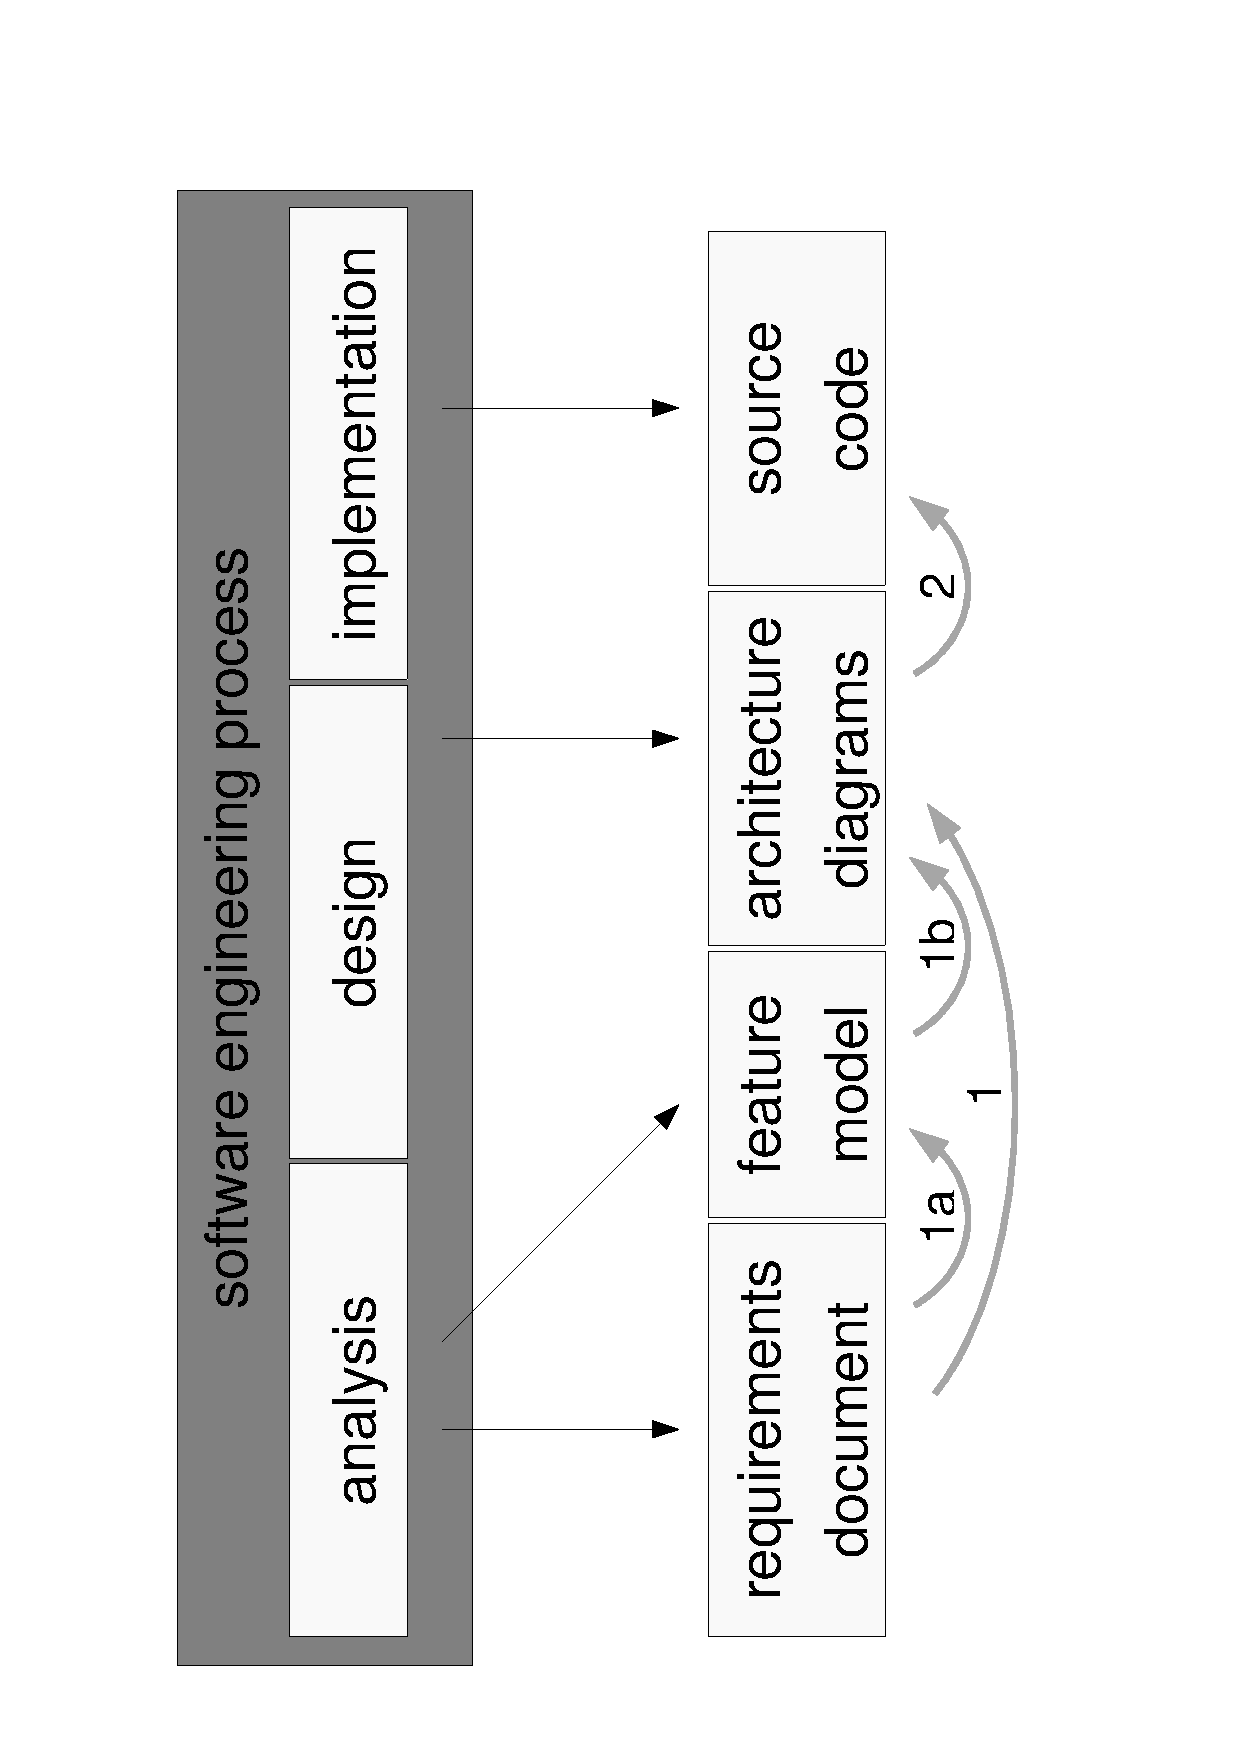
\includegraphics[scale=0.3,angle=-90]{graphics/gaps.pdf}
        \caption{Standard Software Engineering Process}
        \label{software_engineering_process_figure}
    \end{center}
\end{figure}

%
% $RCSfile: interpretation.tex,v $
%
% Copyright (c) 2002-2007. Christian Heller. All rights reserved.
%
% Permission is granted to copy, distribute and/or modify this document
% under the terms of the GNU Free Documentation License, Version 1.1 or
% any later version published by the Free Software Foundation; with no
% Invariant Sections, with no Front-Cover Texts and with no Back-Cover
% Texts. A copy of the license is included in the section entitled
% "GNU Free Documentation License".
%
% http://www.cybop.net
% - Cybernetics Oriented Programming -
%
% Version: $Revision: 1.1 $ $Date: 2007-07-17 20:02:36 $ $Author: christian $
% Authors: Christian Heller <christian.heller@tuxtax.de>
%

\subsection{Interpretation}
\label{inerpretation_heading}
\index{Interpretation}

CYBOP
CYBOL
CYBOI

\begin{figure}[ht]
    \begin{center}
        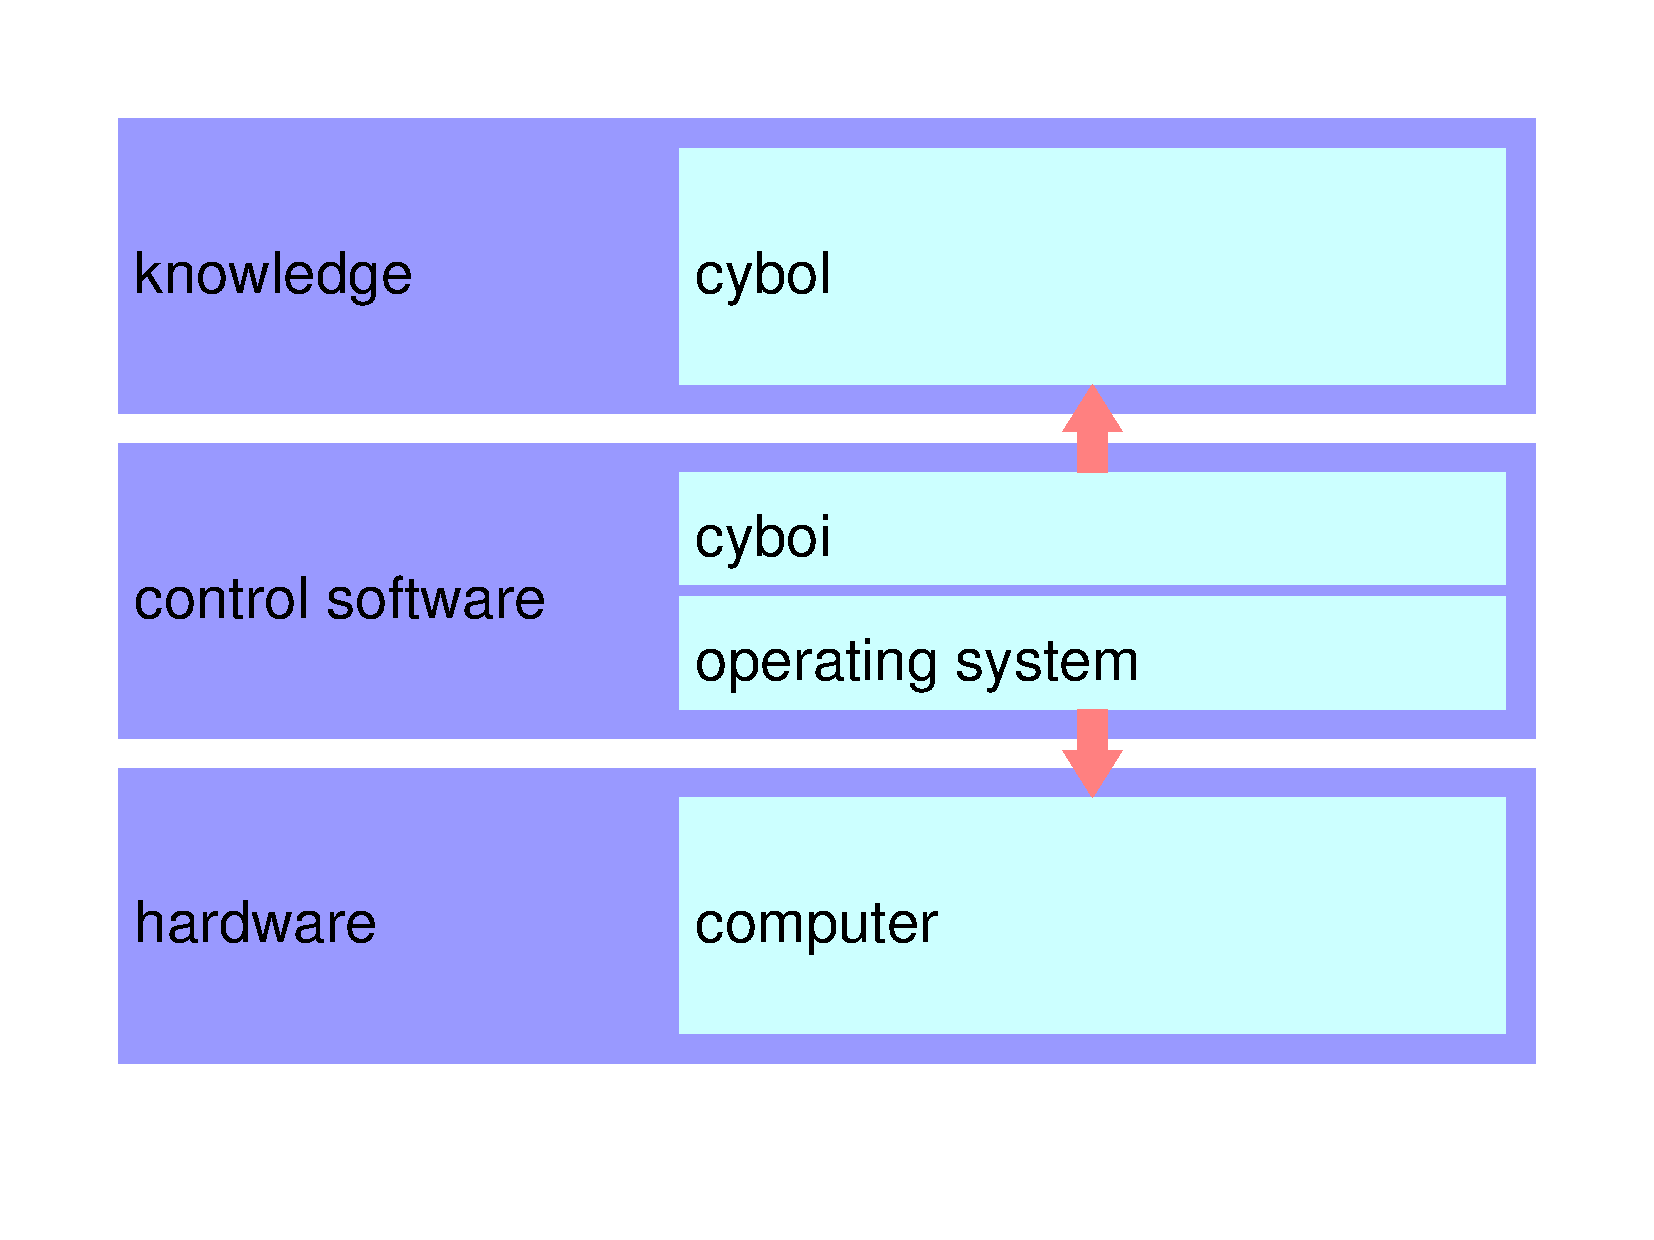
\includegraphics[scale=0.3,angle=-90]{graphics/connection.pdf}
        \caption{CYBOL Interpretation}
        \label{cybol_interpretation_figure}
    \end{center}
\end{figure}


%
% $RCSfile: extensible_markup_language.tex,v $
%
% Copyright (c) 2002-2007. Christian Heller. All rights reserved.
%
% Permission is granted to copy, distribute and/or modify this document
% under the terms of the GNU Free Documentation License, Version 1.1 or
% any later version published by the Free Software Foundation; with no
% Invariant Sections, with no Front-Cover Texts and with no Back-Cover
% Texts. A copy of the license is included in the section entitled
% "GNU Free Documentation License".
%
% http://www.cybop.net
% - Cybernetics Oriented Programming -
%
% Version: $Revision: 1.1 $ $Date: 2007-07-17 20:02:36 $ $Author: christian $
% Authors: Christian Heller <christian.heller@tuxtax.de>
%

\section{Extensible Markup Language}
\label{extensible_markup_language_heading}
\index{Extensible Markup Language}

The \emph{Extensible Markup Language} (XML) is ...


    %
% $RCSfile: basic_patterns.tex,v $
%
% Copyright (c) 2001-2004. Christian Heller. All rights reserved.
%
% No copying, altering, distribution or any other actions concerning this
% document, except after explicit permission by the author!
% At some later point in time, this document is planned to be put under
% the GNU FDL license. For now, _everything_ is _restricted_ by the author.
%
% http://www.cybop.net
% - Cybernetics Oriented Programming -
%
% http://www.resmedicinae.org
% - Information in Medicine -
%
% @author Christian Heller <christian.heller@tuxtax.de>
%

\section{Basic Patterns}
\label{basic_patterns_heading}

%
% $RCSfile: data_mapper.tex,v $
%
% Copyright (c) 2004. Christian Heller. All rights reserved.
%
% No copying, altering, distribution or any other actions concerning this
% document, except after explicit permission by the author!
% At some later point in time, this document is planned to be put under
% the GNU FDL license. For now, _everything_ is _restricted_ by the author.
%
% http://www.cybop.net
% - Cybernetics Oriented Programming -
%
% http://www.resmedicinae.org
% - Information in Medicine -
%
% @author Christian Heller <christian.heller@tuxtax.de>
%

\paragraph{Data Mapper}
\label{data_mapper_heading}

Besides the \emph{Domain Logic}, standard three-tier architectures contain a
\emph{Data Source} layer which may for example represent a database. Both layers
need to exchange data. Modern systems use OOP methods to implement the domain
model. Database models, on the other hand, are often implemented as
\emph{Entity Relationship Model} (ERM).

In order to avoid close coupling and a mix-up of both layers, the introduction
of an additional \emph{Data Mapper} layer \cite{fowler2002} in between the two
others may be justified (figure \ref{datamapper_figure}). The most important
idea of this pattern is to abolish the interdependencies of domain- and
persistence model (database).

\begin{figure}[ht]
    \begin{center}
        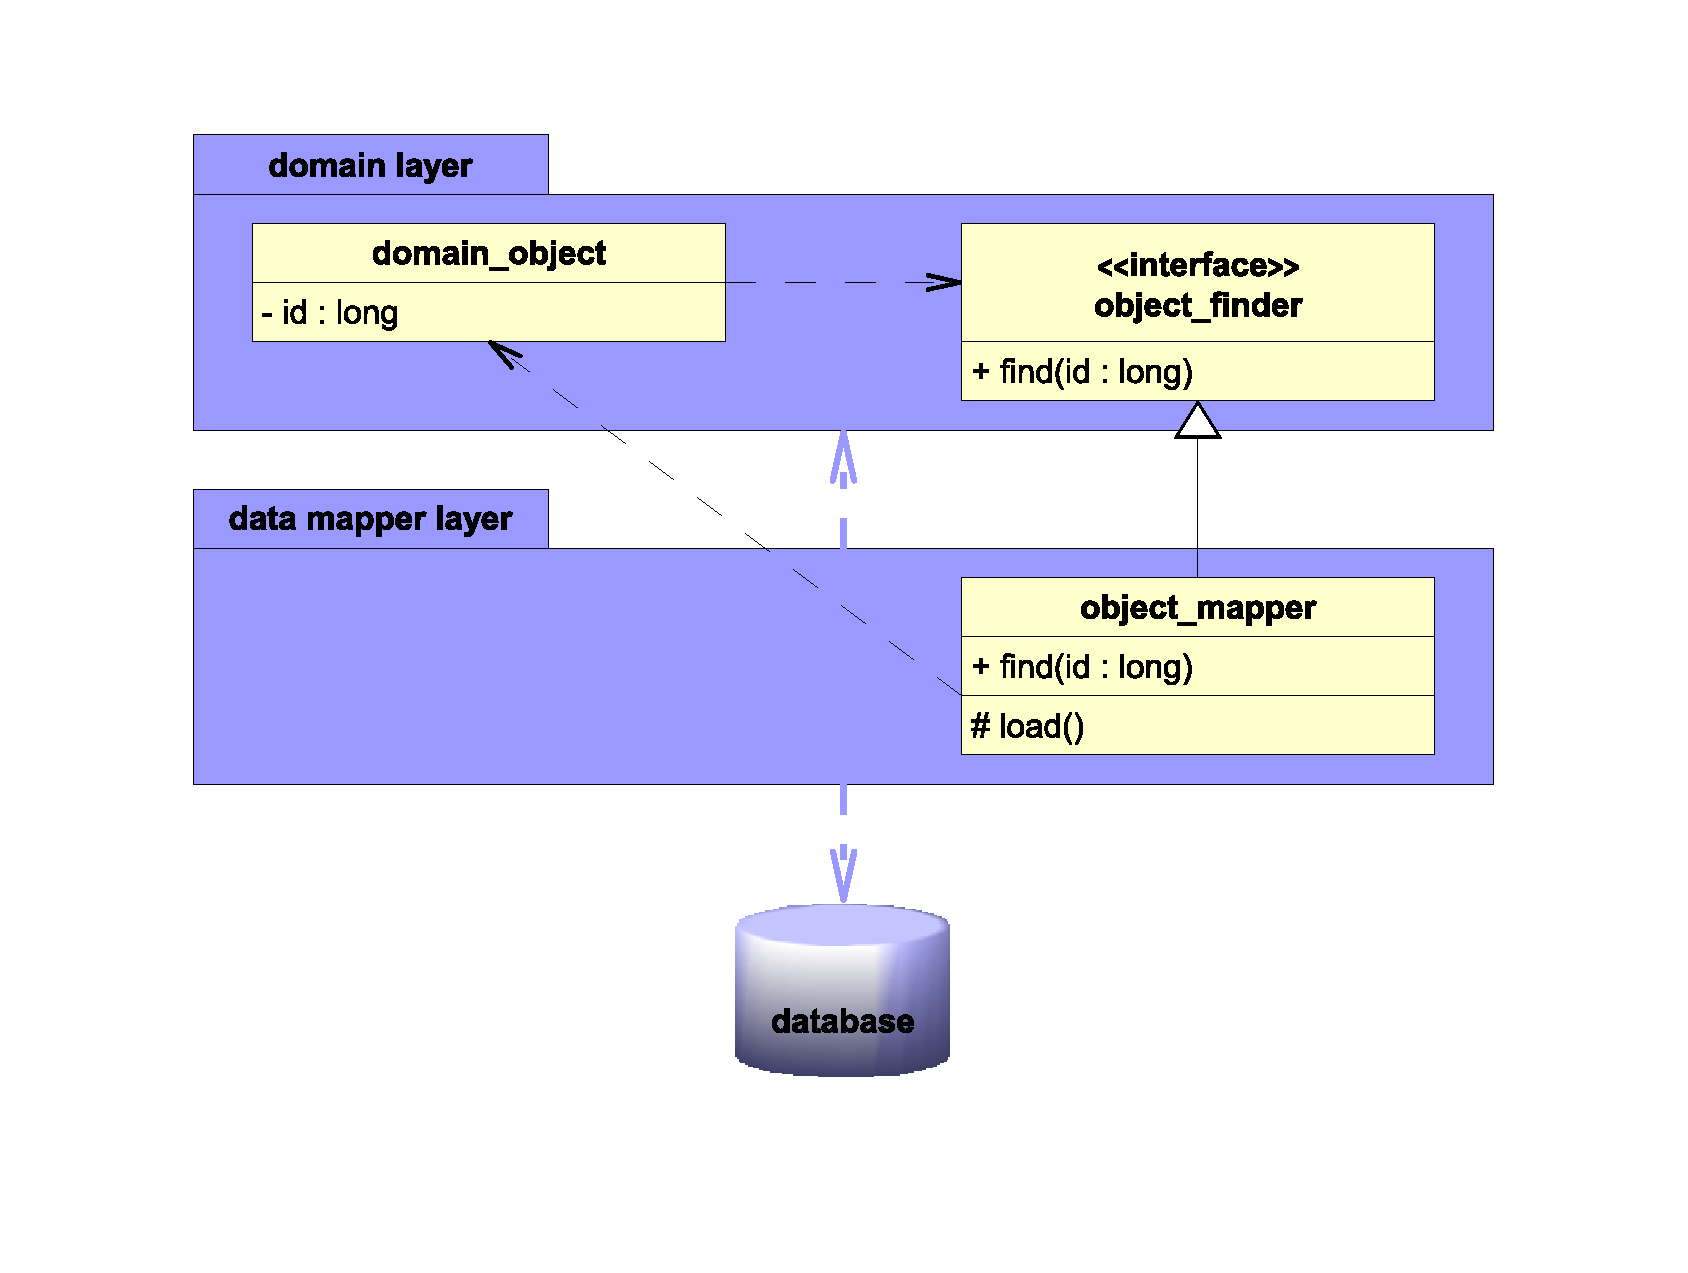
\includegraphics[scale=0.3]{vector/datamapper.eps}
        \caption{Data Mapper Pattern}
        \label{datamapper_figure}
    \end{center}
\end{figure}

The dashed arrows in figure \ref{datamapper_figure} indicate dependencies. The
data mapper layer knows the domain model- as well as the data source layer, via
\emph{unidirectional} relations. Its task is to \emph{translate} between the two,
in both directions. Domain model and data source know nothing from each other.

Each domain model class knows its appropriate interface (\emph{object\_finder})
but does not know the implementation of the same. That is, persistence- and
data retrieval mechanisms are hidden in front of the domain model. The
implementation (\emph{object\_mapper}) is part of the mapping package and also
implements all finder methods. It maps data of the received result sets to the
special attributes of the domain model objects.

The \emph{Mediator} pattern \cite{gamma1995} is similar to the \emph{Mapper}, in
that it is used to decouple different parts of a system. Fowler \cite{fowler2002}
writes: \textit{\ldots the objects that use a mediator are aware of it, even if
they aren't aware of each other; the objects that a mapper separates aren't even
aware of the mapper.}

Although the \emph{Data Mapper} pattern is very helpful at implementing OO
systems, two things are to be criticised:

Firstly, since the \emph{object\_finder} relies on functionality specific to the
retrieval of persistent data, it does actually belong into the data mapper layer
what, if done, would create bidirectional dependencies between the domain model-
and data mapper layer. But also with the \emph{object\_finder} remaining in the
domain model layer, dependencies are not purely unidirectional. It is true that
from an OO view, they are. Internally, however, a super class or interface
relates to its inheriting classes, so that it can call their methods to satisfy
the polymorphic behaviour.

Secondly, the layers do not truely build on each other. Taken a standard
architecture consisting of the following five -- instead of only three -- layers:

\begin{enumerate}
    \item Presentation
    \item Application Process
    \item Domain Model
    \item Data Mapper
    \item Data Source
\end{enumerate}

\ldots the application process does not only access the domain model layer, it
also has to manage (create and destroy) the objects of the data mapper layer.
In other words, it surpasses (disregards) the domain model layer when accessing
the data mapper layer directly.

%
% $RCSfile: data_transfer_object.tex,v $
%
% Copyright (C) 2002-2008. Christian Heller.
%
% Permission is granted to copy, distribute and/or modify this document
% under the terms of the GNU Free Documentation License, Version 1.1 or
% any later version published by the Free Software Foundation; with no
% Invariant Sections, with no Front-Cover Texts and with no Back-Cover
% Texts. A copy of the license is included in the section entitled
% "GNU Free Documentation License".
%
% http://www.cybop.net
% - Cybernetics Oriented Programming -
%
% http://www.resmedicinae.org
% - Information in Medicine -
%
% Version: $Revision: 1.1 $ $Date: 2008-08-19 20:41:06 $ $Author: christian $
% Authors: Christian Heller <christian.heller@tuxtax.de>
%

\subsubsection{Data Transfer Object}
\label{data_transfer_object_heading}
\index{Data Transfer Object Pattern}
\index{DTO}
\index{Assembler Object}
\index{Flat Data Structure}
\index{Translator Architecture}

\begin{figure}[ht]
    \begin{center}
       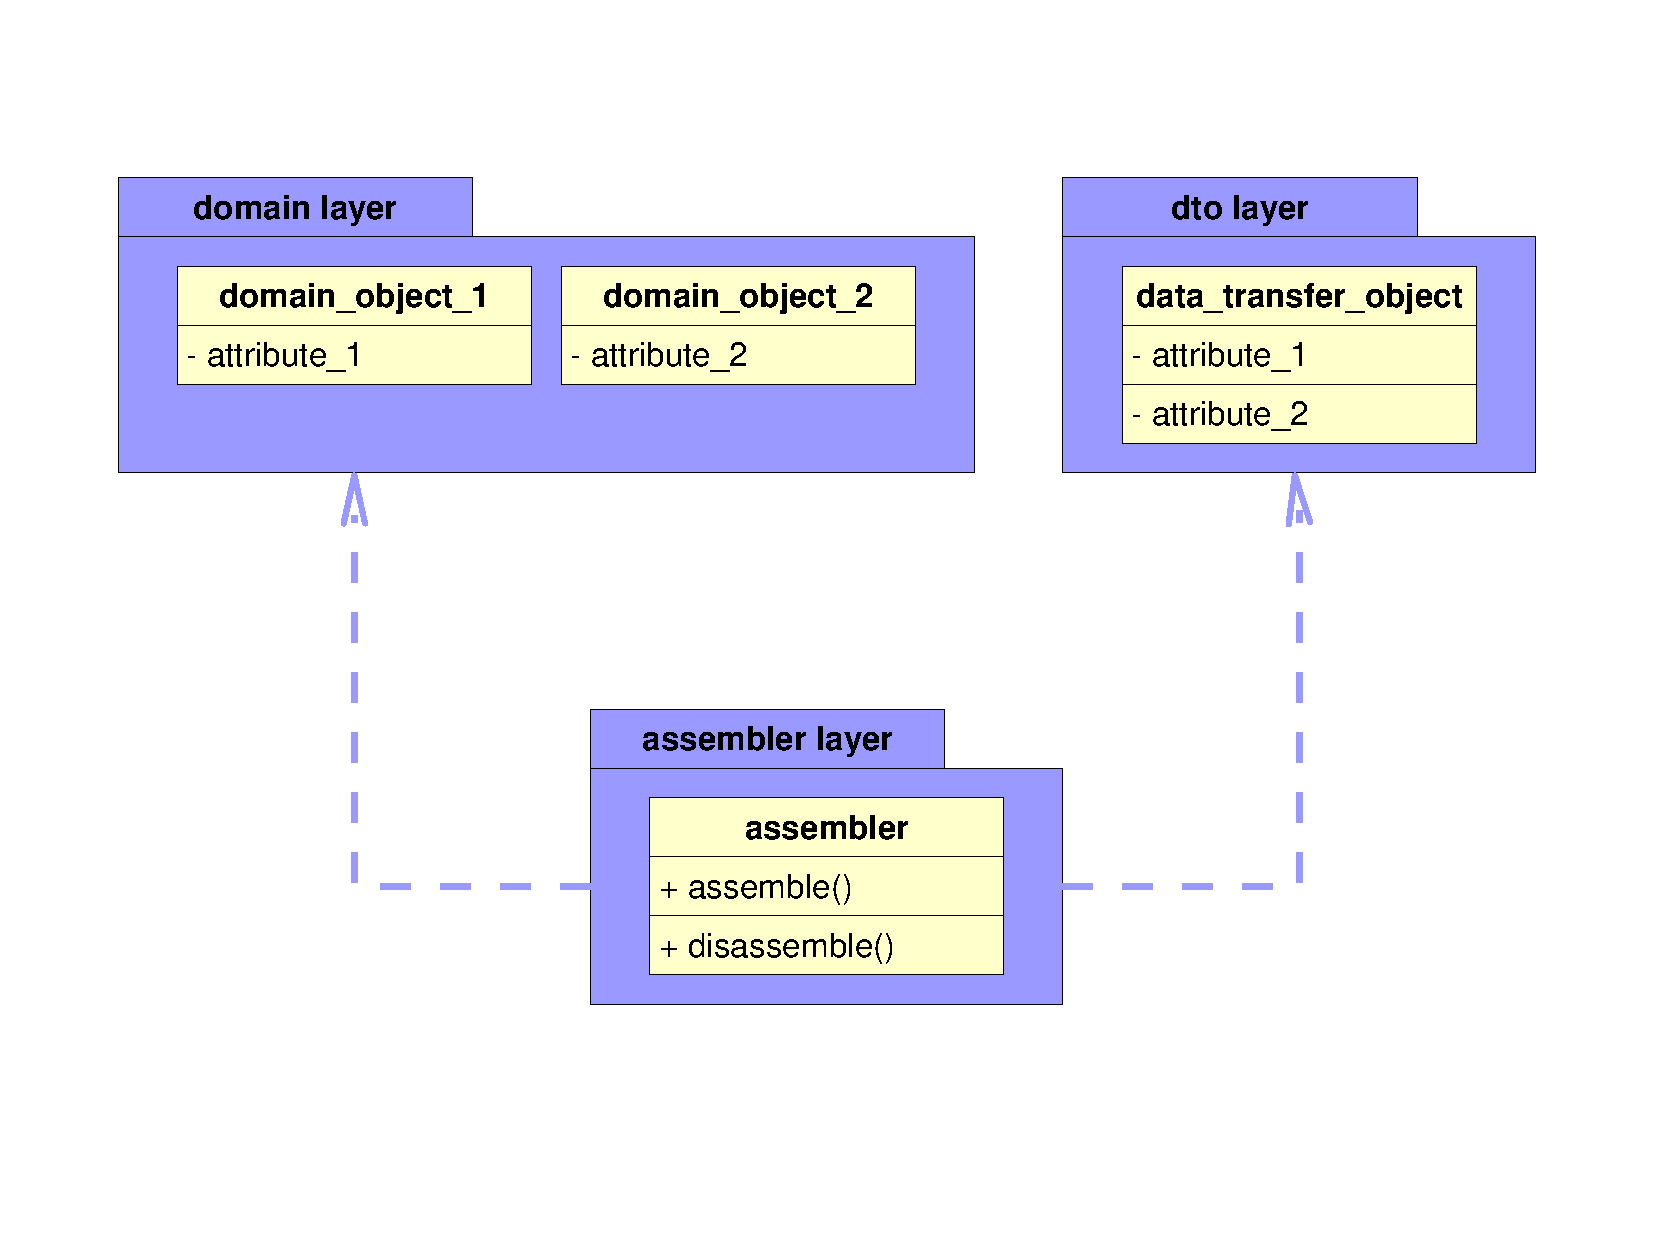
\includegraphics[scale=0.3,angle=-90]{graphic/dto.pdf}
       \caption{Data Transfer Object Pattern}
       \label{dto_figure}
    \end{center}
\end{figure}

It is a well-known fact that many small requests between two processes, and
even more between two hosts in a network need a lot of time. A local machine
with two processes has to permanently change the \emph{Program Context}; a
network has a lot of \emph{Transfers}. For each request, there is a necessity
of at least \emph{two} transfers -- the \emph{Question} of the client and the
\emph{Answer} of the server. Transfer methods are often expected to deliver
common data such as a Person's address, that is surname, first name, street,
zip-code, town and so on. These information is best retrieved by only
\emph{one} transfer call. That way, the client has to wait only once for a
server response and the server does not get too many single tasks. All address
data (in this example) would best be packaged together and sent back to the
client.

A scenario of that kind is exactly what the \emph{Data Transfer Object} pattern
\cite{fowler2002} proposes a solution for: A central \emph{Assembler} object
takes all common data of the server's domain model objects and assembles them
together into a special \emph{Data Transfer Object} (DTO), which is a flat data
structure (figure \ref{dto_figure}). The server will then send this DTO over
network to the client. On the client's side, a similar assembler takes the DTO,
finds out all received data and maps (disassembles) them to the client's domain
model. In that manner, a DTO is able to drastically improve the communication
performance.

Both, \emph{Data Mapper-} and DTO pattern translate one model into another. Due
to this similarity, chapter \ref{state_and_logic_heading} will try to merge
them into a common \emph{Translator} architecture.

%
% $RCSfile: model_view_controller.tex,v $
%
% Copyright (C) 2002-2008. Christian Heller.
%
% Permission is granted to copy, distribute and/or modify this document
% under the terms of the GNU Free Documentation License, Version 1.1 or
% any later version published by the Free Software Foundation; with no
% Invariant Sections, with no Front-Cover Texts and with no Back-Cover
% Texts. A copy of the license is included in the section entitled
% "GNU Free Documentation License".
%
% http://www.cybop.net
% - Cybernetics Oriented Programming -
%
% http://www.resmedicinae.org
% - Information in Medicine -
%
% Version: $Revision: 1.1 $ $Date: 2008-08-19 20:41:07 $ $Author: christian $
% Authors: Christian Heller <christian.heller@tuxtax.de>
%

\subsubsection{Model View Controller}
\label{model_view_controller_heading}
\index{Model View Controller Pattern}
\index{MVC}
\index{Graphical User Interface}
\index{GUI}
\index{Observer Pattern}
\index{Strategy Pattern}
\index{Wrapper Pattern}
\index{Composite Pattern}
\index{Java Foundation Classes}
\index{JFC}
\index{Microsoft Foundation Classes}
\index{MFC}
\index{Document View MVC Variant}
\index{Translator Architecture}

After having had a closer look at design patterns for persistence
(\emph{Data Mapper}) and communication (\emph{Data Transfer Object}), this
section considers the presentation layer of an application (figure
\ref{logical_figure}), which is often realised in form of a
\emph{Graphical User Interface} (GUI). Nowadays, the well-known
\emph{Model View Controller} (MVC) pattern \cite{buschmann, fowler2002} is used
by a majority of standard business applications. Its principle is to have the
\emph{Model} holding domain data, the \emph{View} accessing and displaying
these data and the \emph{Controller} providing the workflow of the application
by handling any action events happening on the view (figure \ref{mvc_figure}).
This separation eases the creation of applications with many synchronous views
on the same data. Internally, the MVC may consist of design patterns like:

\begin{figure}[ht]
    \begin{center}
        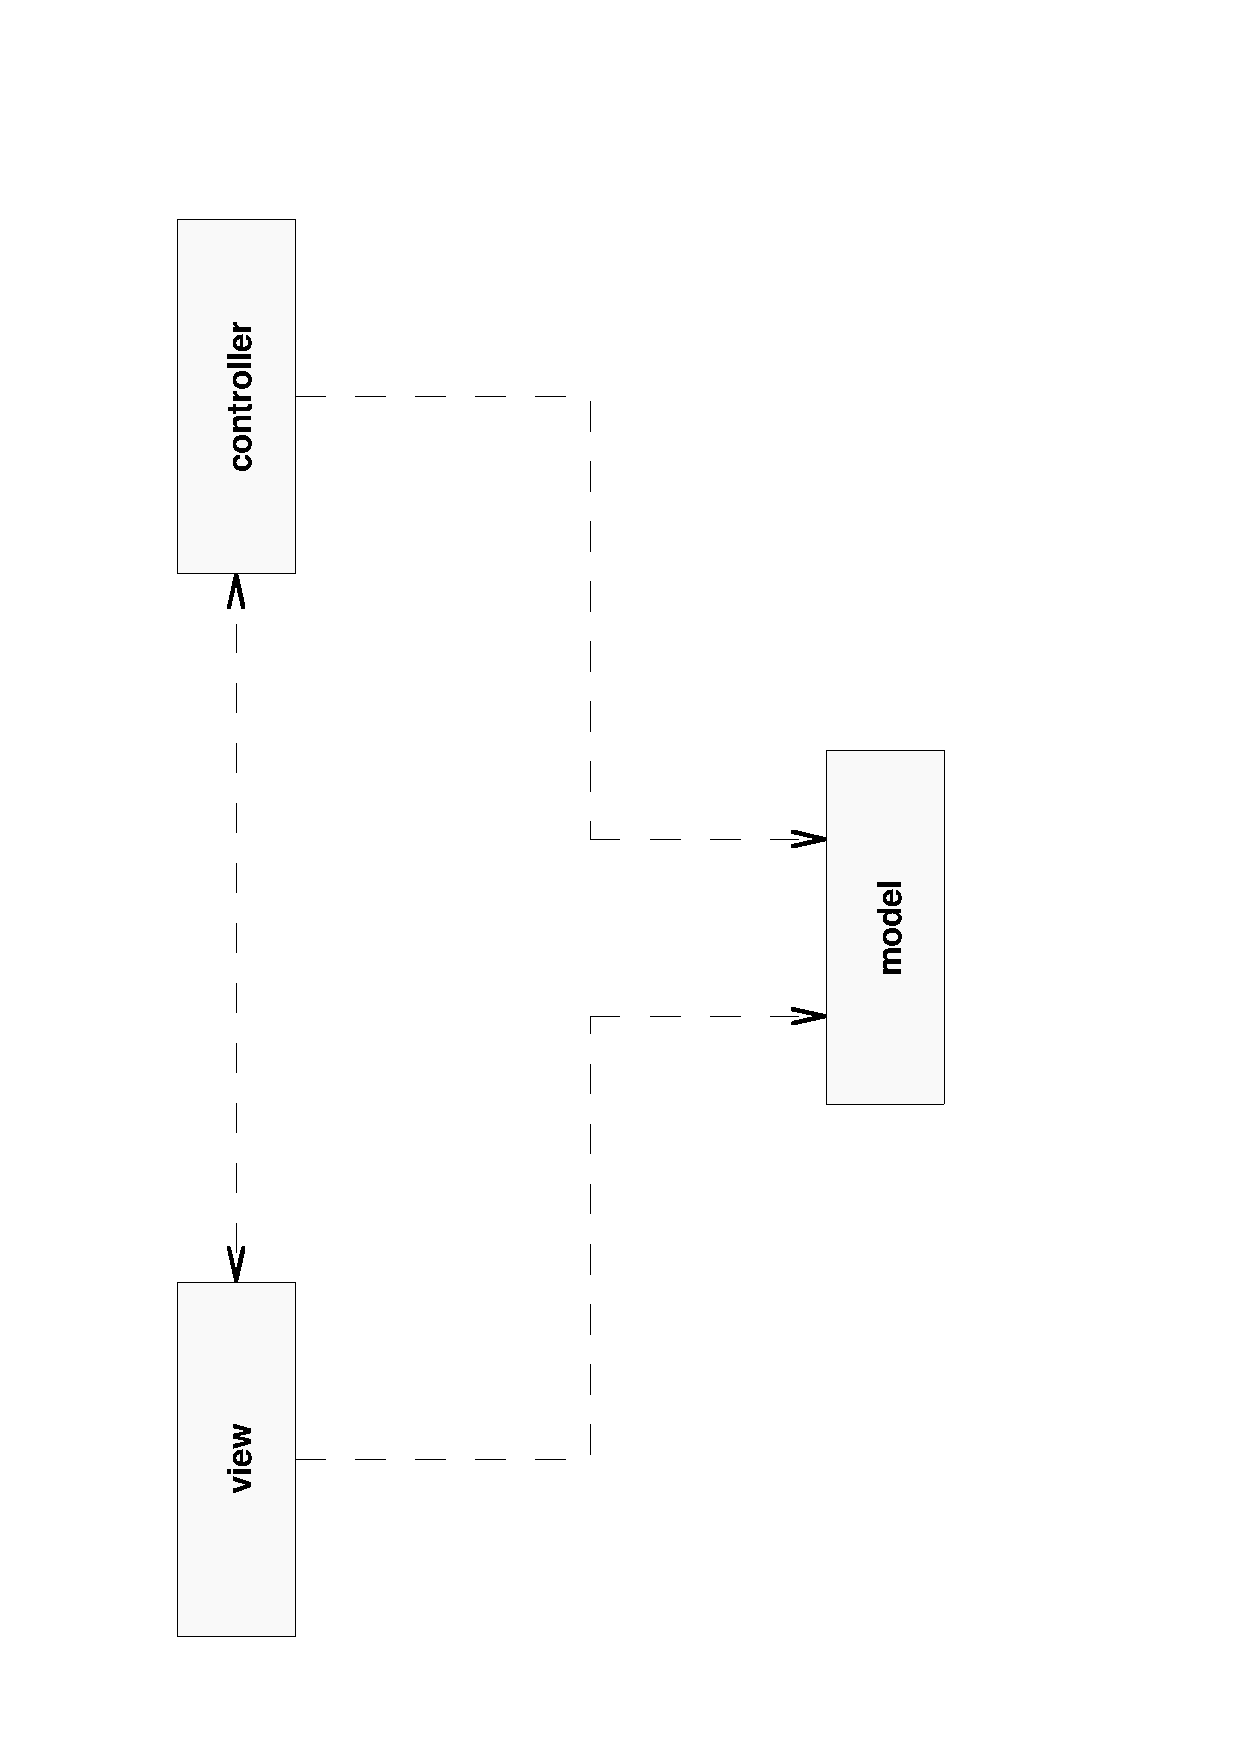
\includegraphics[scale=0.3,angle=-90]{graphic/mvc.pdf}
        \caption{Model View Controller Pattern}
        \label{mvc_figure}
    \end{center}
\end{figure}

\begin{itemize}
    \item[-] \emph{Observer} (section \ref{observer_heading}) which notifies
        the views about data model changes
    \item[-] \emph{Strategy} \cite{gamma1995} which encapsulates exchangeable
        functionality of the controller
    \item[-] \emph{Wrapper} (section \ref{wrapper_heading}) which delegates
        controller functionality to the \emph{Strategy}
    \item[-] \emph{Composite} (section \ref{composite_heading}) which equips
        graphical views with a hierarchical structure
\end{itemize}

Some MVC implementations like parts of the \emph{Java Foundation Classes} (JFC)
use a simplified version not separating controllers from their views. The
\emph{Microsoft Foundation Classes} (MFC) C++ library calls its implementation
\emph{Document-View}.

Besides the above-mentioned patterns \emph{Data Mapper} and DTO, MVC is the
third one getting merged into a common \emph{Translator} architecture, in
chapter \ref{state_and_logic_heading}.



    %
% $RCSfile: hierarchy_and_ontology.tex,v $
%
% Copyright (c) 2001-2004. Christian Heller. All rights reserved.
%
% No copying, altering, distribution or any other actions concerning this
% document, except after explicit permission by the author!
% At some later point in time, this document is planned to be put under
% the GNU FDL license. For now, _everything_ is _restricted_ by the author.
%
% http://www.cybop.net
% - Cybernetics Oriented Programming -
%
% http://www.resmedicinae.org
% - Information in Medicine -
%
% @author Christian Heller <christian.heller@tuxtax.de>
%

\section{Hierarchy and Ontology}
\label{hierarchy_and_ontology_heading}

Section \ref{basic_patterns_heading} explained three design patterns that are
widely used in software architectures. It has shown similarities between them
and raised the question if they could possibly be merged into just one pattern,
called \emph{Translator}, what will be described in section
\ref{logical_architecture_heading}.
Yet before, this section will demonstrate how the principle of \emph{Hierarchy}
may be applied to obtain an \emph{Ontology}.

%
% $RCSfile: association_elimination.tex,v $
%
% Copyright (C) 2002-2008. Christian Heller.
%
% Permission is granted to copy, distribute and/or modify this document
% under the terms of the GNU Free Documentation License, Version 1.1 or
% any later version published by the Free Software Foundation; with no
% Invariant Sections, with no Front-Cover Texts and with no Back-Cover
% Texts. A copy of the license is included in the section entitled
% "GNU Free Documentation License".
%
% http://www.cybop.net
% - Cybernetics Oriented Programming -
%
% http://www.resmedicinae.org
% - Information in Medicine -
%
% Version: $Revision: 1.1 $ $Date: 2008-08-19 20:41:05 $ $Author: christian $
% Authors: Christian Heller <christian.heller@tuxtax.de>
%

\subsection{Association Elimination}
\label{association_elimination_heading}
\index{Association Elimination}
\index{Hierarchy as Principle}
\index{Ontology}
\index{Electronic Health Record}
\index{EHR}
\index{Episode Based EHR}
\index{Object Oriented Programming}
\index{OOP}
\index{Super Model}
\index{Sub Model}
\index{Granularity of Items}
\index{Unidirectional Dependency}
\index{Eliminated Sub Associations}
\index{Ontological Level}
\index{Layers of a System}
\index{Top-most Super Category}

To pursue the idea of a purely hierarchical software system, it seems useful to
investigate in which way domain data models can get simplified. This section
therefore demonstrates how the principle of \emph{Hierarchy} may be applied to
obtain an \emph{Ontology} \cite{hellerkunze}.

\begin{figure}[ht]
    \begin{center}
        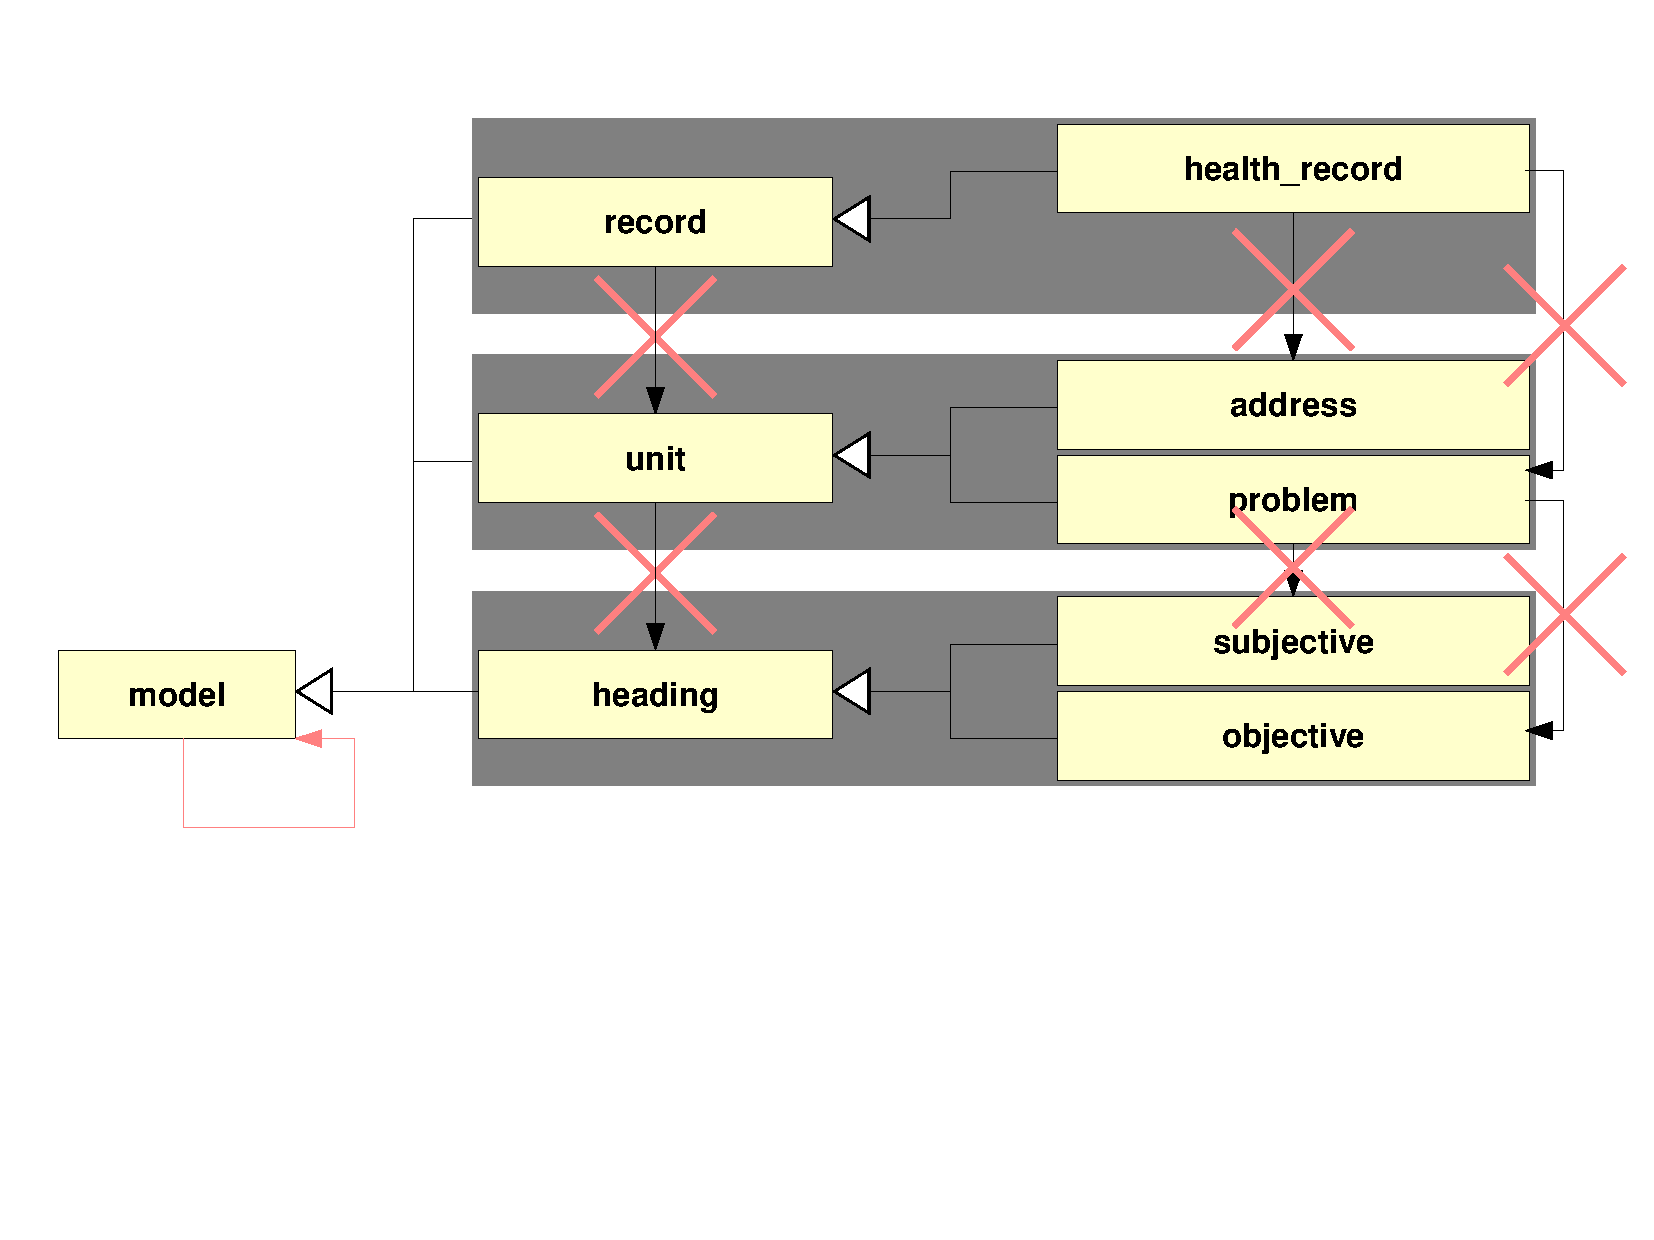
\includegraphics[scale=0.3,angle=-90]{graphic/elimination.pdf}
        \caption{Association Elimination in an EHR}
        \label{elimination_figure}
    \end{center}
\end{figure}

An \emph{Electronic Health Record} (EHR) will serve as example domain model,
whose simplified structure is shown in figure \ref{elimination_figure}. It
consists of numerous parts whereof two may be \emph{Address} and \emph{Problem}.
Following the \emph{Episode-based EHR} recommendation \cite{westerhof},
\emph{Problem} may, besides others, consist of parts of type \emph{Subjective}
and \emph{Objective}. All these associations between part models are needed to
navigate through the overall domain model.

A frequent design decision in classical \emph{Object Oriented Programming}
(OOP) is to sum up common properties of \emph{Sub} models by introducing a
\emph{Super} model (category). It should never be \emph{Properties}, but rather
the \emph{Granularity} of objects leading to the creation of a super category,
as the later section \ref{categorisation_versus_composition_heading} will
recommend. The \emph{OpenEHR} project \cite{openehr} suggests to let the
above-mentioned sub models inherit from the more coarse-grained super
categories \emph{Record}, \emph{Unit} and \emph{Heading}.

Whichever reason -- once the super categories are there, they should be
associated similarly to their sub categories, that is in the same direction,
using solely \emph{unidirectional} dependencies. (The problematic nature of
bidirectional dependencies was elaborated in section \ref{pattern_heading}.)
Afterwards, all associations between sub categories become superfluous as every
sub category can reach its sibling across the super categories' association
(figure \ref{elimination_figure}). In other words:
\emph{Super- eliminate Sub Associations}.

Here a short Java code example for how the \emph{HealthRecord} may retrieve a
reference to \emph{Address}:

\begin{scriptsize}
    \begin{verbatim}
    Address a = (Address) get_element("address");
    \end{verbatim}
\end{scriptsize}

\emph{HealthRecord} inherits the \emph{get\_element} method from its super
category \emph{Record}. \emph{Record} holds differing sub models of category
\emph{Unit} and other instances. The \emph{get\_element} method delivers back
a general \emph{Model} that still needs to be down-casted to the expected sub
category \emph{Address}.

\begin{figure}[ht]
    \begin{center}
        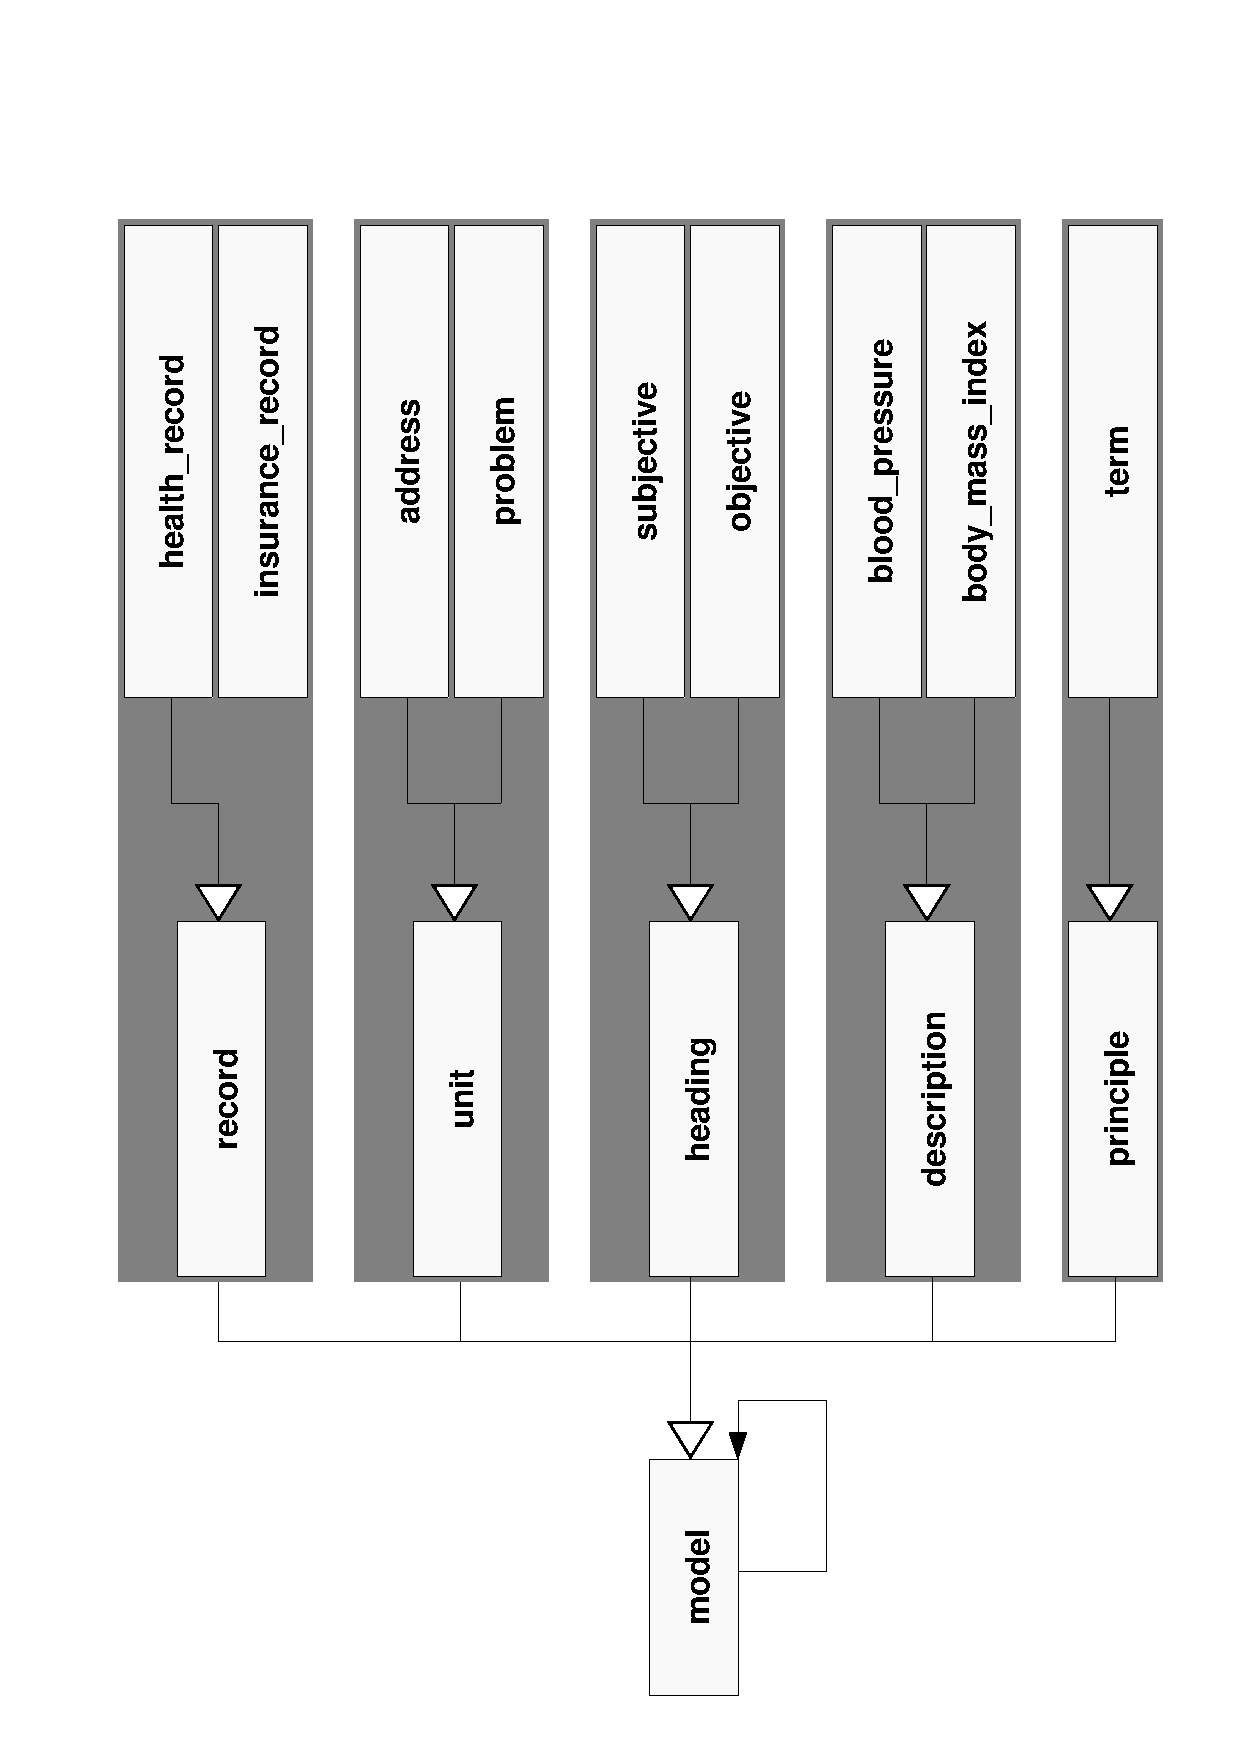
\includegraphics[scale=0.3,angle=-90]{graphic/levels.pdf}
        \caption{Model Container and Ontological Levels}
        \label{levels_figure}
    \end{center}
\end{figure}

The definition of models, their dependencies (defined by associations) and
granularities (defined by inheritance) in a software system results in several
\emph{Layers} of models of common granularity (figure \ref{levels_figure}).
These layers are often called \emph{Ontological Level} as they, together, form
an \emph{Ontology} (sections \ref{ontology_heading},
\ref{knowledge_ontology_heading}).

An ontology of that kind can, of course, be created for every knowledge model.
The financial sector -- like an insurance company, for example -- may use an
\emph{Insurance Record} with comparable structure.

The idea to structure software as a system of \emph{Layers} was also suggested
by the equally named pattern in section \ref{layers_heading}. The difference
between the two is that the \emph{Layers} pattern divides a system only by its
\emph{Functionality}, for example into \emph{User Interface}, \emph{Domain},
\emph{Data Mapper} and \emph{Data Source}. An \emph{Ontology} additionally
groups model items by their \emph{Granularity}. By inheriting from a common
superior category, sub categories indicate that they logically belong to the
same \emph{Layer}.

Continuing the structuring process of introducing more and more common super
categories, for all equally-granular items, the development culminates in one
top-most super category of all other categories in the system, which this paper
calls \emph{Model}. It is as general as the \emph{java.lang.Object} class for
the Java class library \cite{java}, only that it additionally represents a
\emph{Container} that can store models of any category, as explained in
\cite{hellerbohl}. In other words, \emph{Model} provides the meta functionality
of a container behaviour to \emph{all} other categories in a system.

%
% $RCSfile: ontology.tex,v $
%
% Copyright (c) 2001-2004. Christian Heller. All rights reserved.
%
% No copying, altering, distribution or any other actions concerning this
% document, except after explicit permission by the author!
% At some later point in time, this document is planned to be put under
% the GNU FDL license. For now, _everything_ is _restricted_ by the author.
%
% http://www.cybop.net
% - Cybernetics Oriented Programming -
%
% http://www.resmedicinae.org
% - Information in Medicine -
%
% @author Christian Heller <christian.heller@tuxtax.de>
%

\subsection{Ontology}
\label{ontology_heading}

Manifold definitions of the word \emph{Ontology} exist. They come from philosophy,
metaphysics, information technology and others -- too many to list here.
This document uses its own, adapted definition and considers an ontology to be
\emph{a strict hierarchy of abstract items, organized in levels of growing
granularity, that are solely unidirectionally related}. It such represents a
systematic description of complex domain contexts.

\begin{figure}[ht]
    \begin{center}
        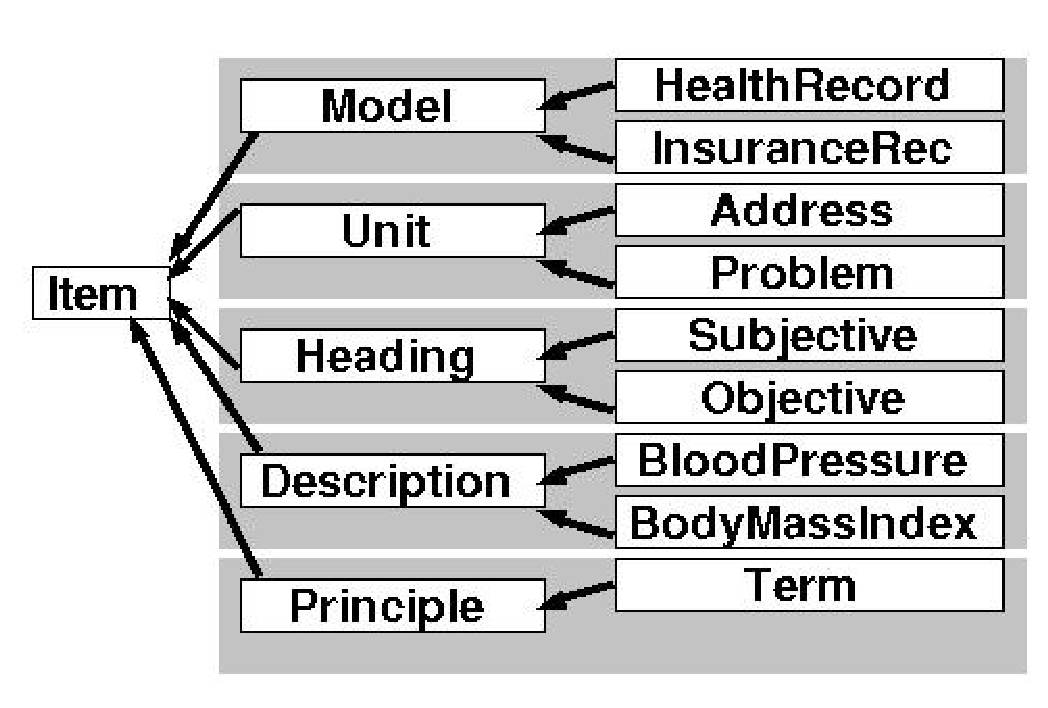
\includegraphics[scale=0.4]{vector/electronic_health_record_ontology.eps}
        \caption{Electronic Health Record Ontology}
        \label{electronic_health_record_ontology_figure}
    \end{center}
\end{figure}

Figure \ref{electronic_health_record_ontology_figure} shows one possible ontology
of an electronic health record, as described in the previous section.




    %
% $RCSfile: logical_architecture.tex,v $
%
% Copyright (c) 2001-2004. Christian Heller. All rights reserved.
%
% No copying, altering, distribution or any other actions concerning this
% document, except after explicit permission by the author!
% At some later point in time, this document is planned to be put under
% the GNU FDL license. For now, _everything_ is _restricted_ by the author.
%
% http://www.cybop.net
% - Cybernetics Oriented Programming -
%
% http://www.resmedicinae.org
% - Information in Medicine -
%
% @author Christian Heller <christian.heller@tuxtax.de>
%

\section{Logical Architecture}
\label{logical_architecture_heading}

This section will sort the design patterns of section \ref{basic_patterns_heading}
into the layered architecture of a standard application. Afterwards, the
hierarchical principles of section \ref{hierarchy_and_ontology_heading} are applied
to simplify and merge the design patterns which will lead to an ontology.

\begin{figure}[ht]
    \begin{center}
        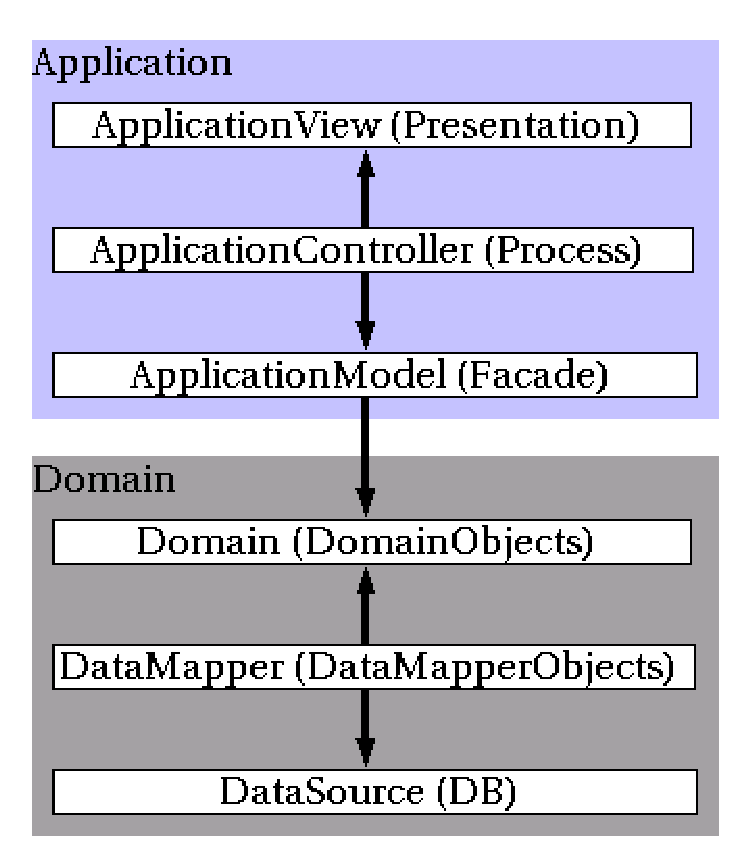
\includegraphics[scale=0.3]{vector/layered_architecture.eps}
        \caption{Layered Architecture}
        \label{layered_architecture_figure}
    \end{center}
\end{figure}

A state-of-the-art software system consists of a layered architecture similar to the
one shown in figure \ref{layered_architecture_figure}. The startable \emph{Controller}
process creates the whole application tree, to which belong the \emph{View} (as
user interface), the \emph{Model} (providing data to the view and as facade to
remote servers) and the \emph{Domain} with its database \emph{Mapper} layer.\\
It is not difficult to figure out where the basic patterns of section \ref{basic_patterns_heading}
fit in here (figure \ref{layered_architecture_with_basic_patterns_figure}):
The \emph{Model View Controller} pattern determines the classes to interact with
a human user via the \emph{View} (sometimes called \emph{Presentation Layer});
the \emph{Data Mapper} pattern provides necessary classes and an \emph{Entity
Relationship Model} (ERM) to connect to a persistence medium such as a database;
the \emph{Data Transfer Object} (DTO) pattern, finally, serves as means of
communication with remote servers.

\begin{figure}[ht]
    \begin{center}
        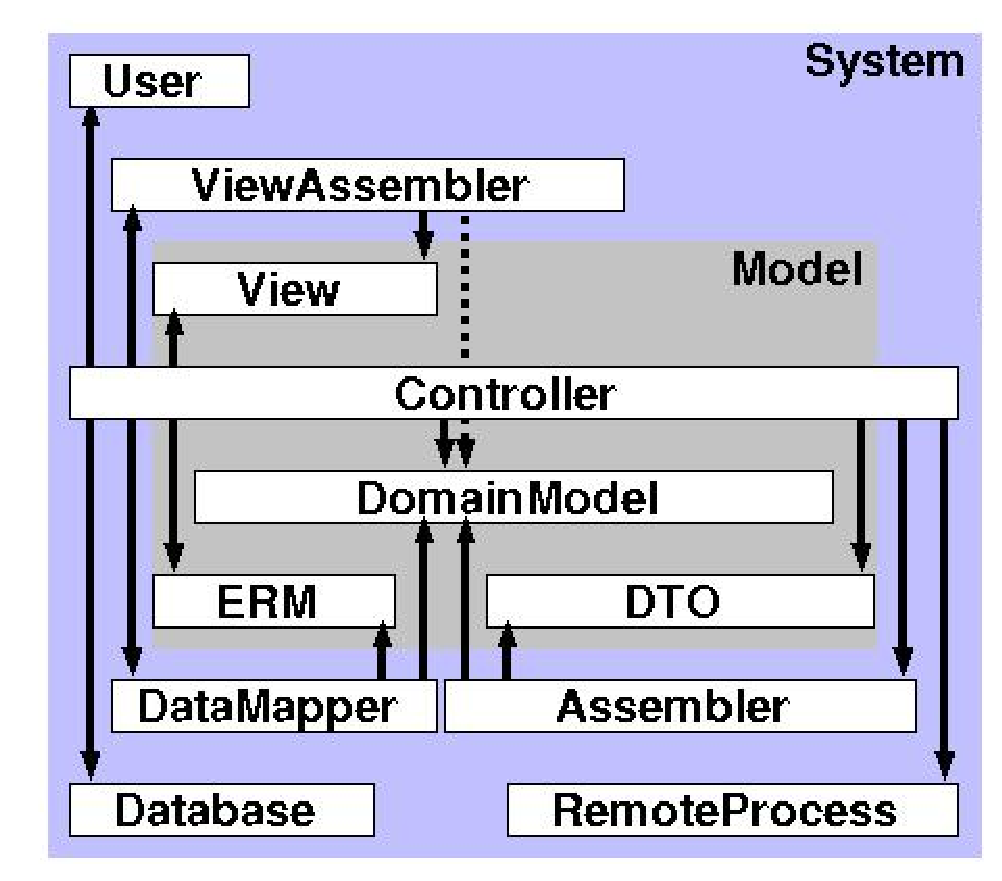
\includegraphics[scale=0.3]{vector/layered_architecture_with_basic_patterns.eps}
        \caption{Layered Architecture with Basic Patterns}
        \label{layered_architecture_with_basic_patterns_figure}
    \end{center}
\end{figure}

For all three kinds of communication, there is a:
\begin{itemize}
    \item[-] System (HumanUser, DataBase, RemoteServer)
    \item[-] Model (View, ERM, DTO)
    \item[-] Translator (ViewAssembler, Mapper, DTOAssembler)
\end{itemize}

Realizing this, it is easy to create ontological layers by adding one common
parent class for systems, models and translators each, which leads to a much
clearer architecture (figure \ref{layered_architecture_with_merged_patterns_figure}).
The common properties of all sub classes are merged into their corresponding super
class.

\begin{figure}[ht]
    \begin{center}
        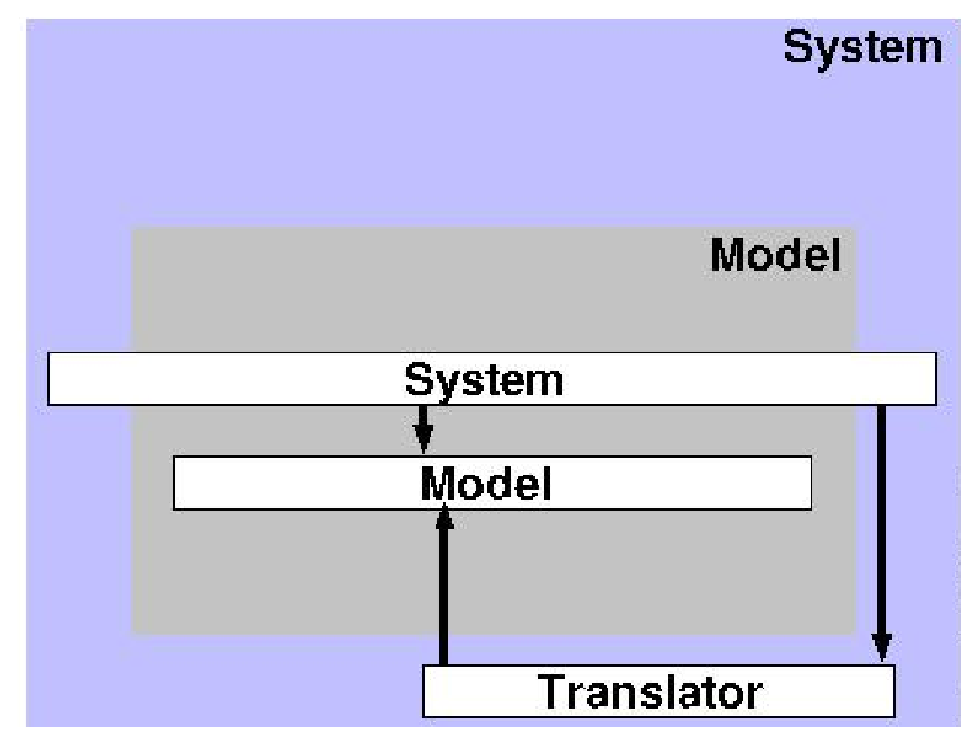
\includegraphics[scale=0.3]{vector/layered_architecture_with_merged_patterns.eps}
        \caption{Layered Architecture with merged Patterns}
        \label{layered_architecture_with_merged_patterns_figure}
    \end{center}
\end{figure}


    %
% $RCSfile: biological_reflections.tex,v $
%
% Copyright (c) 2001-2004. Christian Heller. All rights reserved.
%
% No copying, altering, distribution or any other actions concerning this
% document, except after explicit permission by the author!
% At some later point in time, this document is planned to be put under
% the GNU FDL license. For now, _everything_ is _restricted_ by the author.
%
% http://www.cybop.net
% - Cybernetics Oriented Programming -
%
% http://www.resmedicinae.org
% - Information in Medicine -
%
% @author Christian Heller <christian.heller@tuxtax.de>
%

\section{Biological Reflections}
\label{biological_reflections_heading}

The previous sections have shown how existing patterns for communication can be
merged into one common system architecture. All of these design patterns suggest
their very own communication paradigm which cannot be used anymore in the new,
merged \emph{Translator} architecture. Therefore, a new way for system interaction
needs to be found.

\begin{figure}[ht]
    \begin{center}
        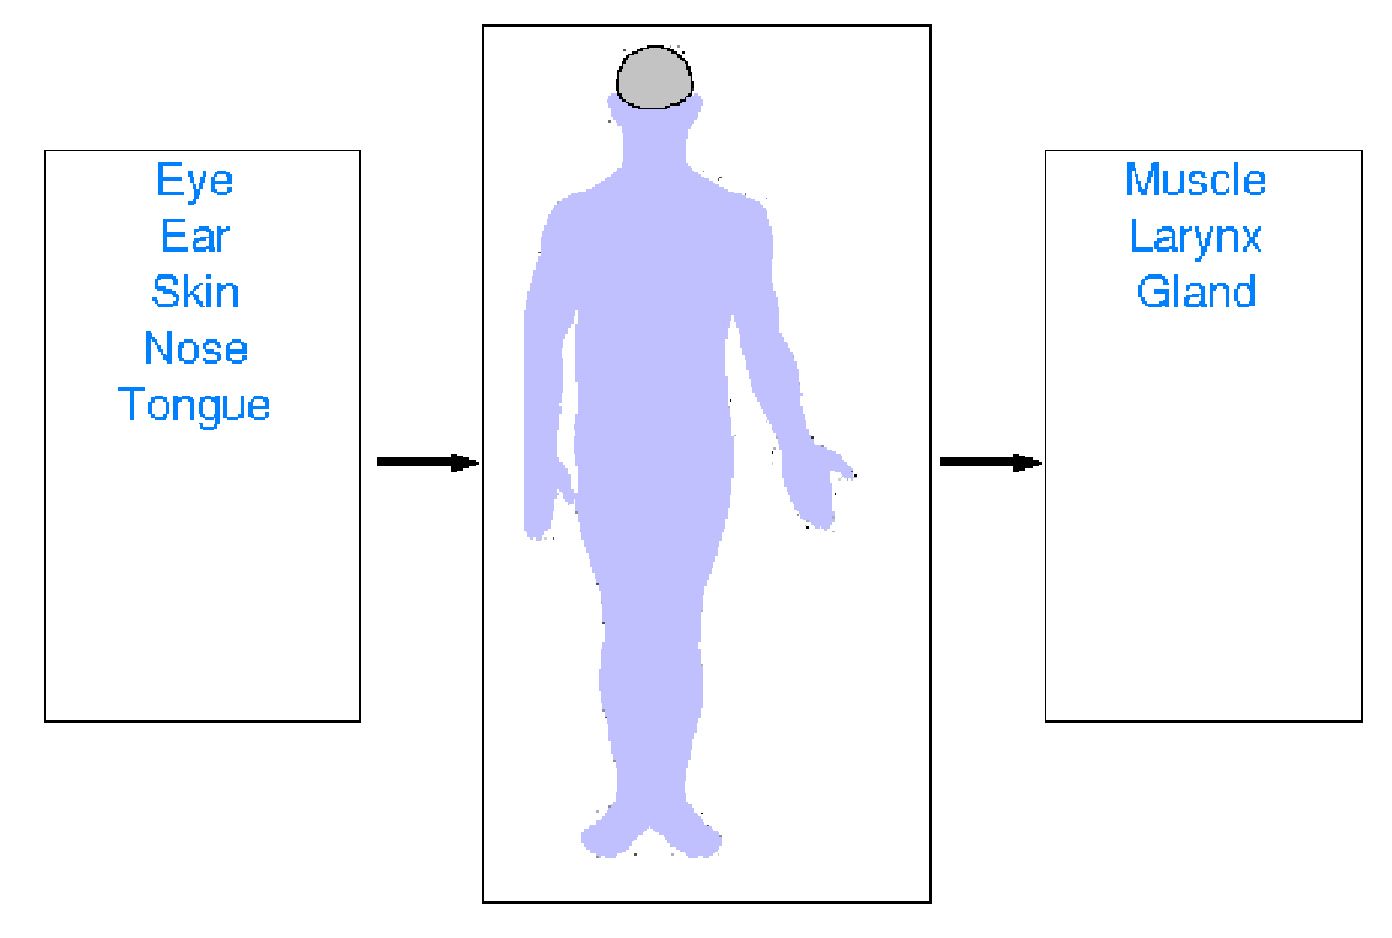
\includegraphics[scale=0.3]{vector/human_being_as_system.eps}
        \caption{Human Being as System of Models (Brain)}
        \label{human_being_as_system_figure}
    \end{center}
\end{figure}

Following the CYBOP approach, nature -- in our case the Human body -- will be
considered next. Humans have organs responsible for information input and output
(figure \ref{human_being_as_system_figure}). In between input and output, the
information is processed by the brain that contains a specific abstract model
of the surrounding real world. The human brain consists of several regions, each
being responsible for a special task, such as the optical region for seeing or the
cerebral cortex for actual information processing which possibly leads to awareness.

\begin{figure}[ht]
    \begin{center}
        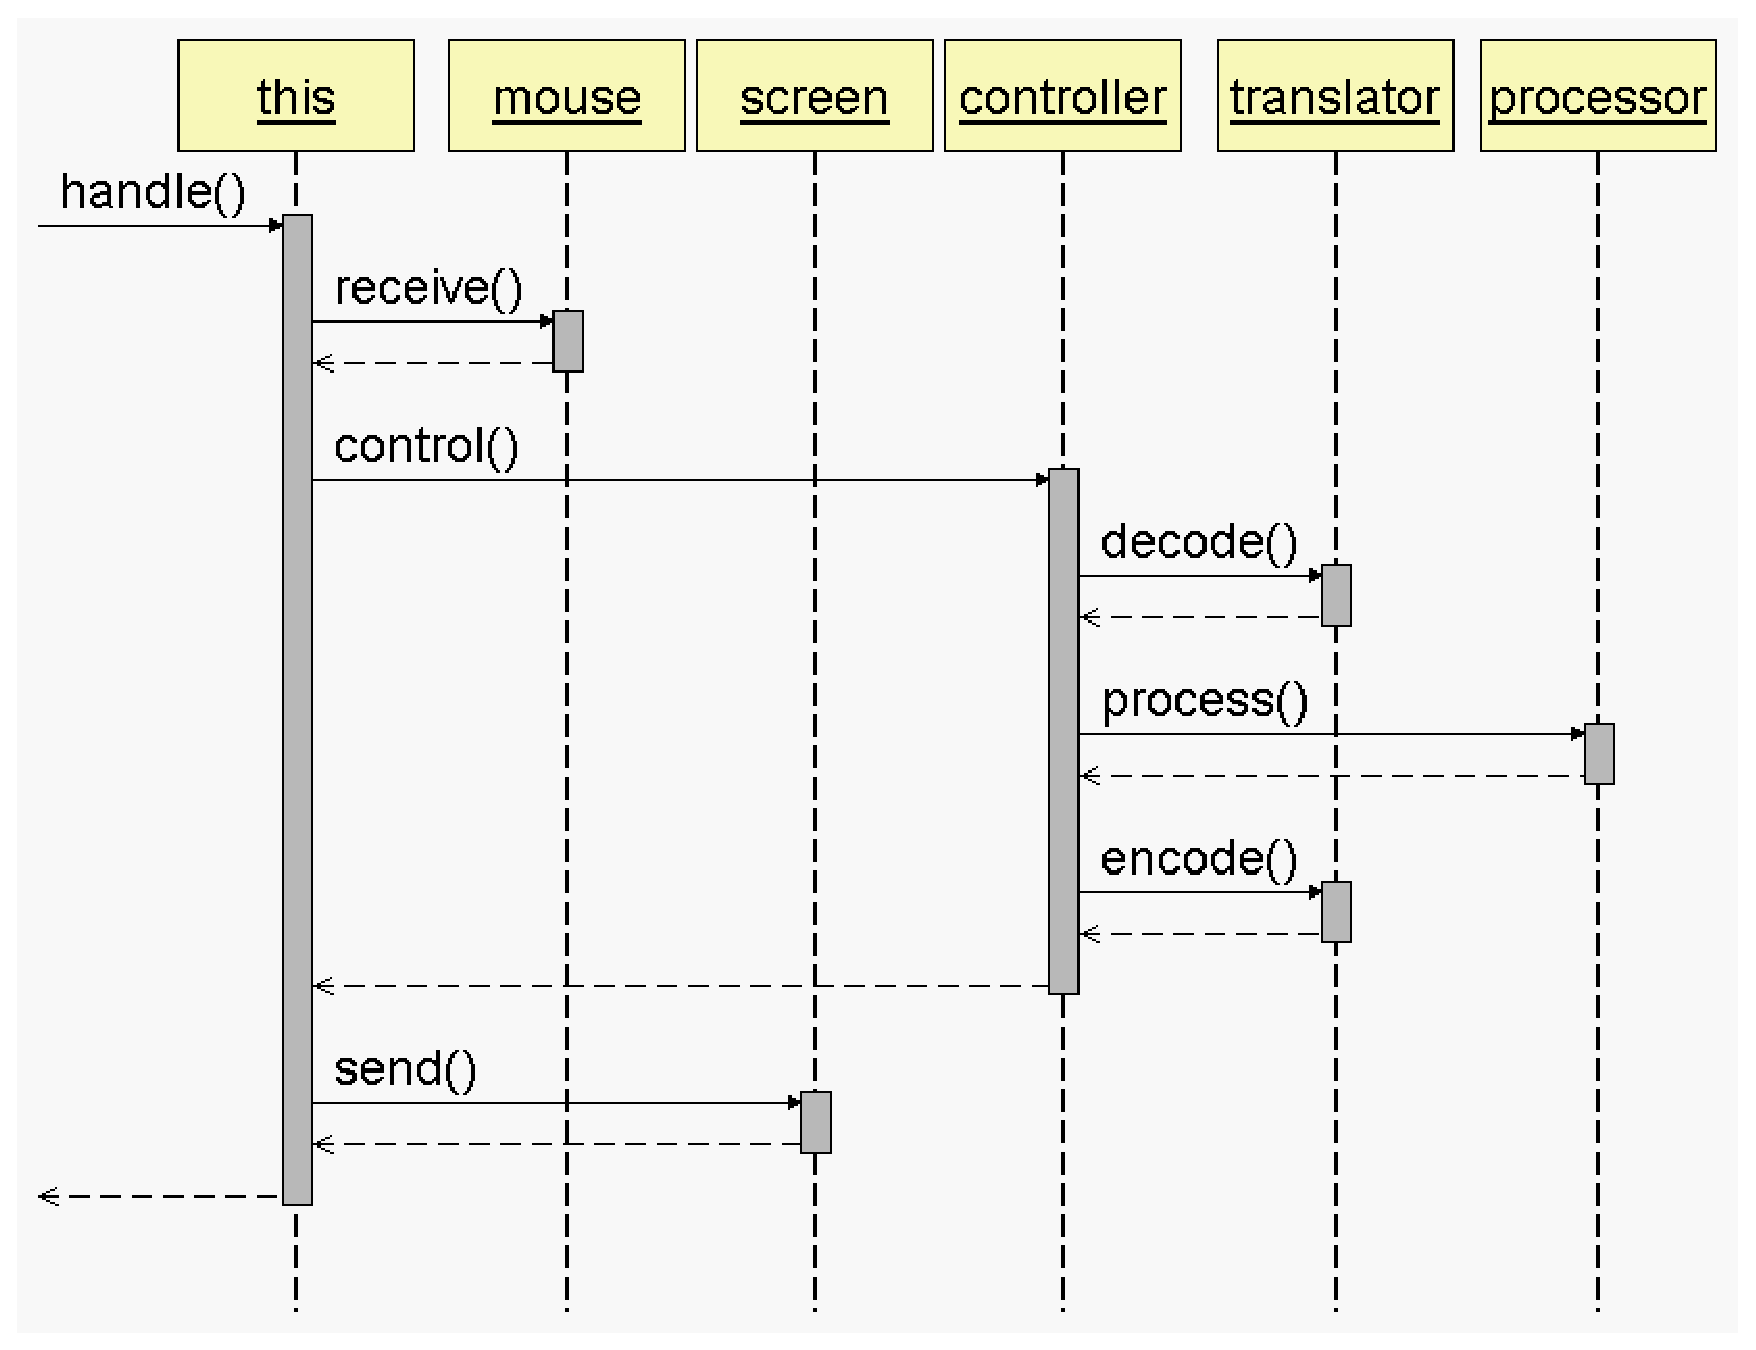
\includegraphics[scale=0.3]{vector/signal_processing.eps}
        \caption{Signal Processing as UML Sequence Diagram}
        \label{signal_processing_figure}
    \end{center}
\end{figure}

The following example demonstrates a typical information (signal) processing
procedure (technical names were used instead of biological ones in figure
\ref{signal_processing_figure}; the terms \emph{Mapper} and \emph{Assembler}
are converted and merged into the term \emph{Translator}):\\
One human \emph{System} wants to send another human \emph{System} a message.
It decides for an acoustical \emph{Signal}, formulates a sentence and talks to
the other human \emph{System} (\emph{handle} method). The other human receives the
\emph{Signal} across its ear organ (\emph{Keyboard}, \emph{Mouse}, \emph{Network}).
The \emph{Signal} is then forwarded to the receiver's brain (\emph{Controller})
where a special \emph{Region} responsible for acoustics (\emph{Translator})
translates (\emph{decode} method) the data (\emph{DataTransferModel}) contained
in the \emph{Signal} and sorts them into the human's abstract model of the
surrounding real world (\emph{DomainModel} or \emph{KnowledgeModel}, respectively).
Processing of the signal happens in the cerebral cortex of the brain (\emph{Processor}).
If the addressed listener wants to send an answer \emph{Signal}, it may do so by
triggering a muscle reaction. For this to happen, the motoric brain region (\emph{Translator})
needs to translate (\emph{encode} method) abstract model data (\emph{DomainModel})
into a special communication model (\emph{UserInterfaceModel}) for the answer signal.
Finally, the answer signal will be sent as muscle action (data display on \emph{Screen}).


    %
% $RCSfile: system_models.tex,v $
%
% Copyright (c) 2001-2004. Christian Heller. All rights reserved.
%
% No copying, altering, distribution or any other actions concerning this
% document, except after explicit permission by the author!
% At some later point in time, this document is planned to be put under
% the GNU FDL license. For now, _everything_ is _restricted_ by the author.
%
% http://www.cybop.net
% - Cybernetics Oriented Programming -
%
% http://www.resmedicinae.org
% - Information in Medicine -
%
% @author Christian Heller <christian.heller@tuxtax.de>
%

\section{System Models}
\label{system_models_heading}

So far, the paper has elaborated on the statics (section \ref{logical_architecture_heading})
as well as the dynamic side (section \ref{biological_reflections_heading}) of the
proposed \emph{Translator} pattern.
This section will finally show the overall results in a number of architecture
diagrams.

%
% $RCSfile: translator_pattern.tex,v $
%
% Copyright (c) 2001-2004. Christian Heller. All rights reserved.
%
% No copying, altering, distribution or any other actions concerning this
% document, except after explicit permission by the author!
% At some later point in time, this document is planned to be put under
% the GNU FDL license. For now, _everything_ is _restricted_ by the author.
%
% http://www.cybop.net
% - Cybernetics Oriented Programming -
%
% http://www.resmedicinae.org
% - Information in Medicine -
%
% @author Christian Heller <christian.heller@tuxtax.de>
%

\subsection{Translator Pattern}
\label{translator_pattern_heading}

As could be seen in section \ref{biological_reflections_heading}, there is always
a \emph{Translator} that is able to map domain model data to communication model
data (\emph{encode} method) and back (\emph{decode} method). Depending on which
communication medium is used, different translators need to be applied (figure
\ref{translator_classes_figure}).

\begin{figure}[ht]
    \begin{center}
        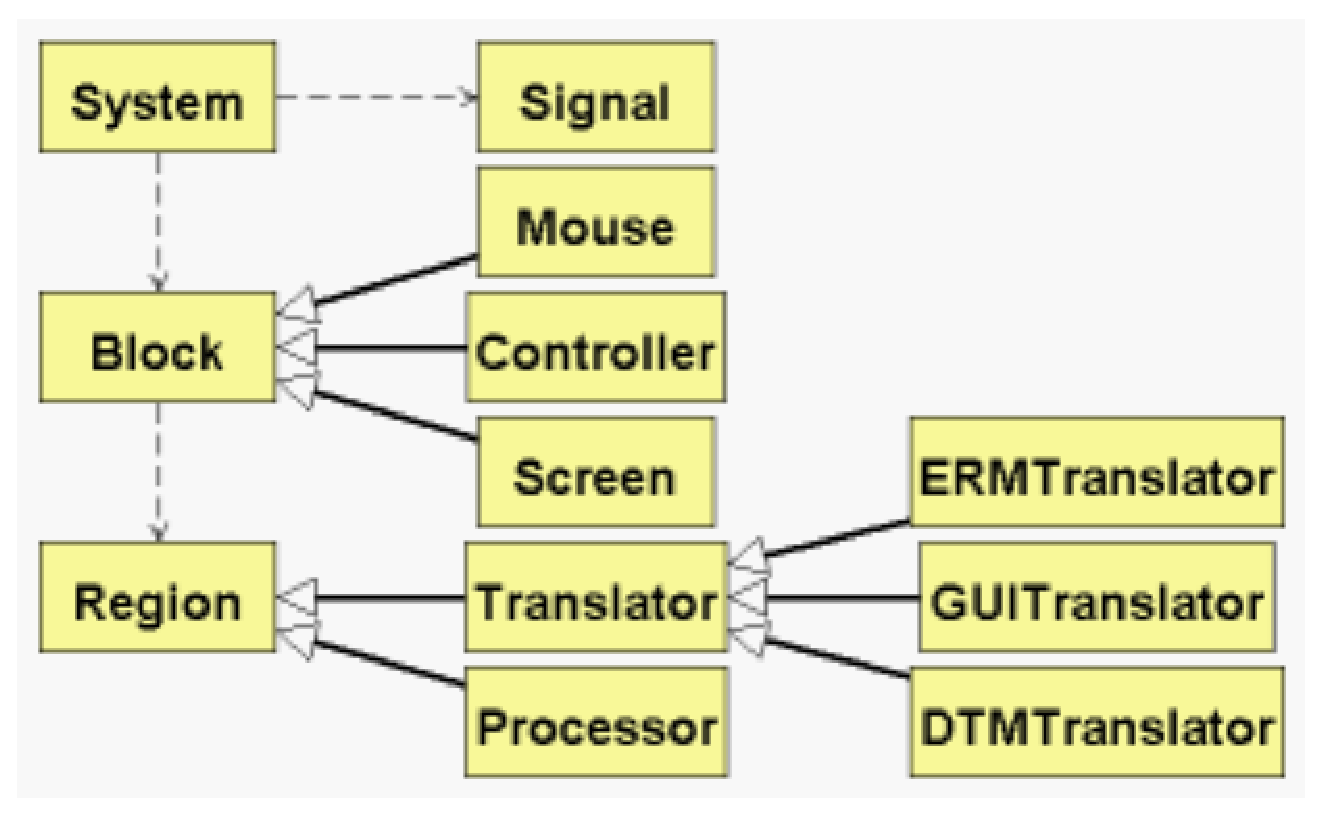
\includegraphics[scale=0.3]{vector/translator_classes.eps}
        \caption{Translator Classes in a UML Class Diagram}
        \label{translator_classes_figure}
    \end{center}
\end{figure}

Every system has exactly one domain model but communication models of arbitrary
type can be added anytime (figure \ref{translator_accessing_models_figure}). Every
translator knows only how to translate between the domain model and a special
communication model. Direct translation between communication models is forbidden
as it would break the flexibility of the whole framework. In other words,
translations always have to be done \emph{via} the domain model.

\begin{figure}[ht]
    \begin{center}
        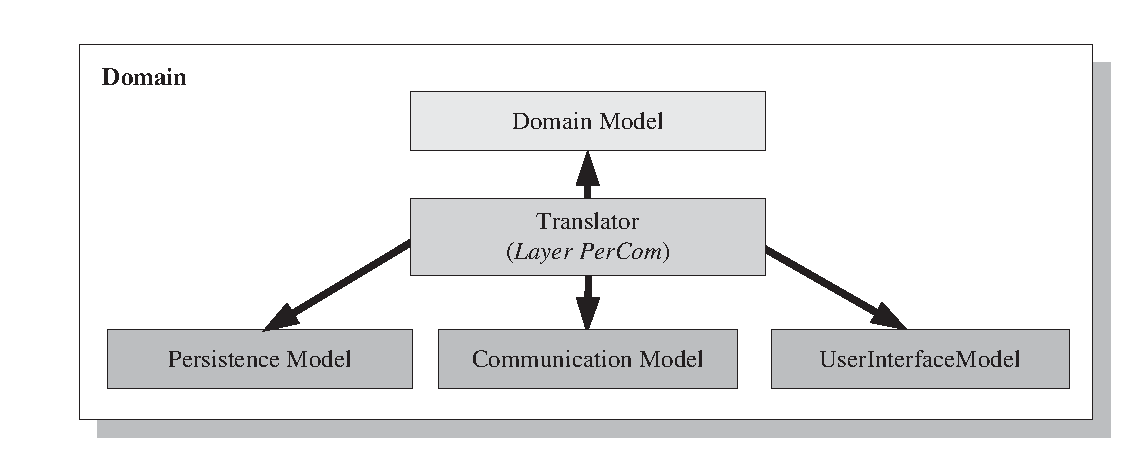
\includegraphics[scale=0.4]{vector/translator_accessing_models.eps}
        \caption{Translator accessing various Models}
        \label{translator_accessing_models_figure}
    \end{center}
\end{figure}


%
% $RCSfile: ontology_framework.tex,v $
%
% Copyright (c) 2001-2004. Christian Heller. All rights reserved.
%
% No copying, altering, distribution or any other actions concerning this
% document, except after explicit permission by the author!
% At some later point in time, this document is planned to be put under
% the GNU FDL license. For now, _everything_ is _restricted_ by the author.
%
% http://www.cybop.net
% - Cybernetics Oriented Programming -
%
% http://www.resmedicinae.org
% - Information in Medicine -
%
% @author Christian Heller <christian.heller@tuxtax.de>
%

\subsection{Ontology Framework}
\label{ontology_framework_heading}

When placing the translators of figure \ref{translator_classes_figure} into the
greater system architecture context, a \emph{System Ontology} as shown in
figure \ref{system_ontology_figure} may be retrieved. It contains the new
\emph{Translator} as sub class of \emph{Region}, input/ output devices as sub
class of \emph{Block}, \emph{Module} (\emph{Application}) and \emph{User} as sub
class of \emph{System} and further parts which are not the topic of this paper.
For the ease of understanding, the biological counterparts have been added on
the right side of the figure.\\
Specialized translators may be derived as sub class of the one shown in figure
\ref{system_ontology_figure}.

\begin{figure}[ht]
    \begin{center}
        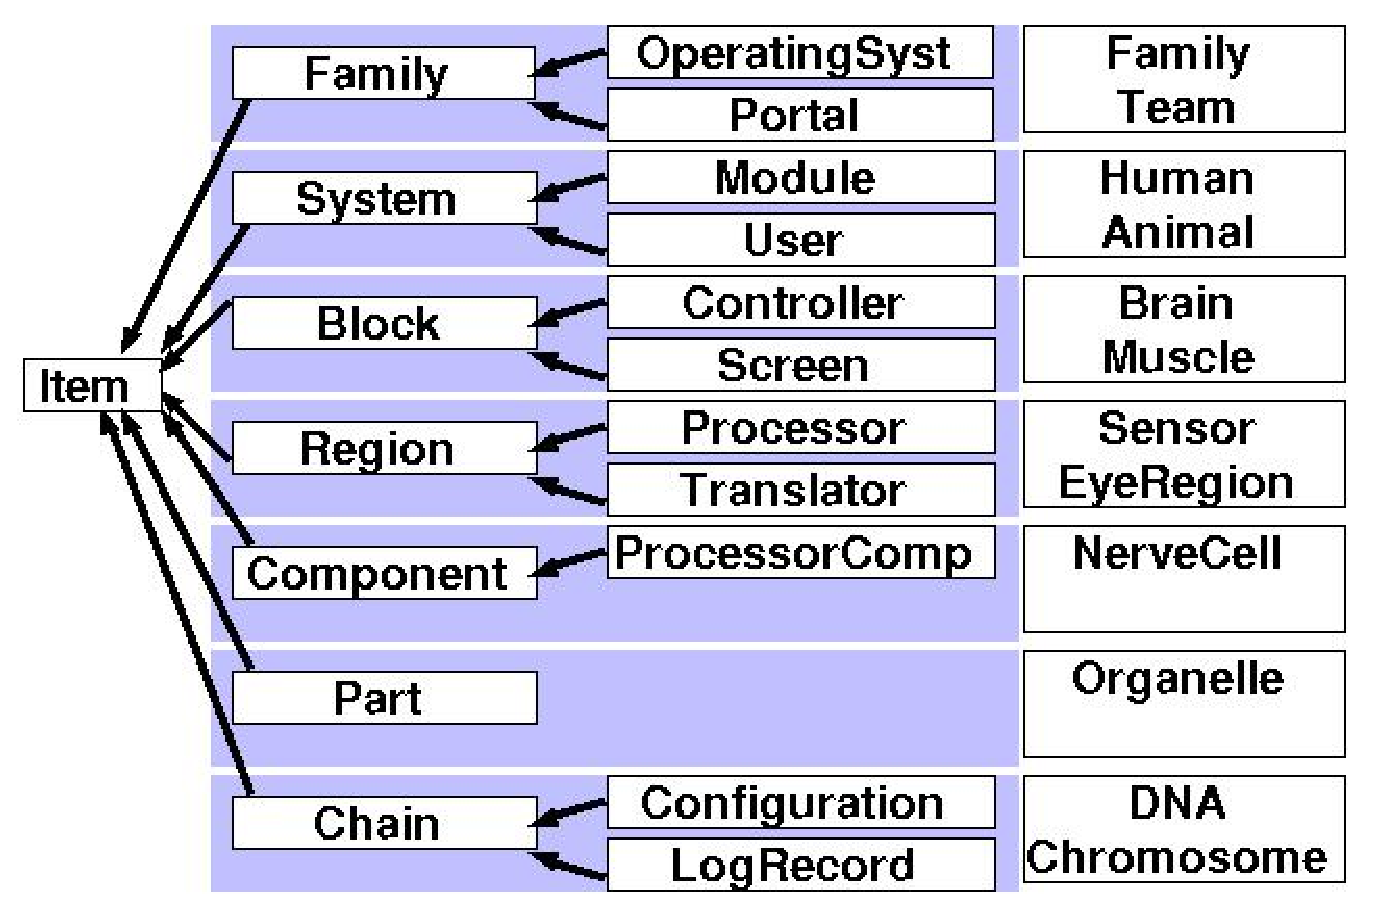
\includegraphics[scale=0.3]{vector/system_ontology.eps}
        \caption{System Ontology}
        \label{system_ontology_figure}
    \end{center}
\end{figure}

To complete the list of important ontology models, figure \ref{basic_ontology_figure}
gives an overview of language-integrated types (commonly called \emph{Primitives}).
And as a matter of fact: All typecasted programming languages already contain an
\emph{Ontology}!
These primitives represent the lowest layer in an ontology or in other words, the
last level of abstraction in software. That is also where \emph{Terminologies}
(that are mostly mentioned in conjunction with ontologies) come in. Basically,
these are sorted collections of terms (strings) but not further elaborated here.

\begin{figure}[ht]
    \begin{center}
        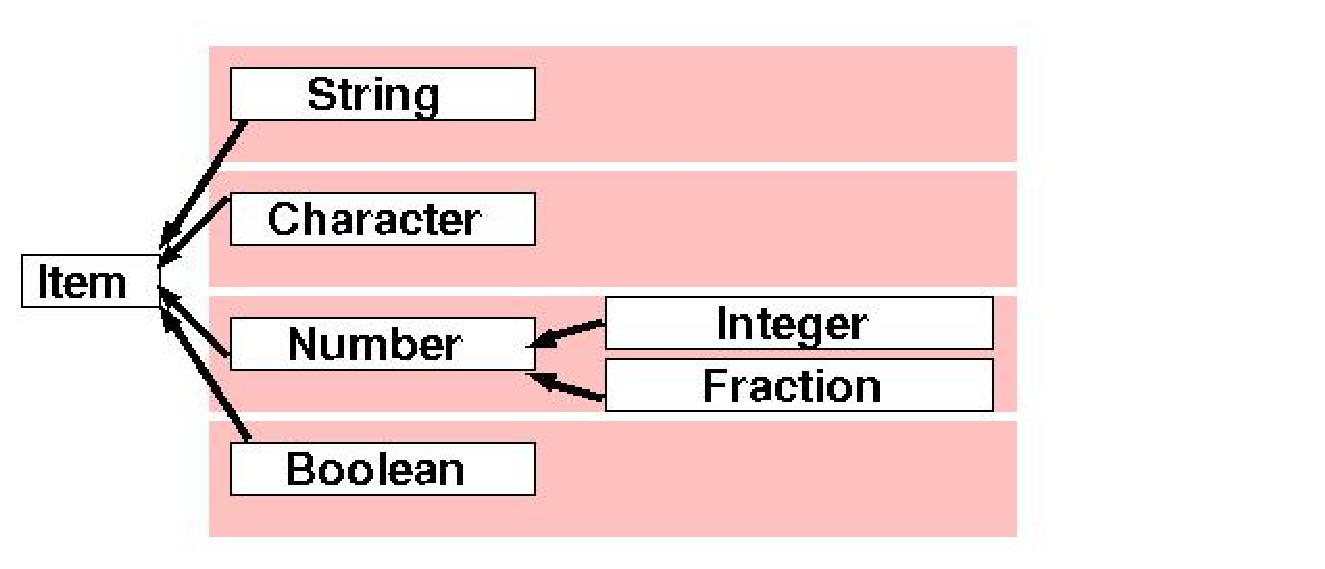
\includegraphics[scale=0.4]{vector/basic_ontology.eps}
        \caption{Basic (Language) Ontology}
        \label{basic_ontology_figure}
    \end{center}
\end{figure}

Putting the three ontologies \emph{Basic}, \emph{Model} and \emph{System} that were
introduced in this paper together, results in the CYBOP architecture of figure
\ref{ontology_framework_figure}. All ontologies base on the \emph{Language Ontology}.
A system built after the \emph{System Ontology} model (in this paper the example
of an \emph{Electronic Health Record} application) may access one ore more
\emph{Model Ontologies} (in the example the health record domain model).
All dependencies are unidirectional.

\begin{figure}[ht]
    \begin{center}
        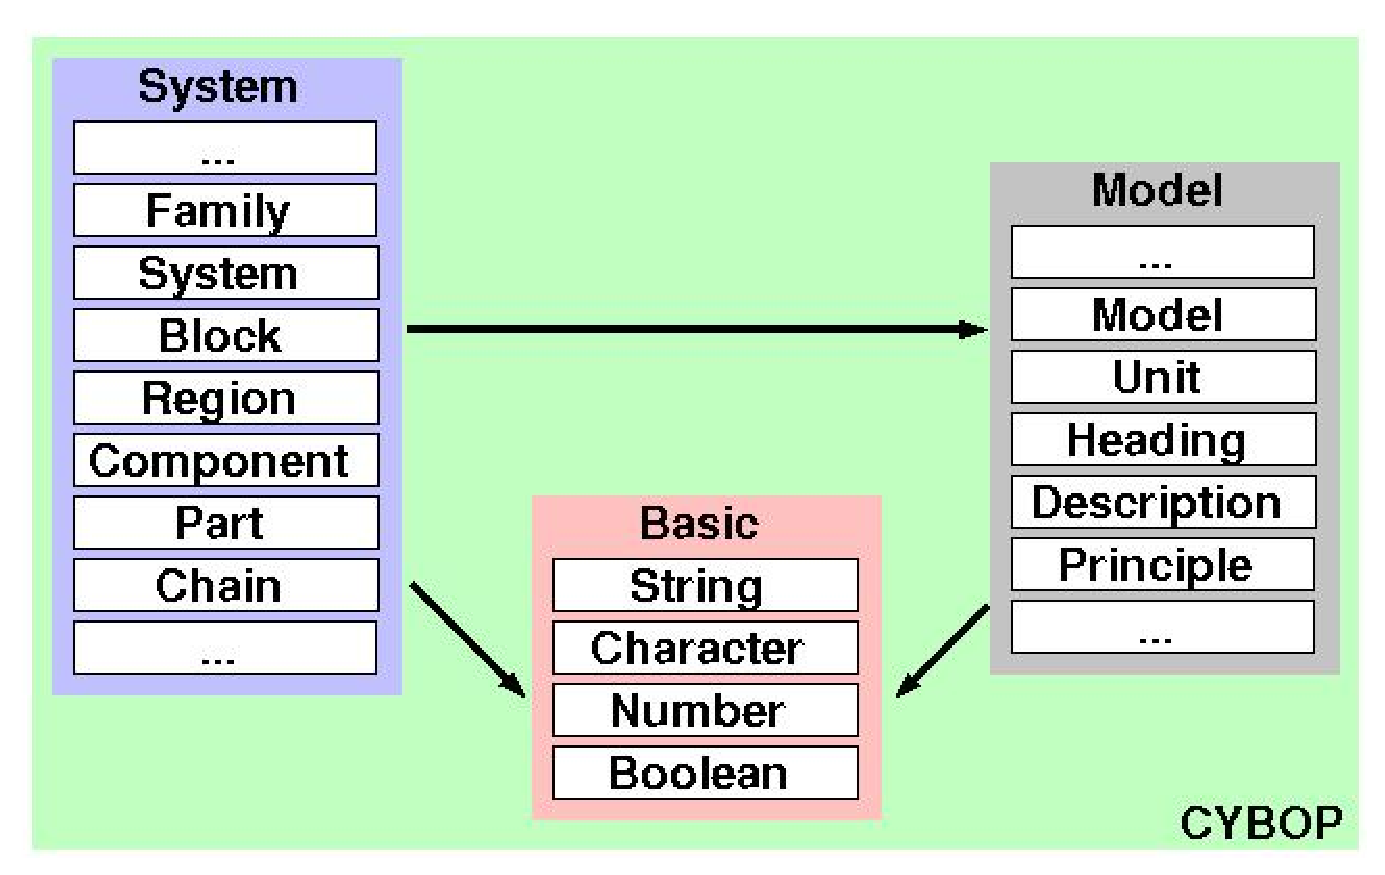
\includegraphics[scale=0.3]{vector/ontology_framework.eps}
        \caption{CYBOP Ontology Framework}
        \label{ontology_framework_figure}
    \end{center}
\end{figure}


%
% $RCSfile: consistency.tex,v $
%
% Copyright (c) 2001-2004. Christian Heller. All rights reserved.
%
% No copying, altering, distribution or any other actions concerning this
% document, except after explicit permission by the author!
% At some later point in time, this document is planned to be put under
% the GNU FDL license. For now, _everything_ is _restricted_ by the author.
%
% http://www.cybop.net
% - Cybernetics Oriented Programming -
%
% http://www.resmedicinae.org
% - Information in Medicine -
%
% @author Christian Heller <christian.heller@tuxtax.de>
%

\subsection{Consistency}
\label{consistency_heading}

The described models are highly flexible and extensible and absolutely transparent
to the user (developer). S/he will not know whether the current communication is
with the local file system, a database or a remote process on another machine.\\
However, this transparency causes a number of problems. Surely, the most common
question is how to ensure consistency, security and minimum redundance?
The following two paragraphs give an answer to the first part of this question
-- consistency and uniqueness of data sets. Maximizing security and minimizing
redundancy have to be analysed in future works.

%
% $RCSfile: object_id.tex,v $
%
% Copyright (c) 2001-2004. Christian Heller. All rights reserved.
%
% No copying, altering, distribution or any other actions concerning this
% document, except after explicit permission by the author!
% At some later point in time, this document is planned to be put under
% the GNU FDL license. For now, _everything_ is _restricted_ by the author.
%
% http://www.cybop.net
% - Cybernetics Oriented Programming -
%
% http://www.resmedicinae.org
% - Information in Medicine -
%
% @author Christian Heller <christian.heller@tuxtax.de>
%

\subsubsection{Object ID (OID)}
\label{object_id_heading}

Most database systems provide an own algorithm to generate primary keys for the
tables. But the applications that use our communication architecture shall also
be able to work if a database server is not reachable, e.g. due to a network
failure. Thats why the keys are generated locally, by each application.
Based on the assumption that every host in a network has a network card, it thereby
has a unique internet address. This number is concatinated with an exact time stamp
(nanoseconds). That is why the OID is unique in the global network and unique in
time.\\
The proposed approach uses the OID as file name for local storage and the same
OID as primary key in the main table of the database. Therewith, both models can
be mapped to each other. Of course, it is necessary to avoid overwriting of new
data in the database. If, for example, a network connection is cut and a little
later, one wants to get data from the local files and write them up in the restored
central database, it has to be made sure that nobody else has modified the data
during the offline-time. That is why there is another technique to ensure this
-- the time stamp.


%
% $RCSfile: time_stamp.tex,v $
%
% Copyright (c) 2001-2004. Christian Heller. All rights reserved.
%
% No copying, altering, distribution or any other actions concerning this
% document, except after explicit permission by the author!
% At some later point in time, this document is planned to be put under
% the GNU FDL license. For now, _everything_ is _restricted_ by the author.
%
% http://www.cybop.net
% - Cybernetics Oriented Programming -
%
% http://www.resmedicinae.org
% - Information in Medicine -
%
% @author Christian Heller <christian.heller@tuxtax.de>
%

\subsubsection{Time Stamp}
\label{time_stamp_heading}

Most database developers will know this technique. Each table has a separate
column for storing the time at which the data were written into this table.
If someone requests information from the database, the time stamp is delivered
as well. After modifying the data, they have to be written back into the database.
At this time, both timestamps (the one in the database table and the one delivered
before) are compared. If there is a difference, the data were modified by another
user. Then, one has to care about the update without overwriting the new data in
the table.






    %
% $RCSfile: physical_architecture.tex,v $
%
% Copyright (C) 2002-2008. Christian Heller.
%
% Permission is granted to copy, distribute and/or modify this document
% under the terms of the GNU Free Documentation License, Version 1.1 or
% any later version published by the Free Software Foundation; with no
% Invariant Sections, with no Front-Cover Texts and with no Back-Cover
% Texts. A copy of the license is included in the section entitled
% "GNU Free Documentation License".
%
% http://www.cybop.net
% - Cybernetics Oriented Programming -
%
% http://www.resmedicinae.org
% - Information in Medicine -
%
% Version: $Revision: 1.1 $ $Date: 2008-08-19 20:41:08 $ $Author: christian $
% Authors: Christian Heller <christian.heller@tuxtax.de>
%

\chapter{Physical Architecture}
\label{physical_architecture_heading}
\index{Physical Architecture}
\index{Communication}
\index{Autonomous Systems}
\index{Interaction and Cooperation}
\index{Technical Systems}
\index{Computer}
\index{Client}
\index{Server}
\index{Communication Partners}
\index{System Constellations}
\index{Communication Languages}
\index{Information Technology Environment}
\index{IT}

\begin{flushright}
    \textsl{Simplicity is the Result of Maturity.}\\
    \textsc{Johann Christoph Friedrich von Schiller}
\end{flushright}

Software provides the functionality through which robots act and computers
represent and process information. Both are special kinds of machines which only
get useful for humans if they can be controlled and communicated with.
\emph{Communication} is an essential ability for almost any kind of system.
\emph{Autonomous} systems exist and may well be useful, but is it nearly always
the \emph{Interaction} and \emph{Cooperation} that makes technical systems (from
now on called \emph{Computer} in this work) so interesting and helpful to humans.

In many cases, systems are limited to one role: \emph{Client} or \emph{Server}.
Clients ask questions which servers answer. But both are able to send as well
as to receive information. One-way communication without any feedback is rarely
useful. Besides the mentioned client- and server-, there are other roles that a
computer system can take on when talking with so-called
\emph{Communication Partners}.

The following sections will stepwise build up- and briefly investigate some
examples of well-known system constellations and possible communication
languages that are commonly used in a general \emph{Information Technology}
(IT) environment. Because physical systems and their interactions are
considered without any knowledge about their inside, one also talks of this as
the \emph{Physical Architecture} of an IT environment. Its understanding is
important for later reflections on the inner architecture of software systems
(chapter \ref{logical_architecture_heading}). Also will chapter
\ref{state_and_logic_heading} come back to system communication principles and
introduce a translator architecture for universal communication.

%
% $RCSfile: process.tex,v $
%
% Copyright (C) 2002-2008. Christian Heller.
%
% Permission is granted to copy, distribute and/or modify this document
% under the terms of the GNU Free Documentation License, Version 1.1 or
% any later version published by the Free Software Foundation; with no
% Invariant Sections, with no Front-Cover Texts and with no Back-Cover
% Texts. A copy of the license is included in the section entitled
% "GNU Free Documentation License".
%
% http://www.cybop.net
% - Cybernetics Oriented Programming -
%
% http://www.resmedicinae.org
% - Information in Medicine -
%
% Version: $Revision: 1.1 $ $Date: 2008-08-19 20:41:08 $ $Author: christian $
% Authors: Christian Heller <christian.heller@tuxtax.de>
%

\section{Process}
\label{process_heading}
\index{Process}
\index{Resource Grouping}
\index{Execution}
\index{Address Space}
\index{Thread of Execution}
\index{Central Processing Unit}
\index{CPU}
\index{Program Counter}
\index{Registers}
\index{Stack}
\index{Abstract System Concepts}
\index{Operating System}
\index{OS}
\index{Session}
\index{Process Group}
\index{Job}
\index{System}
\index{Application}
\index{Task}
\index{Lightweight Process}
\index{Work Queue}
\index{Task Farm}
\index{Task Bag}

The most common word used to describe a running computer program is
\emph{Process}. Tanenbaum \cite{tanenbaum2001} defines it as an abstract model
based on two independent concepts: \emph{Resource Grouping} (space) and
\emph{Execution} (time).

He writes that \emph{Resource Grouping} meant that a process had an address
space containing program text and data, as well as other resources. A
\emph{Thread of Execution}, on the other hand, were the entity scheduled for
execution on the \emph{Central Processing Unit} (CPU). It had a program counter
(keeping track of which instruction to execute next), registers (holding its
current working variables) and a stack (containing the execution history, with
one frame for each procedure called but not yet returned from). Although a
thread would have to execute in some process, the thread and its process were
different concepts and could be treated separately.

A slightly different explanation is given in \cite{iseries}:

\begin{quote}
    A thread is the path a program takes while it runs, the steps it performs,
    and the order in which it performs the steps. A thread runs code from its
    starting location in an ordered, predefined sequence for a given set of
    inputs. The term \emph{Thread} is shorthand for \emph{Thread of Control}.
    (One) can use multiple threads to improve application performance by
    running different application tasks simultaneously.
\end{quote}

\begin{table}[ht]
    \begin{center}
        \begin{footnotesize}
        \begin{tabular}{| p{25mm} | p{45mm} | p{35mm} |}
            \hline
            \textbf{Abstract Concept} & \textbf{Explanation} & \textbf{Synonyms}\\
            \hline
            Session & Bundle of processes of one user &\\
            \hline
            Process Group & Collection of one or more processes & Job\\
            \hline
            Process & Container for related Resources & System, Application, Task\\
            \hline
            Thread & Schedulable Entity & Lightweight Process\\
            \hline
        \end{tabular}
        \end{footnotesize}
        \caption{Systematics of Abstract System Concepts}
        \label{concepts_table}
    \end{center}
\end{table}

There are other abstract concepts which are of importance, especially in an
\emph{Operating System} (OS) context. A terminal in the \emph{Linux} OS
\cite{johnson}, for example, may control a \emph{Session} consisting of
\emph{Process Groups} which in turn contain many \emph{Processes} providing
resources for the threads running in them. Table \ref{concepts_table} shows one
possible systematics of these concepts.

Some ambiguities exist, however. The term \emph{Job} which, some decades ago,
still stood for a program or set of programs, is nowadays used to label a
process group in \emph{Windows 2000} \cite[p. 7, 796]{tanenbaum2001} and
similarly in \emph{Linux} \cite[p. 125, 237]{johnson}. The notion of a
\emph{Task} is sometimes used equivalent to thread \cite{daene}, but other
times refers to a process or even process group \cite[p. 113]{johnson}.
Additionally, some sources use the term in the meaning of a signal or event
belonging to a work queue called \emph{Task Farm} or \emph{Task Bag}
\cite[p. 548, 606]{tanenbaum1999}.

This document uses the more general word \emph{System} to write about a process
that manages the input, storage, processing and output of data in a computer.
This is contrary to some other works which mean a whole computer, including its
hardware and software programs running on it, when talking about systems. In
the understanding of this work, once again, a \emph{System} is a \emph{Process}
(software system) running on a \emph{Computer} (hardware system).

%
% $RCSfile: application_server.tex,v $
%
% Copyright (C) 2002-2008. Christian Heller.
%
% Permission is granted to copy, distribute and/or modify this document
% under the terms of the GNU Free Documentation License, Version 1.1 or
% any later version published by the Free Software Foundation; with no
% Invariant Sections, with no Front-Cover Texts and with no Back-Cover
% Texts. A copy of the license is included in the section entitled
% "GNU Free Documentation License".
%
% http://www.cybop.net
% - Cybernetics Oriented Programming -
%
% http://www.resmedicinae.org
% - Information in Medicine -
%
% Version: $Revision: 1.1 $ $Date: 2008-08-19 20:41:05 $ $Author: christian $
% Authors: Christian Heller <christian.heller@tuxtax.de>
%

\section{Application Server}
\label{application_server_heading}
\index{Application Server}
\index{Presentation Clients}
\index{Standalone Systems}
\index{Operating System}
\index{OS}
\index{Layers}
\index{Tier}
\index{1 Tier}
\index{n Tier}
\index{Server Process}
\index{Server}
\index{Client}

One well-known system, nowadays, is the \emph{Application Server}. The name
implies that this system is to \emph{serve} other systems, so-called
\emph{Presentation Clients} (section \ref{presentation_client_heading}). It may
be programmed in languages like \emph{Java}, \emph{Python}, \emph{Smalltalk},
\emph{C++}, \emph{C} or others more.

On the other hand, there are systems running all by themselves, without any
access to/ from another system -- so-called \emph{Standalone Systems}. In
reality, they hardly exist since most applications run in a surrounding
\emph{Operating System} (OS) and are thus not really \emph{alone}. An OS may be
called \emph{standalone} but mostly, even that consists of a number of sub
processes solving background tasks. That is why the name \emph{standalone} is
used when one wants to place emphasis on the system itself, neglecting its
communication with others.

Many kinds of application servers exist. Multiple services are offered by them,
for example storage or persistence handling but also application- and domain
specific functionality. A healthcare environment, as example, may contain several
servers, each fulfilling one task such as person identification, resource access
decision, image access and so on -- just like people in real life have abilities
and professions.

Systems of an IT environment are structured into so-called \emph{Layers},
another name for which is \emph{Tier}. The application server alone represents
a \emph{1 Tier} environment. The more systems of different type (presentation
client, application server, database server) are added to an environment, the
more tiers are added. For that reason, distributed client-server environments
are called \emph{n Tier}.

When people talk about a \emph{Server}, they very often mean a \emph{Computer}
on which a \emph{Server Process} is running. This is neither completely wrong nor
absolutely correct. A computer can run many different processes, only some of
which may be servers. Hence, the computer can act as \emph{Server} but also as
\emph{Client}, at the same time.

%
% $RCSfile: database_server.tex,v $
%
% Copyright (C) 2002-2008. Christian Heller.
%
% Permission is granted to copy, distribute and/or modify this document
% under the terms of the GNU Free Documentation License, Version 1.1 or
% any later version published by the Free Software Foundation; with no
% Invariant Sections, with no Front-Cover Texts and with no Back-Cover
% Texts. A copy of the license is included in the section entitled
% "GNU Free Documentation License".
%
% http://www.cybop.net
% - Cybernetics Oriented Programming -
%
% http://www.resmedicinae.org
% - Information in Medicine -
%
% Version: $Revision: 1.1 $ $Date: 2008-08-19 20:41:06 $ $Author: christian $
% Authors: Christian Heller <christian.heller@tuxtax.de>
%

\section{Database Server}
\label{database_server_heading}
\index{Database Server}
\index{Database Management System}
\index{DBMS}
\index{Database}
\index{DB}
\index{2 Tiers}
\index{Persistent Data}
\index{Transient Data}
\index{Querying}
\index{Transaction Handling}
\index{Locking}
\index{Hierarchical DBMS}
\index{Network DBMS}
\index{Relational DBMS}
\index{RDBMS}
\index{Object-Relational DBMS}
\index{ORDBMS}
\index{Object-Oriented DBMS}
\index{OODBMS}
\index{Data Definition Language}
\index{DDL}
\index{Structured Query Language}
\index{SQL}
\index{Object-Relational DBMS}
\index{Object-Oriented Model}
\index{OOM}
\index{Entity-Relationship Model}
\index{ERM}
\index{Object Query Language}
\index{OQL}
\index{Middleware}
\index{Java Database Connectivity}
\index{JDBC}
\index{Open Database Connectivity}
\index{ODBC}
\index{Enterprise Java Beans}
\index{EJB}
\index{Business Objects}
\index{BO}

Another popular kind of server system, besides the application server, is the
\emph{Database Server}, also called \emph{Database Management System} (DBMS).
It manages structured data called a \emph{Database} (DB) and serves clients
with \emph{persistent} data. The arrow in figure \ref{database_figure} points
in the direction into which the application server sends its queries to the
database server, in order to retrieve data. Example DBMS representatives are
\emph{PostgreSQL}, \emph{MySQL}, \emph{DB2}, \emph{ORACLE}, \emph{ObjectStore},
\emph{POET} or \emph{Versant}.

\begin{figure}[ht]
    \begin{center}
        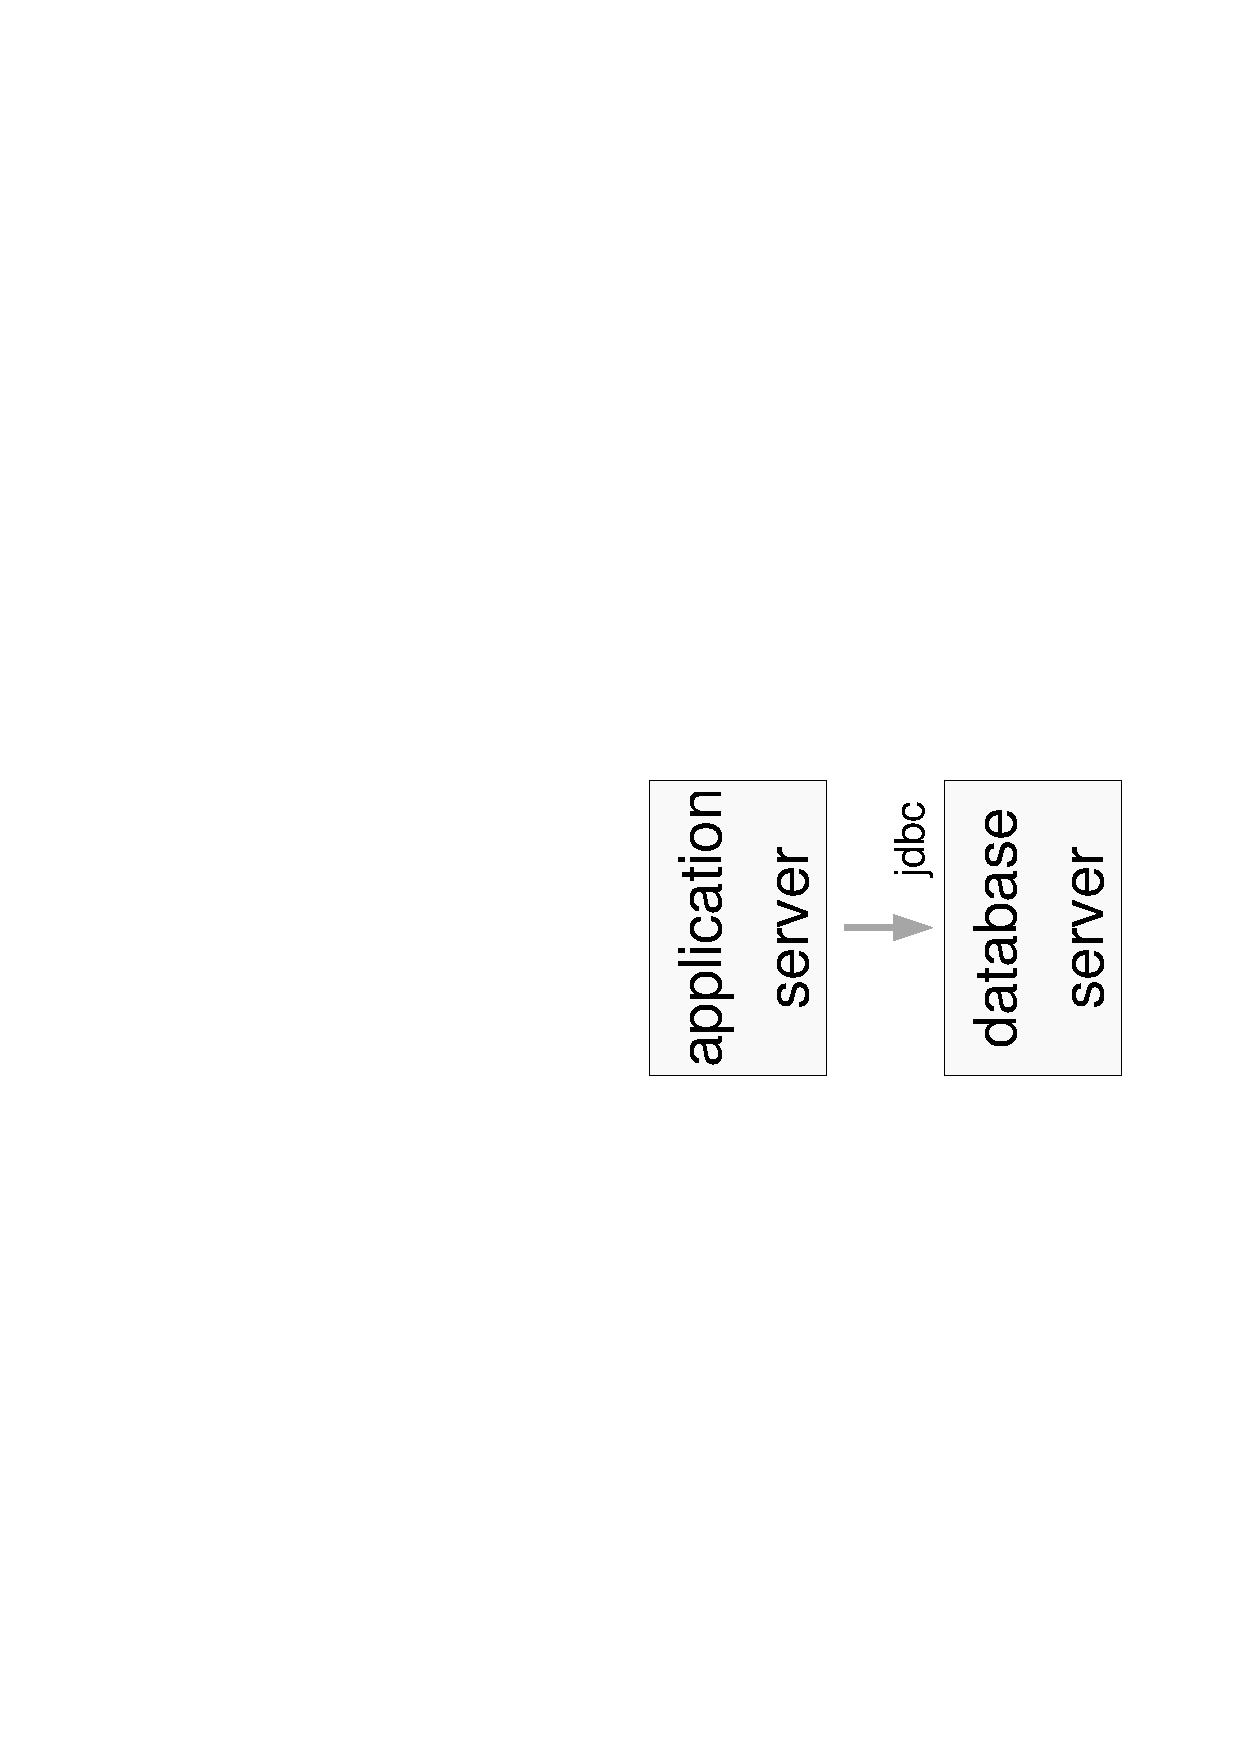
\includegraphics[scale=0.3,angle=-90]{graphic/database.pdf}
        \caption{Database Server (2 Tiers)}
        \label{database_figure}
    \end{center}
\end{figure}

\emph{Persistent Data} are those that live longer than the system working on them.
Very often, this is domain-specific- but also configuration information. These
are stored in a filesystem or database \cite{zimmermann}. \emph{Transient Data},
on the other hand, is temporary information that a system holds during its
lifetime, to function correctly. They get destroyed together with the system
which created them.

Managing persistent data implies a number of quite complex tasks, the details of
which will not be part of this document. To these aspects of database servers
belong:

\begin{itemize}
    \item[-] Querying
    \item[-] Transaction Handling
    \item[-] Locking
\end{itemize}

Different types of database systems exist. The major ones are:

\begin{itemize}
    \item[-] \emph{Hierarchical and Network DBMS}
    \item[-] \emph{Relational DBMS} (RDBMS)
    \item[-] \emph{Object-Relational DBMS} (ORDBMS)
    \item[-] \emph{Object-Oriented DBMS} (OODBMS)
\end{itemize}

Hierarchical DBMS were the first (electronic) databases ever used. They managed
their data in tree structures, starting each access from the root node. Network
DBMS went one step further: data could be associated at will \cite[p. 128]{zimmermann}.
Relational DBMS are based on tabular data structures which can have relations.
They were the first to accomplish a true separation between application and data.
Special languages were created to define and query such data sources: The
\emph{Data Definition Language} (DDL) and the \emph{Structured Query Language}
(SQL). Object-Relational DBMS were to fill the semantic gap between
\emph{Object-Oriented Model} (OOM) and \emph{Entity-Relationship Model} (ERM)
structures. Their extensions introduced a number of user-defined data types.
Object-Oriented DBMS conclusively close the semantic gap between object-oriented
applications and data. Their programming interface is often integrated into a
framework. The new SQL-based \emph{Object Query Language} (OQL)
\cite[p. 138]{zimmermann} was created for them.

The communication between systems can be eased with special techniques. After
Tanenbaum \cite{tanenbaum2002}, these were often called \emph{Middleware} since
they are placed between a higher-level layer consisting of users and applications,
and a layer underneath consisting of operating systems. In the case of database
systems, one such mechanism is the \emph{Java Database Connectivity} (JDBC)
\cite{hamilton, klute}; another one the \emph{Open Database Connectivity}
(ODBC) \cite[p. 170, 177]{zimmermann}. They provide a common interface for many
different relational databases.

Another technique are \emph{Enterprise Java Beans} (EJB) and comparable mechanisms.
They represent so-called \emph{Business Objects} (BO) and hence actually belong
to the previous section describing application servers. However, the containers
in which EJBs live also contain functionality for persistence- and transaction
handling which is why they are mentioned here. Further documentation can be found
in the corresponding literature \cite{gruhn} and sources \cite{blueprints, java}.

%
% $RCSfile: presentation_client.tex,v $
%
% Copyright (C) 2002-2008. Christian Heller.
%
% Permission is granted to copy, distribute and/or modify this document
% under the terms of the GNU Free Documentation License, Version 1.1 or
% any later version published by the Free Software Foundation; with no
% Invariant Sections, with no Front-Cover Texts and with no Back-Cover
% Texts. A copy of the license is included in the section entitled
% "GNU Free Documentation License".
%
% http://www.cybop.net
% - Cybernetics Oriented Programming -
%
% http://www.resmedicinae.org
% - Information in Medicine -
%
% Version: $Revision: 1.1 $ $Date: 2008-08-19 20:41:08 $ $Author: christian $
% Authors: Christian Heller <christian.heller@tuxtax.de>
%

\section{Presentation Client}
\label{presentation_client_heading}
\index{Presentation Client}
\index{Client}
\index{3 Tiers}
\index{Remote Method Invocation}
\index{RMI}
\index{Remote Procedure Call}
\index{RPC}
\index{Thin Client}
\index{Fat Client}
\index{Rich Client}

A system is called \emph{Client} when it uses services of a server. Most modern
applications incorporate abilities to communicate with server systems which may
run on the same computer as the client or on a remote machine that has to be
accessed over network.

\begin{figure}[ht]
    \begin{center}
        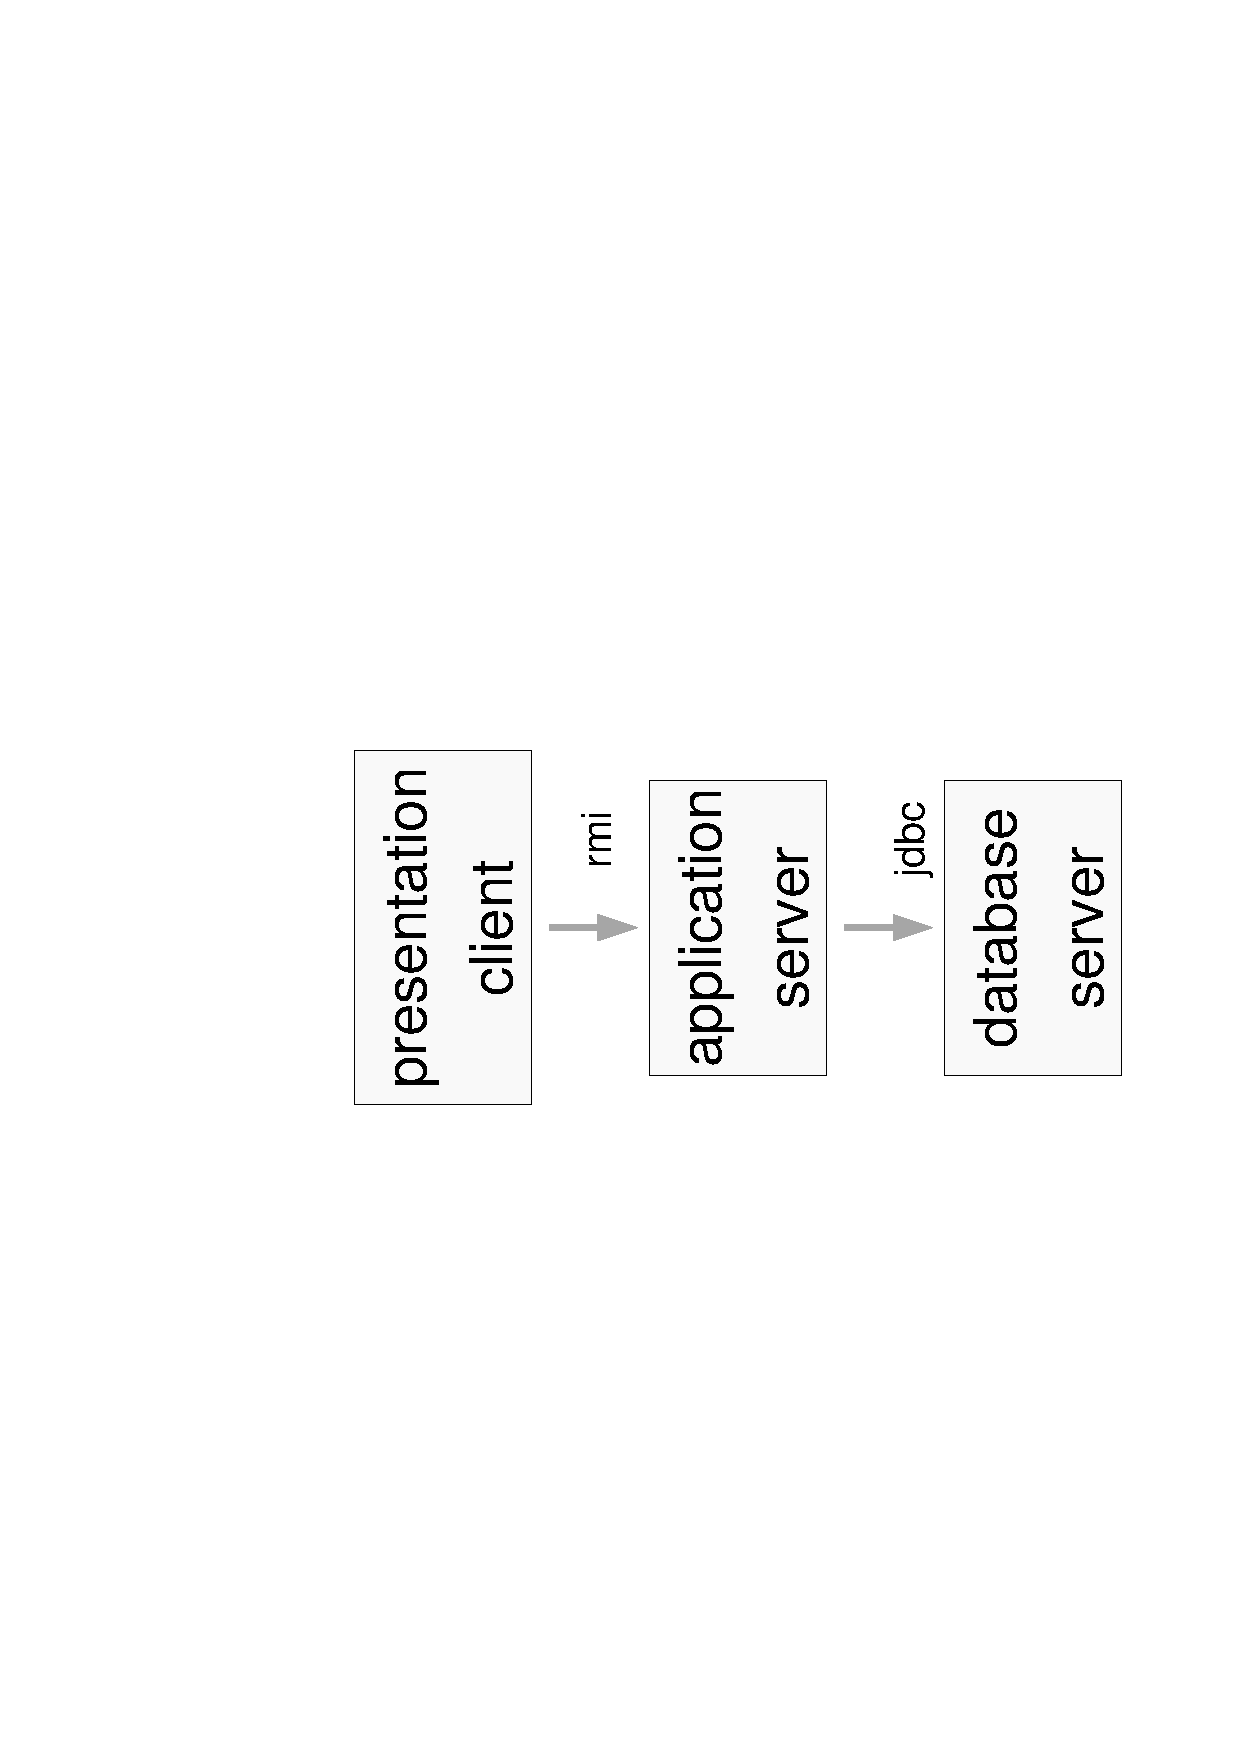
\includegraphics[scale=0.3,angle=-90]{graphic/client.pdf}
        \caption{Presentation Client (3 Tiers)}
        \label{client_figure}
    \end{center}
\end{figure}

But also clients can offer services as well as servers can use external services
and such become clients themselves. The application server in figure
\ref{database_figure} becomes a client when accessing the database system.
As can be seen -- \emph{Client} and \emph{Server} are quite arbitrary terms to
characterise systems.

Figure \ref{client_figure} illustrates the communication between a presentation
client and application server over network. Again, various mechanisms such as
\emph{Remote Method Invocation} (RMI), outside the Java world rather called
\emph{Remote Procedure Call} (RPC), exist to ease the way two remote systems
talk with one another.

Frequently, people distinguish between \emph{Thin Client} and \emph{Fat Client}
(the latter also called \emph{Rich Client}) \cite[p. 176]{zimmermann}. While a
thin client's task is nothing else than to display information coming from some
server, a fat client also takes over part of the business data processing which
is otherwise done by the server only.

%
% $RCSfile: web_client_and_server.tex,v $
%
% Copyright (C) 2002-2008. Christian Heller.
%
% Permission is granted to copy, distribute and/or modify this document
% under the terms of the GNU Free Documentation License, Version 1.1 or
% any later version published by the Free Software Foundation; with no
% Invariant Sections, with no Front-Cover Texts and with no Back-Cover
% Texts. A copy of the license is included in the section entitled
% "GNU Free Documentation License".
%
% http://www.cybop.net
% - Cybernetics Oriented Programming -
%
% http://www.resmedicinae.org
% - Information in Medicine -
%
% Version: $Revision: 1.1 $ $Date: 2008-08-19 20:41:09 $ $Author: christian $
% Authors: Christian Heller <christian.heller@tuxtax.de>
%

\section{Web Client and Server}
\label{web_client_and_server_heading}
\index{Web Client and Server}
\index{Internet}
\index{Web Server}
\index{Web Client}
\index{Web Browser}
\index{Applets}
\index{Servlets}
\index{Transfer Control Protocol}
\index{TCP}
\index{Internet Protocol}
\index{IP}
\index{Hypertext Transfer Protocol}
\index{HTTP}

With the emerge of the \emph{Internet}, several new kinds of services like
\emph{Email}, \emph{File Transfer}, \emph{Web} etc. became popular. The web
service allows information to be published in form of a \emph{Web Page}. Web
pages can be written in markup formats like \emph{Hypertext Markup Language}
(HTML) and \emph{Extensible Markup Language} (XML) or, using special tags, as
\emph{Java Server Pages-} (JSP) and \emph{PHP Hypertext Preprocessor-} (PHP)
instructions. Before being displayed, the latter two need to be translated by a
preprocessor inside the web server, into HTML.

\begin{figure}[ht]
    \begin{center}
        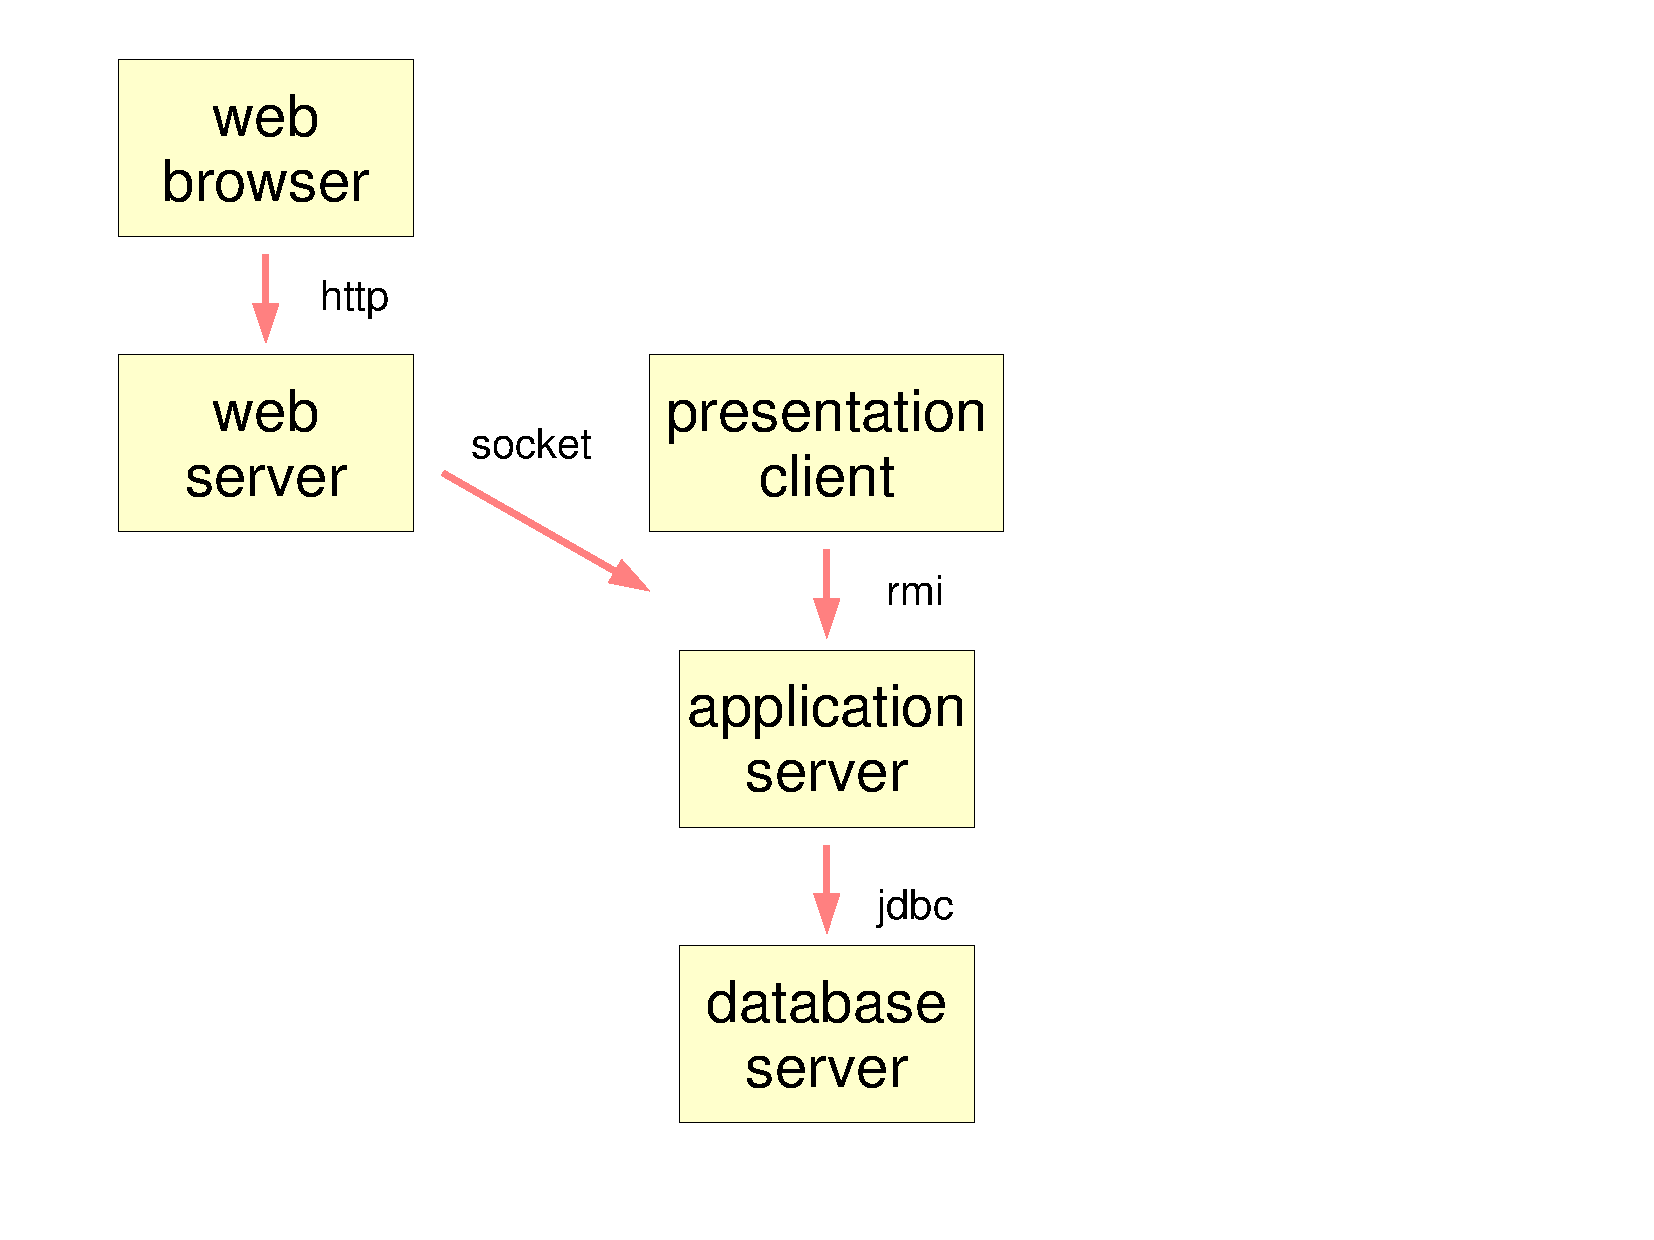
\includegraphics[scale=0.3,angle=-90]{graphic/web.pdf}
        \caption{Web Client and Server}
        \label{web_figure}
    \end{center}
\end{figure}

The principle as shown in figure \ref{web_figure} is easy: A \emph{Web Server}
stores web pages which can be accessed by clients called \emph{Web Browser}.
Browsers extract and translate (render) the (graphical) information given in
form of a web page and display them. But they are also able to handle actions
such as keyboard input or mouse click, and send these information back to the
web server.

Moreover, browsers can locally execute small programs called \emph{Applets}
which were downloaded from the web server. Their counterpart are \emph{Servlets}
which are executed in multiple threads on the web server, offering the actual
services.

Web communication is based on standards like the \emph{Transfer Control Protocol}/
\emph{Internet Protocol} (TCP/IP) and the \emph{Hypertext Transfer Protocol}
(HTTP) \cite{tanenbaum2000}. Section \ref{systems_interconnection_heading} will
systematise them together with other standards for system interconnection. The
socket mechanism may be used to connect a web server to an application server.

Many other aspects are important when talking about internet services. There is
the issue of security, there is performance, user-friendliness and many more
which will not be discussed further here, since it would exceed the frame of
this work.

%
% $RCSfile: local_process.tex,v $
%
% Copyright (C) 2002-2008. Christian Heller.
%
% Permission is granted to copy, distribute and/or modify this document
% under the terms of the GNU Free Documentation License, Version 1.1 or
% any later version published by the Free Software Foundation; with no
% Invariant Sections, with no Front-Cover Texts and with no Back-Cover
% Texts. A copy of the license is included in the section entitled
% "GNU Free Documentation License".
%
% http://www.cybop.net
% - Cybernetics Oriented Programming -
%
% http://www.resmedicinae.org
% - Information in Medicine -
%
% Version: $Revision: 1.1 $ $Date: 2008-08-19 20:41:07 $ $Author: christian $
% Authors: Christian Heller <christian.heller@tuxtax.de>
%

\section{Local Process}
\label{local_process_heading}
\index{Local Process}
\index{Nodes}
\index{Daemon}
\index{Small Servers}
\index{Inter-Process Communication}
\index{IPC}
\index{Dynamic Data Exchange}
\index{DDE}
\index{Object Linking and Embedding}
\index{OLE}
\index{ActiveX}
\index{Component Object Model}
\index{COM}
\index{Java Message Service}
\index{JMS}
\index{Desktop Communication Protocol}
\index{DCOP}
\index{Bonobo}
\index{Pipes}

Not all software systems run on physically separated computers, also called
\emph{Nodes}. And not all communication happens over network. As well, one
\emph{Local Process} can talk to a second on the same machine (figure
\ref{local_figure}). In fact, all applications have this ability, at least for
talking with the surrounding operating system.

\begin{figure}[ht]
    \begin{center}
        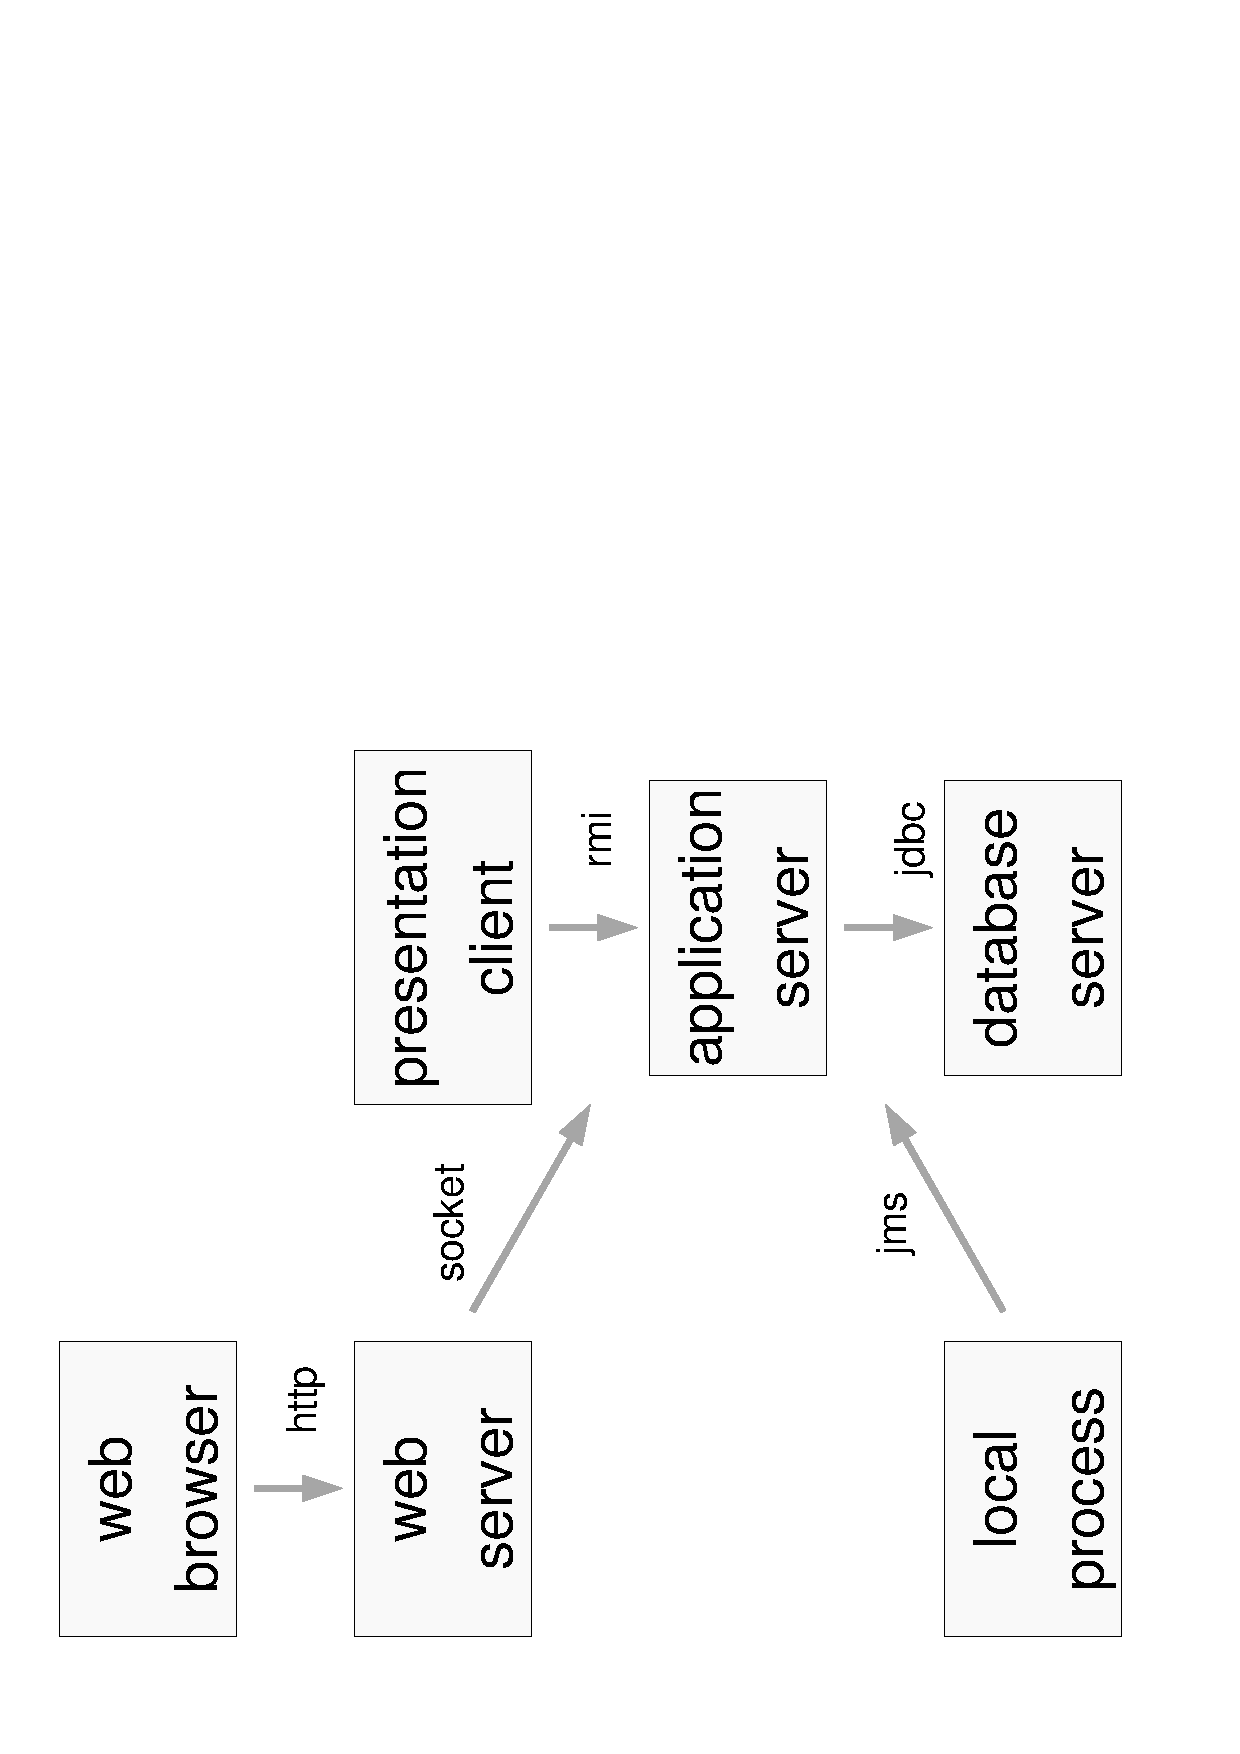
\includegraphics[scale=0.3,angle=-90]{graphic/local.pdf}
        \caption{Local Process}
        \label{local_figure}
    \end{center}
\end{figure}

Sometimes, local processes are needed by the operating system itself. Those are
running in the background then which is why they are often called \emph{Daemon}.
Because they offer special services, daemons are nothing else than small
servers. They fulfil tasks like managing all printing or email delivery of a
system, or similar things \cite[p. 74]{tanenbaum2001}.

Very often, it is useful to let local client applications talk with each other.
One part of a document (for instance a diagram) that was created by help of a
special application may want to get integrated into another document (for instance
a letter) which is edited by another application. A number of mechanisms were
created to solve this \emph{Inter-Process Communication} (IPC) task, for example:

\begin{itemize}
    \item[-] \emph{Dynamic Data Exchange} (DDE) \cite{ddefaq}
    \item[-] \emph{Object Linking and Embedding} (OLE/ OLE2) and \emph{ActiveX},
        both now based on the \emph{Component Object Model} (COM)
        \cite{zimmermann, gruhn}
    \item[-] \emph{Java Message Service} (JMS) \cite{java}
    \item[-] \emph{Desktop Communication Protocol} (DCOP) \cite{kde}
    \item[-] \emph{Bonobo} \cite{gnome}
    \item[-] \emph{Pipes} \cite{johnson, tanenbaum2001}
\end{itemize}

Although usually used for local communication (on the same node), some of these
also function over network. Again, this document will not discuss their inside
functionality. Plenty of books were written about that.

%
% $RCSfile: human_user.tex,v $
%
% Copyright (C) 2002-2008. Christian Heller.
%
% Permission is granted to copy, distribute and/or modify this document
% under the terms of the GNU Free Documentation License, Version 1.1 or
% any later version published by the Free Software Foundation; with no
% Invariant Sections, with no Front-Cover Texts and with no Back-Cover
% Texts. A copy of the license is included in the section entitled
% "GNU Free Documentation License".
%
% http://www.cybop.net
% - Cybernetics Oriented Programming -
%
% http://www.resmedicinae.org
% - Information in Medicine -
%
% Version: $Revision: 1.1 $ $Date: 2008-08-19 20:41:07 $ $Author: christian $
% Authors: Christian Heller <christian.heller@tuxtax.de>
%

\section{Human User}
\label{human_user_heading}
\index{Human User}
\index{Textual User Interface}
\index{TUI}
\index{Graphical User Interface}
\index{GUI}
\index{Human-Computer Interaction}
\index{HCI}

One system that needs special consideration is the \emph{Human User}. In the
first instance, it can be seen as normal system that is able to communicate
with other humans but also with artificial software systems running on machines
such as computers (figure \ref{user_figure}).

\begin{figure}[ht]
    \begin{center}
        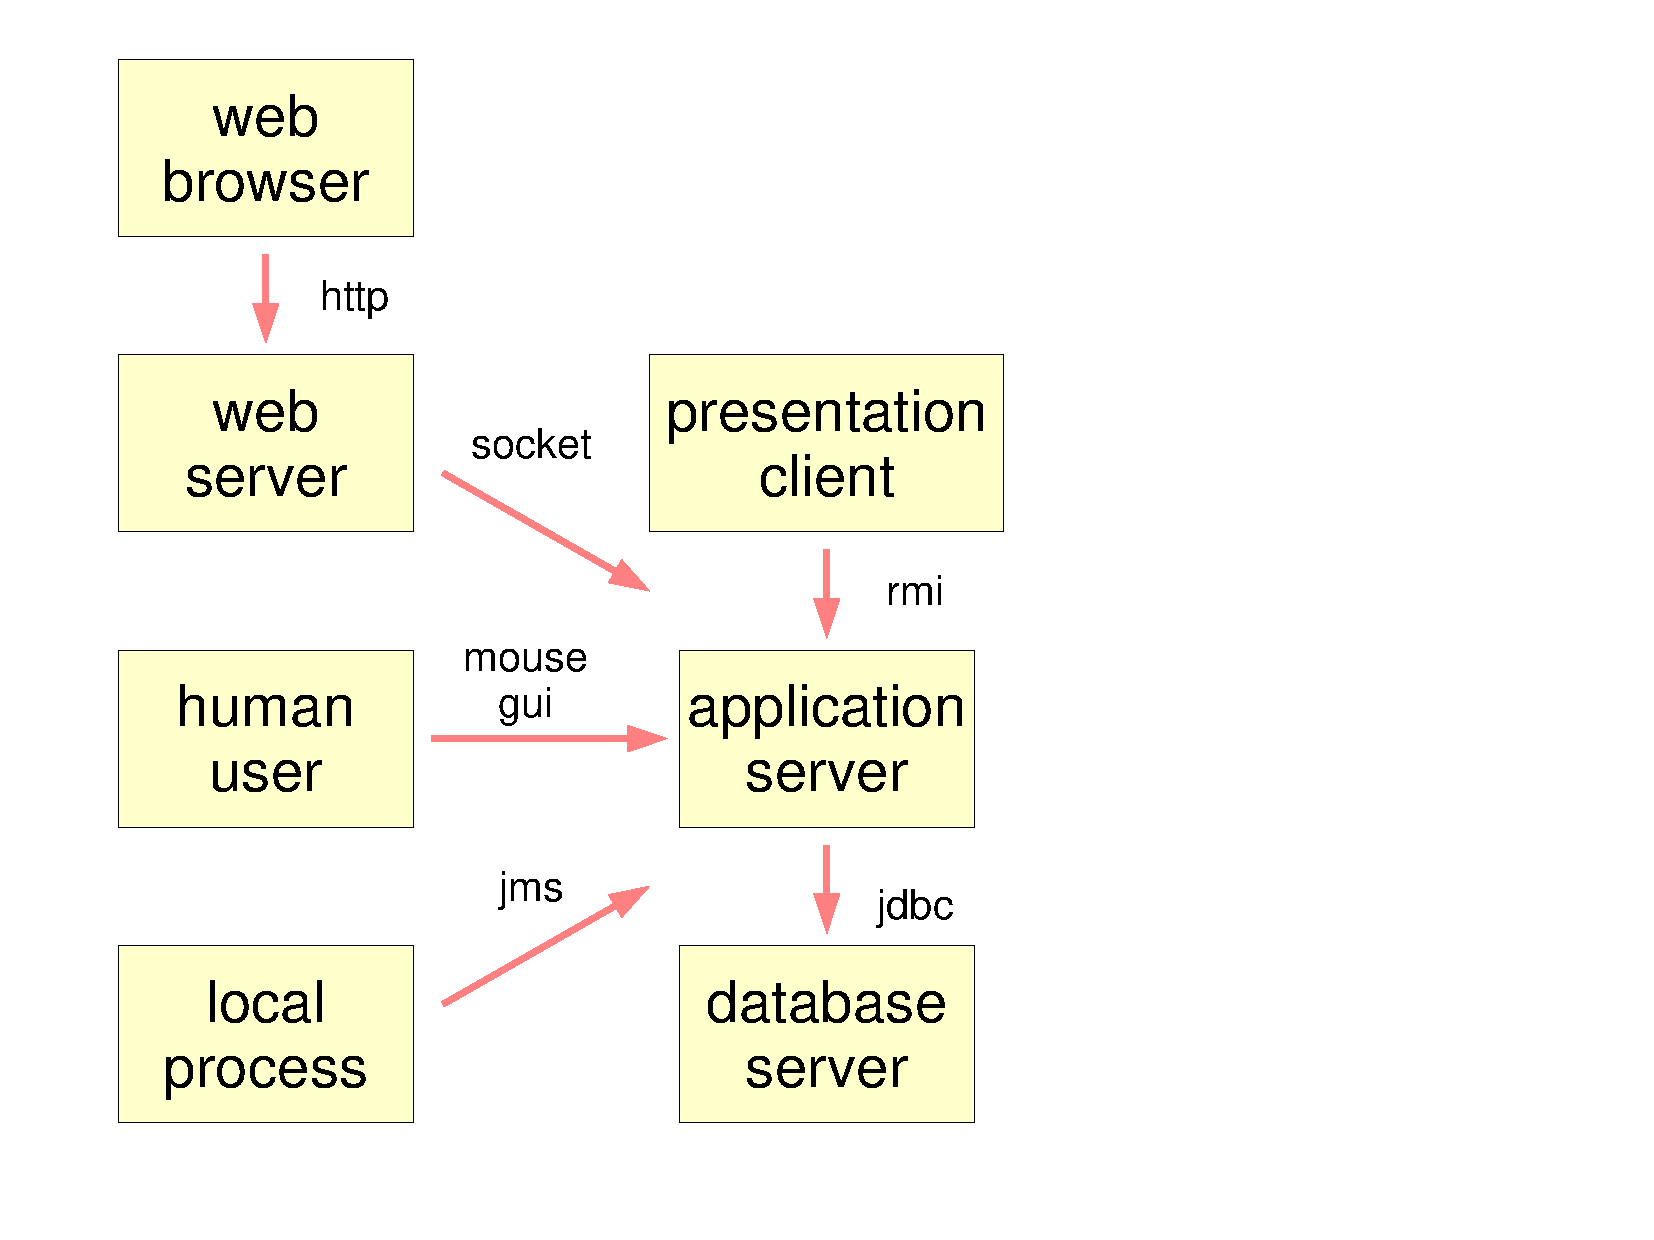
\includegraphics[scale=0.3,angle=-90]{graphic/user.pdf}
        \caption{Human User}
        \label{user_figure}
    \end{center}
\end{figure}

At the second view, one realises that due to the difference in construction,
human systems rely on other kinds of communication signals. While network cards
are usually enough for two computers to exchange data, additional input/ output
devices are needed to let human beings and computers talk to each other. To these
devices count: \emph{Keyboard}, \emph{Mouse}, \emph{Screen}, \emph{Printer} and
many more. They are made to suit the five human senses, that is to generate and
understand optical, acoustical, mechanical and similar signals.

The optical information displayed on a screen is often systematised into
character-based \emph{Textual User Interface} (TUI) and window-based
\emph{Graphical User Interface} (GUI).

The scientific subject dealing with those issues in more detail is called
\emph{Human-Computer Interaction} (HCI). One working definition given in
\cite{sigchi} states:

\begin{quote}
    Human-computer interaction is a discipline concerned with the design,
    evaluation and implementation of interactive computing systems for human
    use and with the study of major phenomena surrounding them.
\end{quote}

%
% $RCSfile: peer_node.tex,v $
%
% Copyright (C) 2002-2008. Christian Heller.
%
% Permission is granted to copy, distribute and/or modify this document
% under the terms of the GNU Free Documentation License, Version 1.1 or
% any later version published by the Free Software Foundation; with no
% Invariant Sections, with no Front-Cover Texts and with no Back-Cover
% Texts. A copy of the license is included in the section entitled
% "GNU Free Documentation License".
%
% http://www.cybop.net
% - Cybernetics Oriented Programming -
%
% http://www.resmedicinae.org
% - Information in Medicine -
%
% Version: $Revision: 1.1 $ $Date: 2008-08-19 20:41:08 $ $Author: christian $
% Authors: Christian Heller <christian.heller@tuxtax.de>
%

\section{Peer Node}
\label{peer_node_heading}
\index{Peer Node}
\index{Distributed System}
\index{Distributed Computing Environment}
\index{DCE}
\index{c/s}
\index{Peer-to-Peer}
\index{P2P}
\index{Client}
\index{Server}
\index{Freenet}
\index{Gnutella}
\index{BitTorrent}
\index{eDonkey}
\index{FastTrack}
\index{Napster}

Tanenbaum and Steen \cite{tanenbaum2002} define a \emph{Distributed System} as
\textit{a collection of independent computers that appear to its users as a
single coherent system}. With \emph{System} referring to a process rather than
only hardware, as defined in section \ref{process_heading}, it seems appropriate
to rephrase and use this for the definition of a general
\emph{Distributed Computing Environment} (DCE):

\begin{quote}
    A distributed computing environment consists of at least two systems that
    work together over a network but run on independent computer hardware (nodes).
\end{quote}

\begin{figure}[ht]
    \begin{center}
        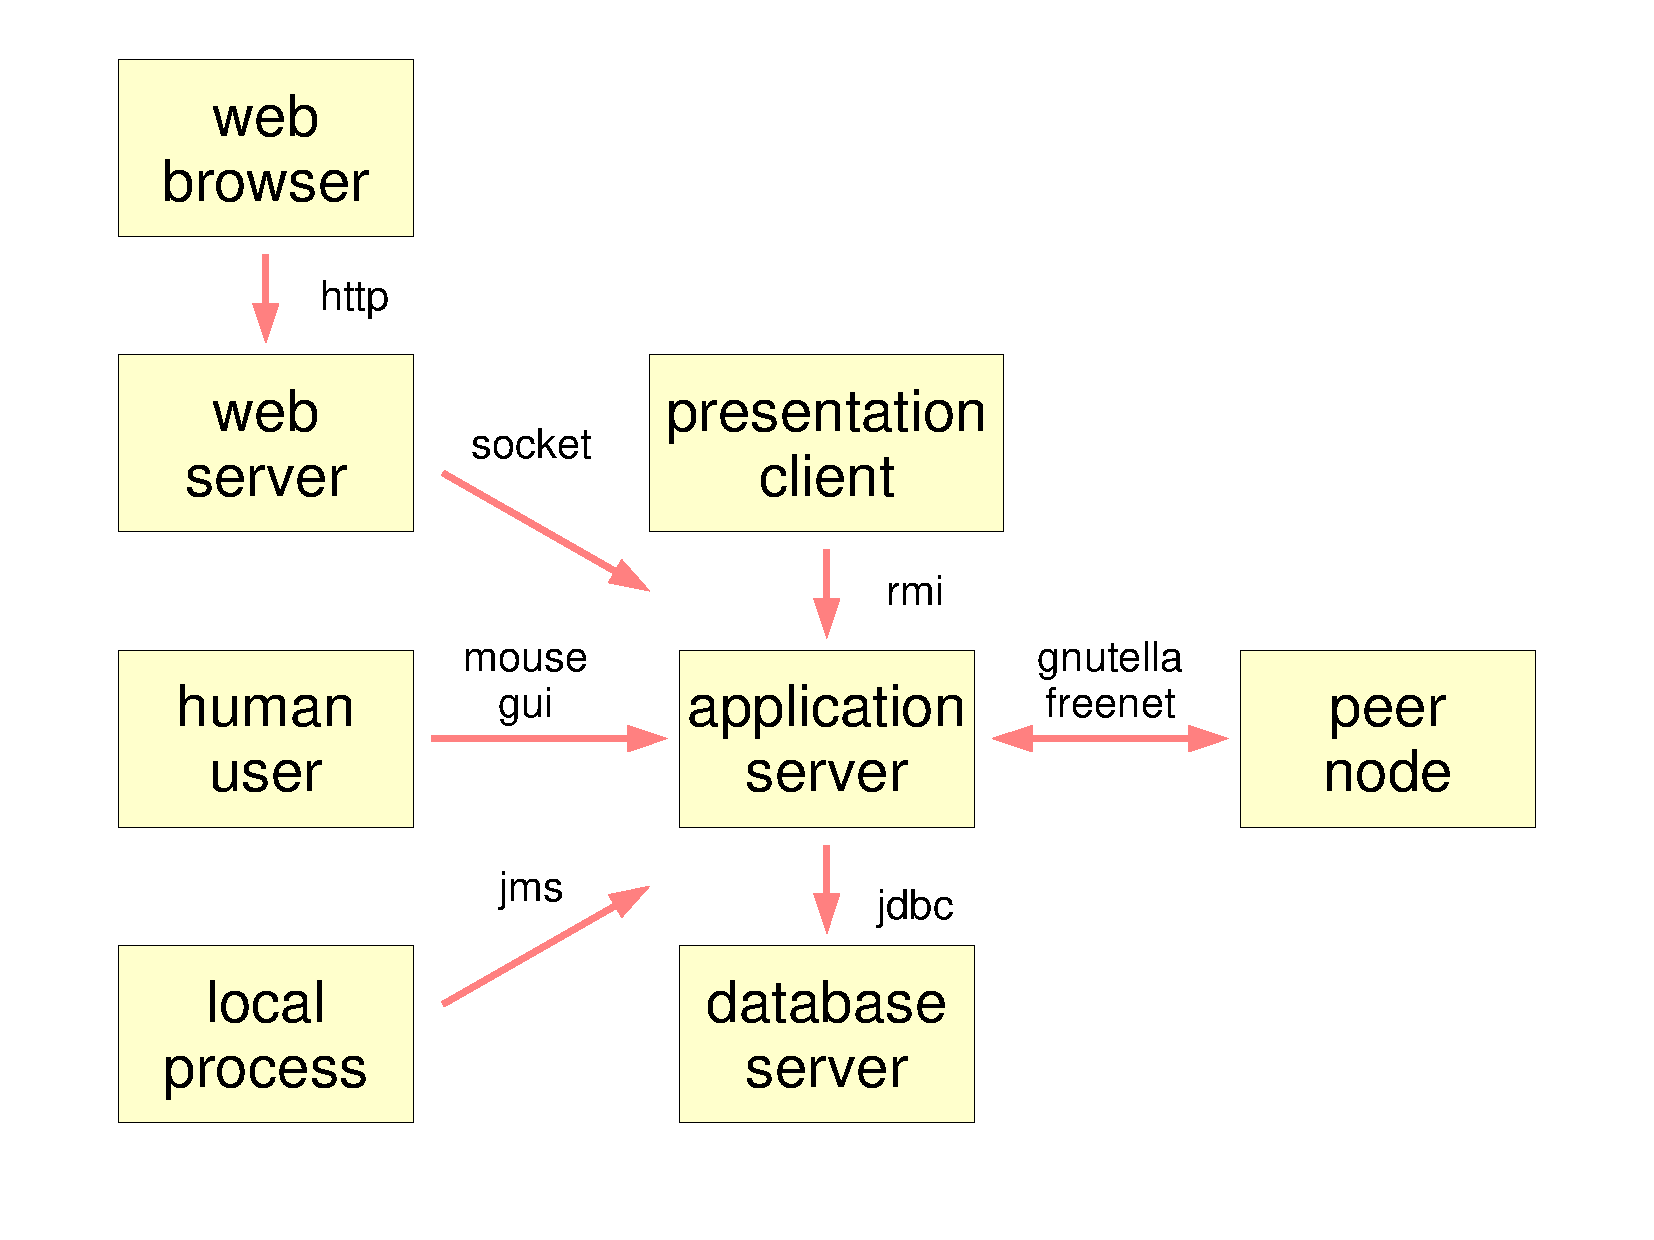
\includegraphics[scale=0.3,angle=-90]{graphic/peer.pdf}
        \caption{Peer-to-Peer Node Communication}
        \label{peer_figure}
    \end{center}
\end{figure}

Besides the previously mentioned client/ server (c/s) environments, so-called
\emph{Peer-to-Peer} (P2P) computer networks latterly became popular. In them,
nodes do not have just one role, but act as client and server at the same time
(figure \ref{peer_figure}), thus sharing their computing power and bandwidth.
Common P2P protocols are: \emph{Freenet}, \emph{Gnutella2}, \emph{BitTorrent},
\emph{eDonkey}, \emph{FastTrack} or \emph{Napster} \cite{wikipedia}. Many more
exist.

Just like nodes in a P2P network, human beings are capable of communicating
both ways, taking the role of a client or server. The organs that are needed to
do so are put into comparison with the corresponding devices of a computer
system, in chapter \ref{state_and_logic_heading}.

%
% $RCSfile: remote_server.tex,v $
%
% Copyright (C) 2002-2008. Christian Heller.
%
% Permission is granted to copy, distribute and/or modify this document
% under the terms of the GNU Free Documentation License, Version 1.1 or
% any later version published by the Free Software Foundation; with no
% Invariant Sections, with no Front-Cover Texts and with no Back-Cover
% Texts. A copy of the license is included in the section entitled
% "GNU Free Documentation License".
%
% http://www.cybop.net
% - Cybernetics Oriented Programming -
%
% http://www.resmedicinae.org
% - Information in Medicine -
%
% Version: $Revision: 1.1 $ $Date: 2008-08-19 20:41:08 $ $Author: christian $
% Authors: Christian Heller <christian.heller@tuxtax.de>
%

\section{Remote Server}
\label{remote_server_heading}
\index{Remote Server}
\index{Streams}
\index{Common Object Request Broker Architecture}
\index{CORBA}
\index{Simple Object Access Protocol}
\index{SOAP}
\index{Network Dynamic Data Exchange}
\index{NetDDE}
\index{Distributed Component Object Model}
\index{DCOM}
\index{COM+}
\index{KParts}
\index{Universal Network Objects}
\index{UNO}

Figure \ref{remote_figure} introduces a \emph{Remote Server} to the illustrated
example environment. It may access a database system -- similarly to the already
existing application server. In this example, however, it just works on simple
local files, using \emph{Streams}.

\begin{figure}[ht]
    \begin{center}
        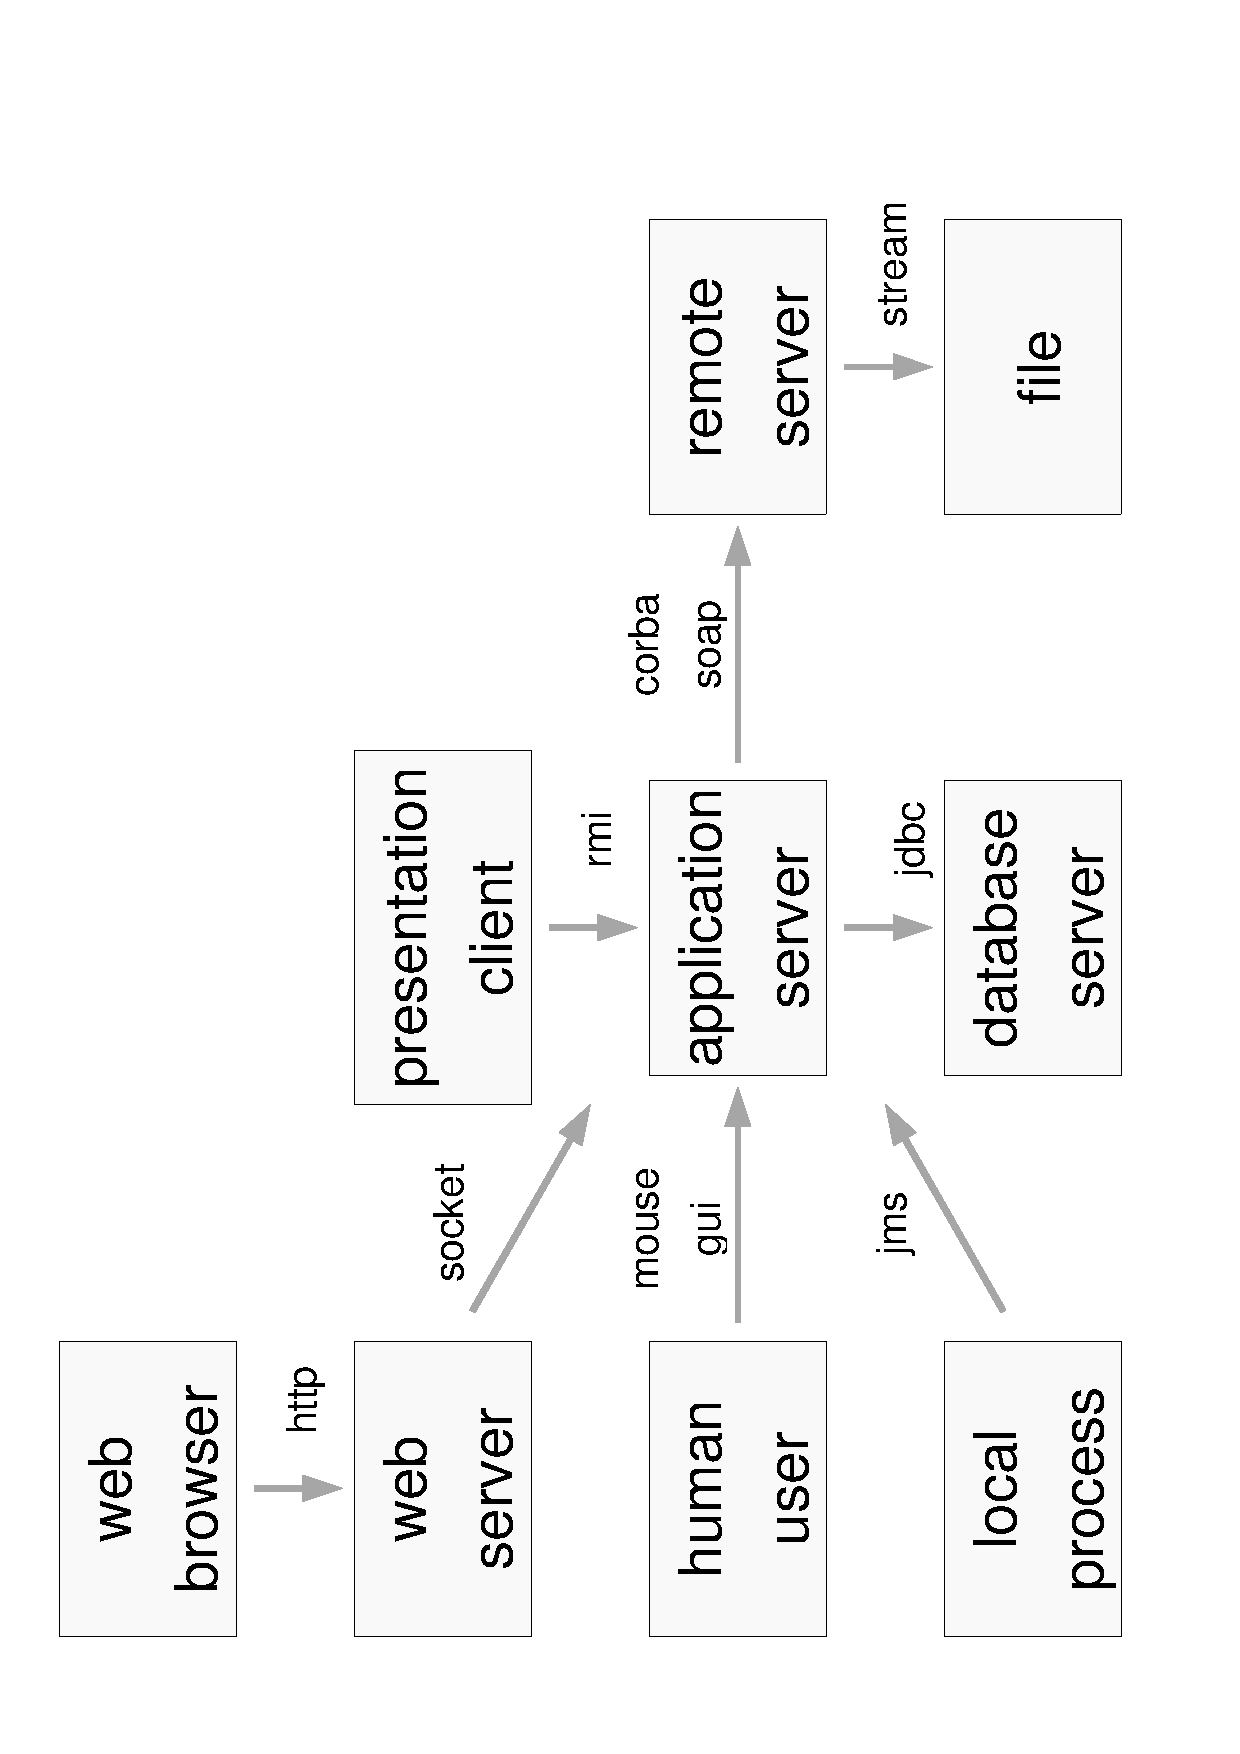
\includegraphics[scale=0.3,angle=-90]{graphic/remote.pdf}
        \caption{Remote Server}
        \label{remote_figure}
    \end{center}
\end{figure}

Like the previously introduced kinds of systems, remote systems need to rely on
a number of standards and mechanisms, in order to be able to communicate over
network. A comparison of some of these is given in \cite{olson, brownech, hrastnik}.
In the following is a list of common techniques that were not yet mentioned
before:

\begin{itemize}
    \item[-] \emph{Common Object Request Broker Architecture} (CORBA)
        \cite{corba, vinoski, gruhn}
    \item[-] \emph{Simple Object Access Protocol} (SOAP) \cite{soap}
    \item[-] \emph{Network Dynamic Data Exchange} (NetDDE) \cite{ddefaq}
    \item[-] \emph{Distributed Component Object Model} (DCOM/ COM+) \cite{gruhn}
    \item[-] \emph{KParts} \cite{kde}
    \item[-] \emph{Universal Network Objects} (UNO) \cite{openoffice}
\end{itemize}

%
% $RCSfile: legacy_host.tex,v $
%
% Copyright (C) 2002-2008. Christian Heller.
%
% Permission is granted to copy, distribute and/or modify this document
% under the terms of the GNU Free Documentation License, Version 1.1 or
% any later version published by the Free Software Foundation; with no
% Invariant Sections, with no Front-Cover Texts and with no Back-Cover
% Texts. A copy of the license is included in the section entitled
% "GNU Free Documentation License".
%
% http://www.cybop.net
% - Cybernetics Oriented Programming -
%
% http://www.resmedicinae.org
% - Information in Medicine -
%
% Version: $Revision: 1.1 $ $Date: 2008-08-19 20:41:07 $ $Author: christian $
% Authors: Christian Heller <christian.heller@tuxtax.de>
%

\section{Legacy Host}
\label{legacy_host_heading}
\index{Legacy Host}
\index{Legacy Systems}
\index{Host}
\index{Mainframe}
\index{Common Business Oriented Language}
\index{COBOL}
\index{Programming Language One}
\index{PL/I}
\index{Virtual Storage Access Method}
\index{VSAM}
\index{Third Party Maintenance}
\index{TPM}
\index{Customer Information Control System}
\index{CICS}

Finally, there is often a need to integrate \emph{Legacy Systems}, which are a
special variant of remote software systems running on computers with an older
architecture. Those computers are also named \emph{Host}, as in the example of
figure \ref{legacy_figure}, or \emph{Mainframe}. The applications running on
them are programmed in languages like the \emph{Common Business Oriented Language}
(COBOL) or \emph{Programming Language One} (PL/I) \cite{pli}, the latter
developed as an \emph{International Business Machines} (IBM) \cite{ibm} product
in the mid 1960's.

\begin{figure}[ht]
    \begin{center}
        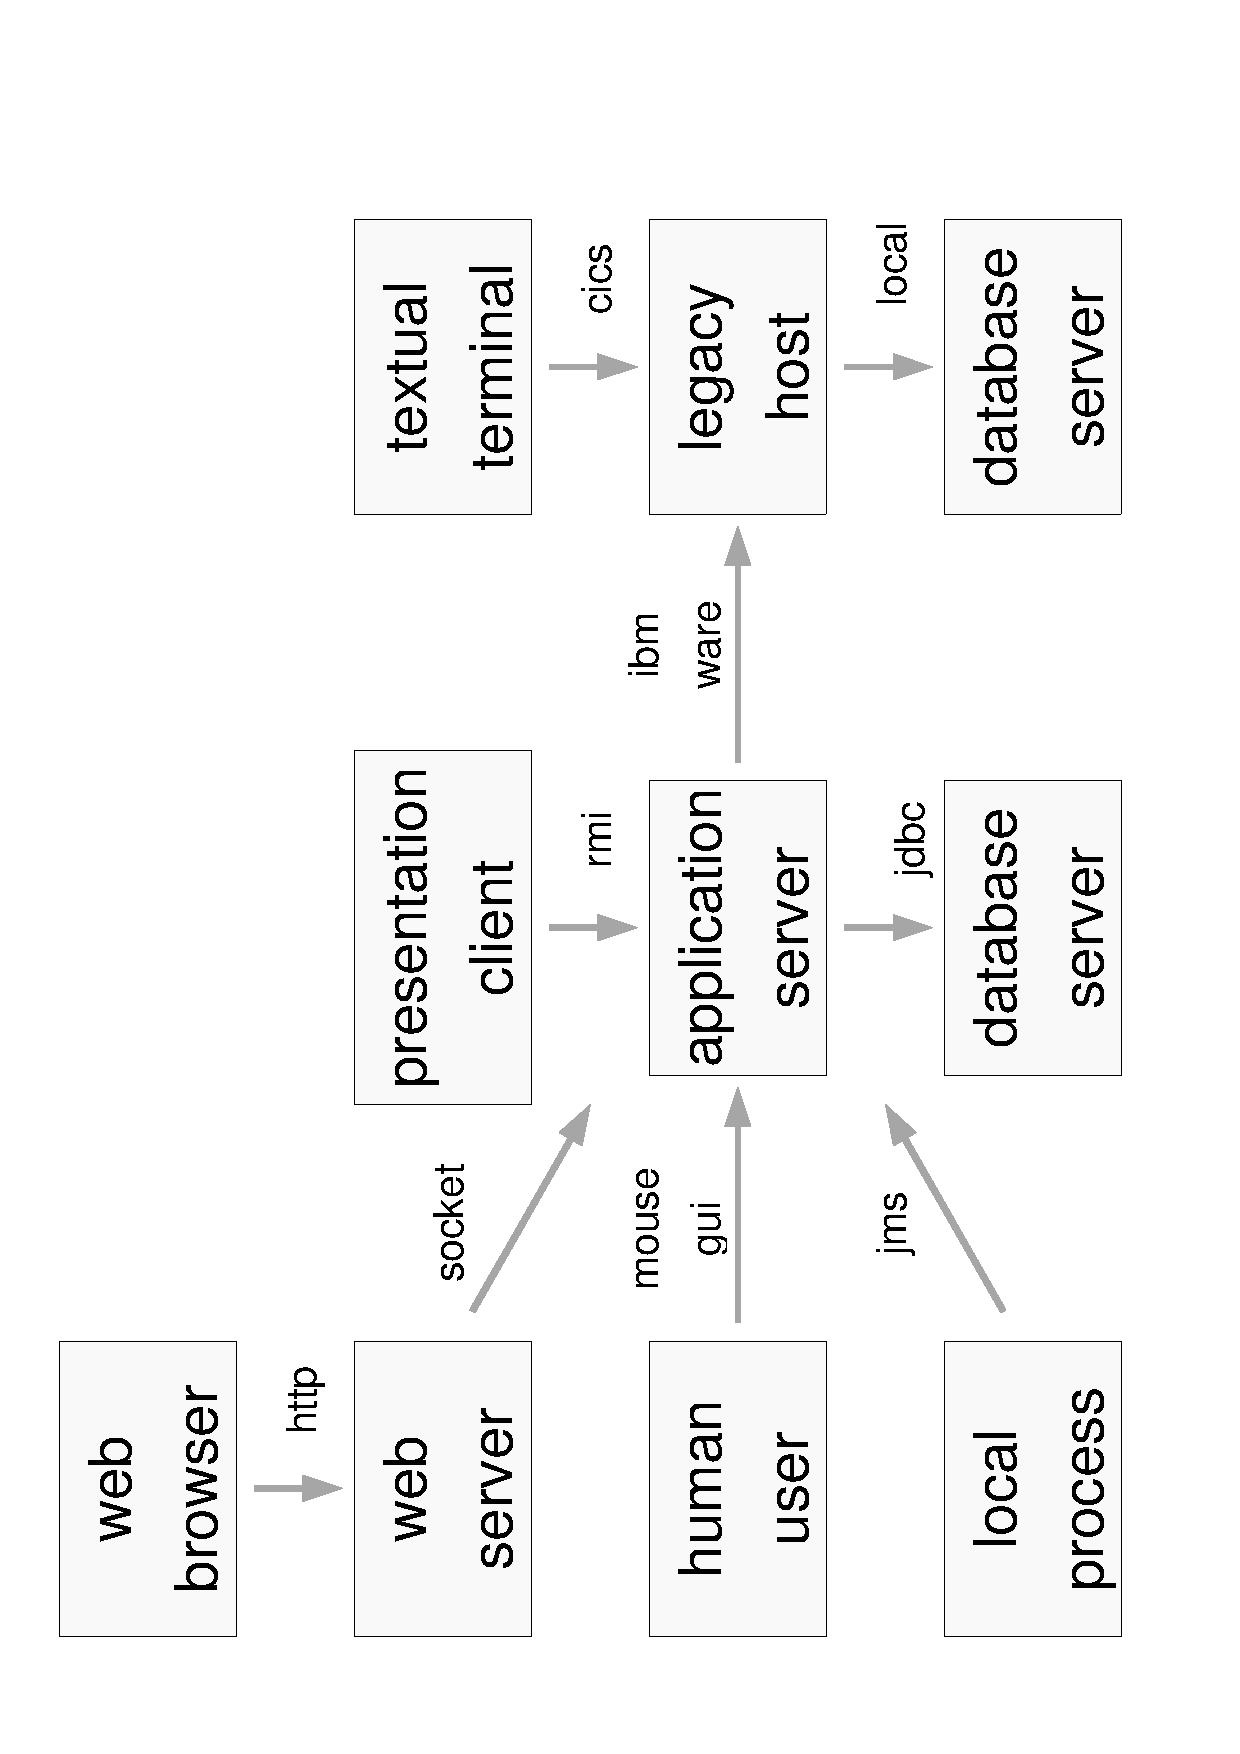
\includegraphics[scale=0.3,angle=-90]{graphic/legacy.pdf}
        \caption{Legacy Host}
        \label{legacy_figure}
    \end{center}
\end{figure}

Host computers manage nearly everything an ancient information technology
environment needs. They are responsible for persistence and processing of data.
Often, they contain hierarchical databases \cite{oolegacysystems} using flat
files like the \emph{Virtual Storage Access Method} (VSAM) format. True clients
do not exist here. Character-based terminals are the way to communicate with
the host which controls all interaction (including keyboard and screen), within
a \emph{Third Party Maintenance} (TPM) \emph{Customer Information Control System}
(CICS) runtime environment.

%
% $RCSfile: systems_interconnection.tex,v $
%
% Copyright (C) 2002-2008. Christian Heller.
%
% Permission is granted to copy, distribute and/or modify this document
% under the terms of the GNU Free Documentation License, Version 1.1 or
% any later version published by the Free Software Foundation; with no
% Invariant Sections, with no Front-Cover Texts and with no Back-Cover
% Texts. A copy of the license is included in the section entitled
% "GNU Free Documentation License".
%
% http://www.cybop.net
% - Cybernetics Oriented Programming -
%
% http://www.resmedicinae.org
% - Information in Medicine -
%
% Version: $Revision: 1.1 $ $Date: 2008-08-19 20:41:09 $ $Author: christian $
% Authors: Christian Heller <christian.heller@tuxtax.de>
%

\section{Systems Interconnection}
\label{systems_interconnection_heading}
\index{Systems Interconnection}
\index{Open Systems Interconnection}
\index{OSI}
\index{International Organization for Standardization}
\index{ISO OSI Reference Model}
\index{Simple Mail Transfer Protocol}
\index{SMTP}
\index{Telephone Network}
\index{Telnet}
\index{File Transfer Protocol}
\index{FTP}
\index{Hypertext Transfer Protocol}
\index{HTTP}
\index{Domain Name Service}
\index{DNS}
\index{X.226}
\index{Remote Procedure Call}
\index{RPC}
\index{Network Basic Input/ Output System}
\index{NetBIOS}
\index{Transfer Control Protocol}
\index{TCP}
\index{User Datagram Protocol}
\index{UDP}
\index{Transport Protocol Class 4}
\index{TP4}
\index{Sequence Package Exchange}
\index{SPX}
\index{Internet Protocol}
\index{IP}
\index{Internet Packet Exchange}
\index{IPX}
\index{Point-to-Point Protocol}
\index{PPP}
\index{Serial Line Internet Protocol}
\index{SLIP}
\index{Frame Relay}
\index{FR}
\index{X.25}
\index{Ethernet}
\index{Token Ring}
\index{Fiber Distributed Data Interface}
\index{FDDI}
\index{Ontology}
\index{Health Level Seven}
\index{HL7}
\index{TCP/IP}
\index{Universal Interactive Executive}
\index{UNIX}
\index{Operating System}
\index{OS}

Communication is essential to an IT environment as described before. To enable
and ease communication across different systems, special solutions have been
developed and accepted as \emph{de facto} or \emph{de jure} standards. One such
specification is the well-known \emph{Open Systems Interconnection} (OSI)
reference model, defined by the \emph{International Organization for Standardization}
(ISO). Numerous books \cite{tanenbaum2000} and documents on the web
\cite{payer} describe this model and its protocols.

\begin{figure}[ht]
    \begin{center}
        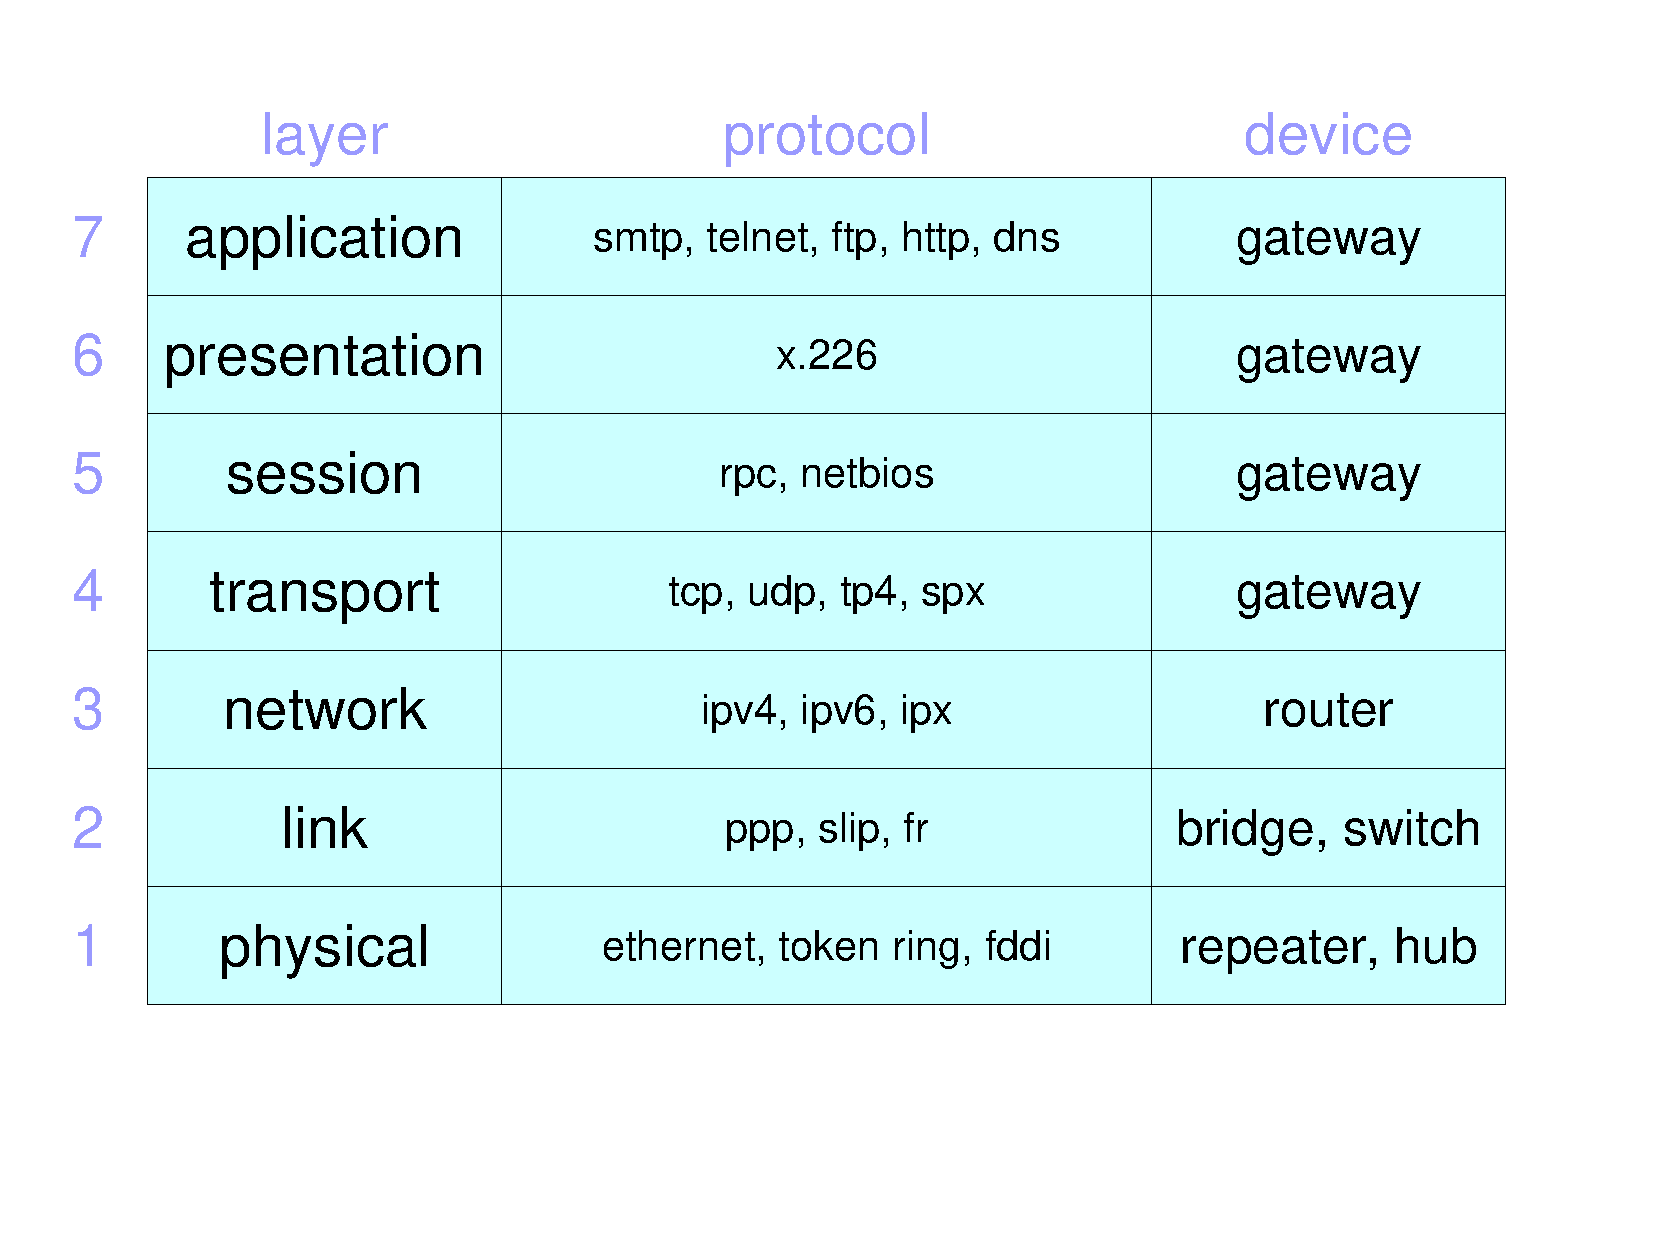
\includegraphics[scale=0.3,angle=-90]{graphic/osi.pdf}
        \caption{ISO OSI Reference Model}
        \label{osi_figure}
    \end{center}
\end{figure}

Figure \ref{osi_figure} organises the seven layers of the model in table form,
with one row representing one layer. The first column contains a layer's name,
the second examples of typical network protocols and the third devices in which
the protocols are used. \emph{Simple Mail Transfer Protocol} (SMTP),
\emph{Telephone Network} (Telnet), \emph{File Transfer Protocol} (FTP),
\emph{Hypertext Transfer Protocol} (HTTP) and \emph{Domain Name Service} (DNS)
are standard protocols used directly in software applications and -tools.
\emph{X.226} is a recommendation defining the OSI presentation protocol. The
\emph{Remote Procedure Call} (RPC) and \emph{Network Basic Input/ Output System}
(NetBIOS) may be sorted into the session layer. \emph{Transfer Control Protocol}
(TCP), \emph{User Datagram Protocol} (UDP), \emph{Transport Protocol Class 4}
(TP4) and \emph{Sequence Package Exchange} (SPX) do belong to the transport
layer. The \emph{Internet Protocol} (IP) is used in two versions: 4 and 6. Both
of them are situated on the network level of the OSI model, just like the
\emph{Internet Packet Exchange} (IPX) protocol. The link level contains the
\emph{Point-to-Point Protocol} (PPP), \emph{Serial Line Internet Protocol}
(SLIP) and \emph{Frame Relay} (FR), the latter being a replacement for veterans
like \emph{X.25}. To the physical level transmitting raw Bits finally, belong
\emph{Ethernet}, \emph{Token Ring} and \emph{Fiber Distributed Data Interface}
(FDDI).

Many of the mentioned protocols may be assigned to more than just one layer.
But it is \emph{not} the intention of this work to deal with such details. The
overall ISO OSI model, however, is mentioned because it is a good example of a
structure whose layers represent increasing levels of abstraction, what will
later in this work be called an \emph{Ontology} (chapters
\ref{logical_architecture_heading} and \ref{knowledge_schema_heading}). Also,
the \emph{Health Level Seven} (HL7) medical standard, which gets introduced in
chapter \ref{res_medicinae_heading}, received its name from referring to OSI's
seventh level -- the application level \cite{rogers}.

While the ISO OSI model defines seven abstract communication layers, the
popular \emph{TCP/IP} model uses solely four. Web communication as described in
section \ref{web_client_and_server_heading} is based on it. Today, TCP/IP has
become the standard in network management systems. A majority of them run the
\emph{Universal Interactive Executive} (UNIX) \emph{Operating System} (OS), of
which TCP/IP is an integral part. Margarete Payer \cite{payer} writes:
\textit{Although the OSI Model is affected with various deficiencies, it is
well suitable for didactic purposes.} Further, she mentions that since some
time, Andrew S. Tanenbaum uses a hybrid model for structuring his standard book
on computer networks \cite{tanenbaum2000}, which sticked to neither OSI nor
TCP/IP.

%
% $RCSfile: scalability.tex,v $
%
% Copyright (C) 2002-2008. Christian Heller.
%
% Permission is granted to copy, distribute and/or modify this document
% under the terms of the GNU Free Documentation License, Version 1.1 or
% any later version published by the Free Software Foundation; with no
% Invariant Sections, with no Front-Cover Texts and with no Back-Cover
% Texts. A copy of the license is included in the section entitled
% "GNU Free Documentation License".
%
% http://www.cybop.net
% - Cybernetics Oriented Programming -
%
% http://www.resmedicinae.org
% - Information in Medicine -
%
% Version: $Revision: 1.1 $ $Date: 2008-08-19 20:41:08 $ $Author: christian $
% Authors: Christian Heller <christian.heller@tuxtax.de>
%

\section{Scalability}
\label{scalability_heading}
\index{Scalability}
\index{Vertical Scaling}
\index{Horizontal Scaling}
\index{Symmetric Multiprocessing}
\index{SMP}
\index{Central Processing Units}
\index{CPU}
\index{Operating System}
\index{OS}
\index{Input/ Output}
\index{i/o}
\index{Reliability, Availability, Serviceability}
\index{RAS}
\index{Clustering}
\index{Vertical System}
\index{Horizontal System}
\index{Large Database}
\index{Web Server}
\index{Transactional Database}
\index{Firewall}
\index{Data Warehouse}
\index{Proxy Server}
\index{Data Mining}
\index{Directories}
\index{Application Server}
\index{High Performance Technical Computing}
\index{HPTC}
\index{Media Streaming}
\index{Extensible Markup Language Processing}
\index{XML}
\index{Java Server Pages Application}
\index{JSP}
\index{Secure Socket Layer}
\index{SSL}
\index{Virtual Private Network}
\index{VPN}
\index{Application Types}
\index{Interconnect}
\index{Loosely-coupled external Interconnect}
\index{Tightly-coupled internal Interconnect}

The previous sections demonstrated that there are many different ways to organise
a distributed information technology environment. The physical distribution of
systems is often a user requirement, either to connect different locations or to
reach better performance by sharing the work load. The degree to which a system
can be distributed to different hardware is often called its \emph{Scalability}.
Two models of scaling can be distinguished: \emph{vertical} and \emph{horizontal}
computing (figure \ref{scaling_figure}), whose key characteristics are only
described briefly here.

\begin{figure}[ht]
    \begin{center}
        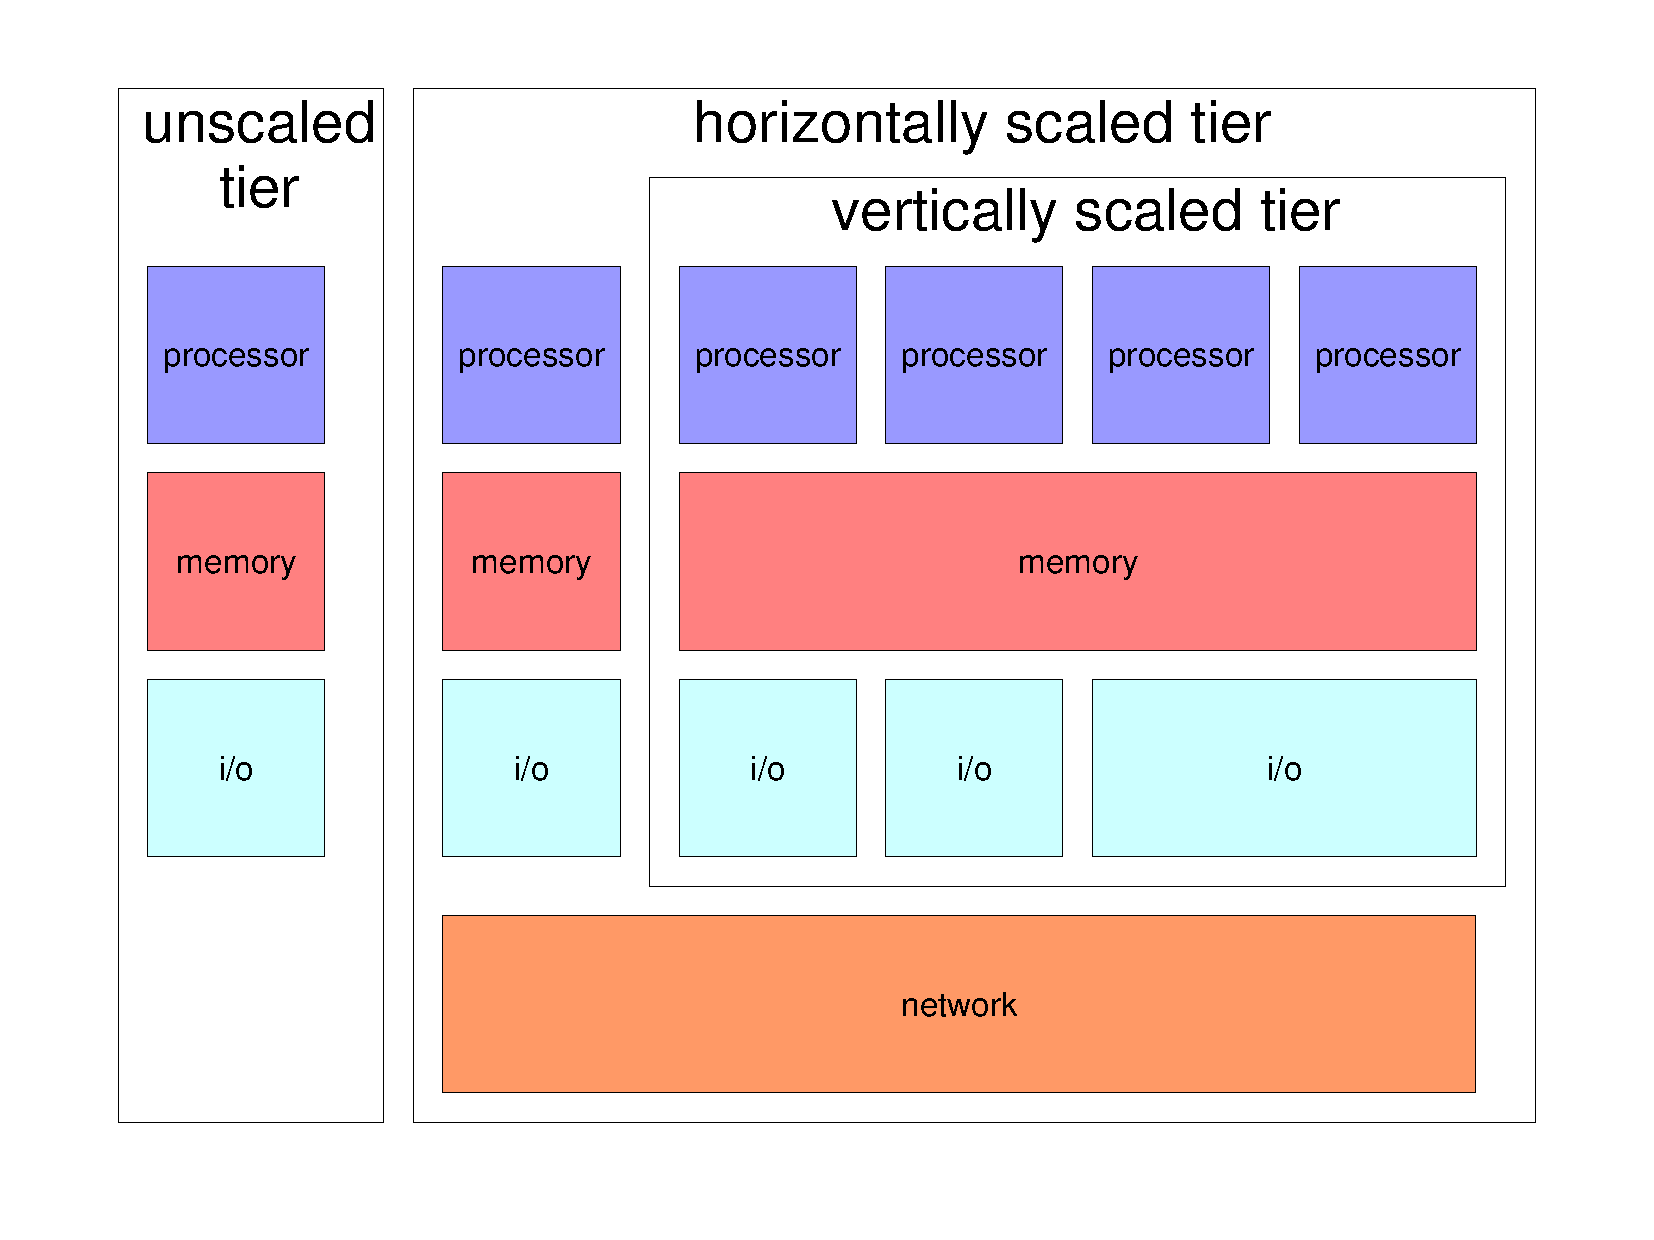
\includegraphics[scale=0.3,angle=-90]{graphic/scaling.pdf}
        \caption{Vertical and Horizontal Scaling}
        \label{scaling_figure}
    \end{center}
\end{figure}

Vertical servers are large \emph{Symmetric Multiprocessing} (SMP) systems with
more than four \emph{Central Processing Units} (CPU) that share one common memory.
One single \emph{Operating System} (OS) instance covers the processors, the memory
and input/ output (i/o) components. Vertical servers provide high availability by
building numerous \emph{Reliability, Availability, Serviceability} (RAS) features
into the individual server, to minimise un-/planned downtime.

The alternative horizontal scaling connects many systems over network, which is
often called \emph{Clustering}. A cluster contains computing nodes having one to
four processors and a memory each. The input/ output devices may belong to just
one node or be shared by many. Each node has an OS instance. \textit{Horizontal
servers do not build RAS features into the individual servers but get high RAS
by replication and deployment of many servers}, as Atwood \cite{atwood} writes.

\begin{table}[ht]
    \begin{center}
        \begin{footnotesize}
        \begin{tabular}{| p{50mm} | p{60mm} |}
            \hline
            \textbf{Vertical System} & \textbf{Horizontal System}\\
            \hline
            Large Database & Web Server\\
            \hline
            Transactional Database & Firewall\\
            \hline
            Data Warehouse & Proxy Server\\
            \hline
            Data Mining & Directories\\
            \hline
            Application Server & Application Server\\
            \hline
            High Performance Technical Computing (HPTC) application (non-partitionable) & High Performance Technical Computing (HPTC) application (partitionable)\\
            \hline
            & Media Streaming\\
            \hline
            & Extensible Markup Language (XML) Processing\\
            \hline
            & Java Server Pages (JSP) Application\\
            \hline
            & Secure Socket Layer (SSL)\\
            \hline
            & Virtual Private Network (VPN)\\
            \hline
        \end{tabular}
        \end{footnotesize}
        \caption{Vertical and Horizontal Application Types \cite{atwood}}
        \label{scalability_table}
    \end{center}
\end{table}

Table \ref{scalability_table} states some typical applications for vertical and
horizontal computing. The key difference, that after \cite{atwood} affected
both, their price and performance, is the \emph{Interconnect} used with each
architecture. Horizontal servers use a loosely-coupled \emph{external}
interconnect. Vertical servers use a tightly-coupled \emph{internal}
interconnect that makes data communications faster.

%
% $RCSfile$
%
% Copyright (c) 2005-2006. Christian Heller. All rights reserved.
%
% Permission is granted to copy, distribute and/or modify this document
% under the terms of the GNU Free Documentation License, Version 1.1 or
% any later version published by the Free Software Foundation; with no
% Invariant Sections, with no Front-Cover Texts and with no Back-Cover
% Texts. A copy of the license is included in the section entitled
% "GNU Free Documentation License".
%
% http://www.cybop.net
% - Cybernetics Oriented Programming -
%
% http://www.resmedicinae.org
% - Information in Medicine -
%
% Version: $Revision$ $Date$ $Author$
% Authors: Christian Heller <christian.heller@tuxtax.de>
%

\subsection{Misleading Tiers}
\label{misleading_tiers_heading}

When distinguishing human- and technical systems, the kinds of
\emph{Communication} are:

\begin{itemize}
    \item[-] Human $\leftrightarrow$ Human
    \item[-] Human $\leftrightarrow$ Computer
    \item[-] Computer $\leftrightarrow$ Computer
\end{itemize}

Each of these relies on different techniques, transport mechanisms, languages
(protocols) and so on. But the general principle after which communication
works, is always the same -- no matter whether technical \emph{Computer}
systems or their biological prototype, the \emph{Human Being}, are considered:
Information is \emph{received}, \emph{stored}, \emph{processed} and \emph{sent}.
Despite these common characteristics, today's \emph{Information Technology}
(IT) environments \cite{hellerkunze} treat communication between a computer
system and a human being differently than that \emph{among} computer systems.

\begin{figure}[ht]
    \begin{center}
        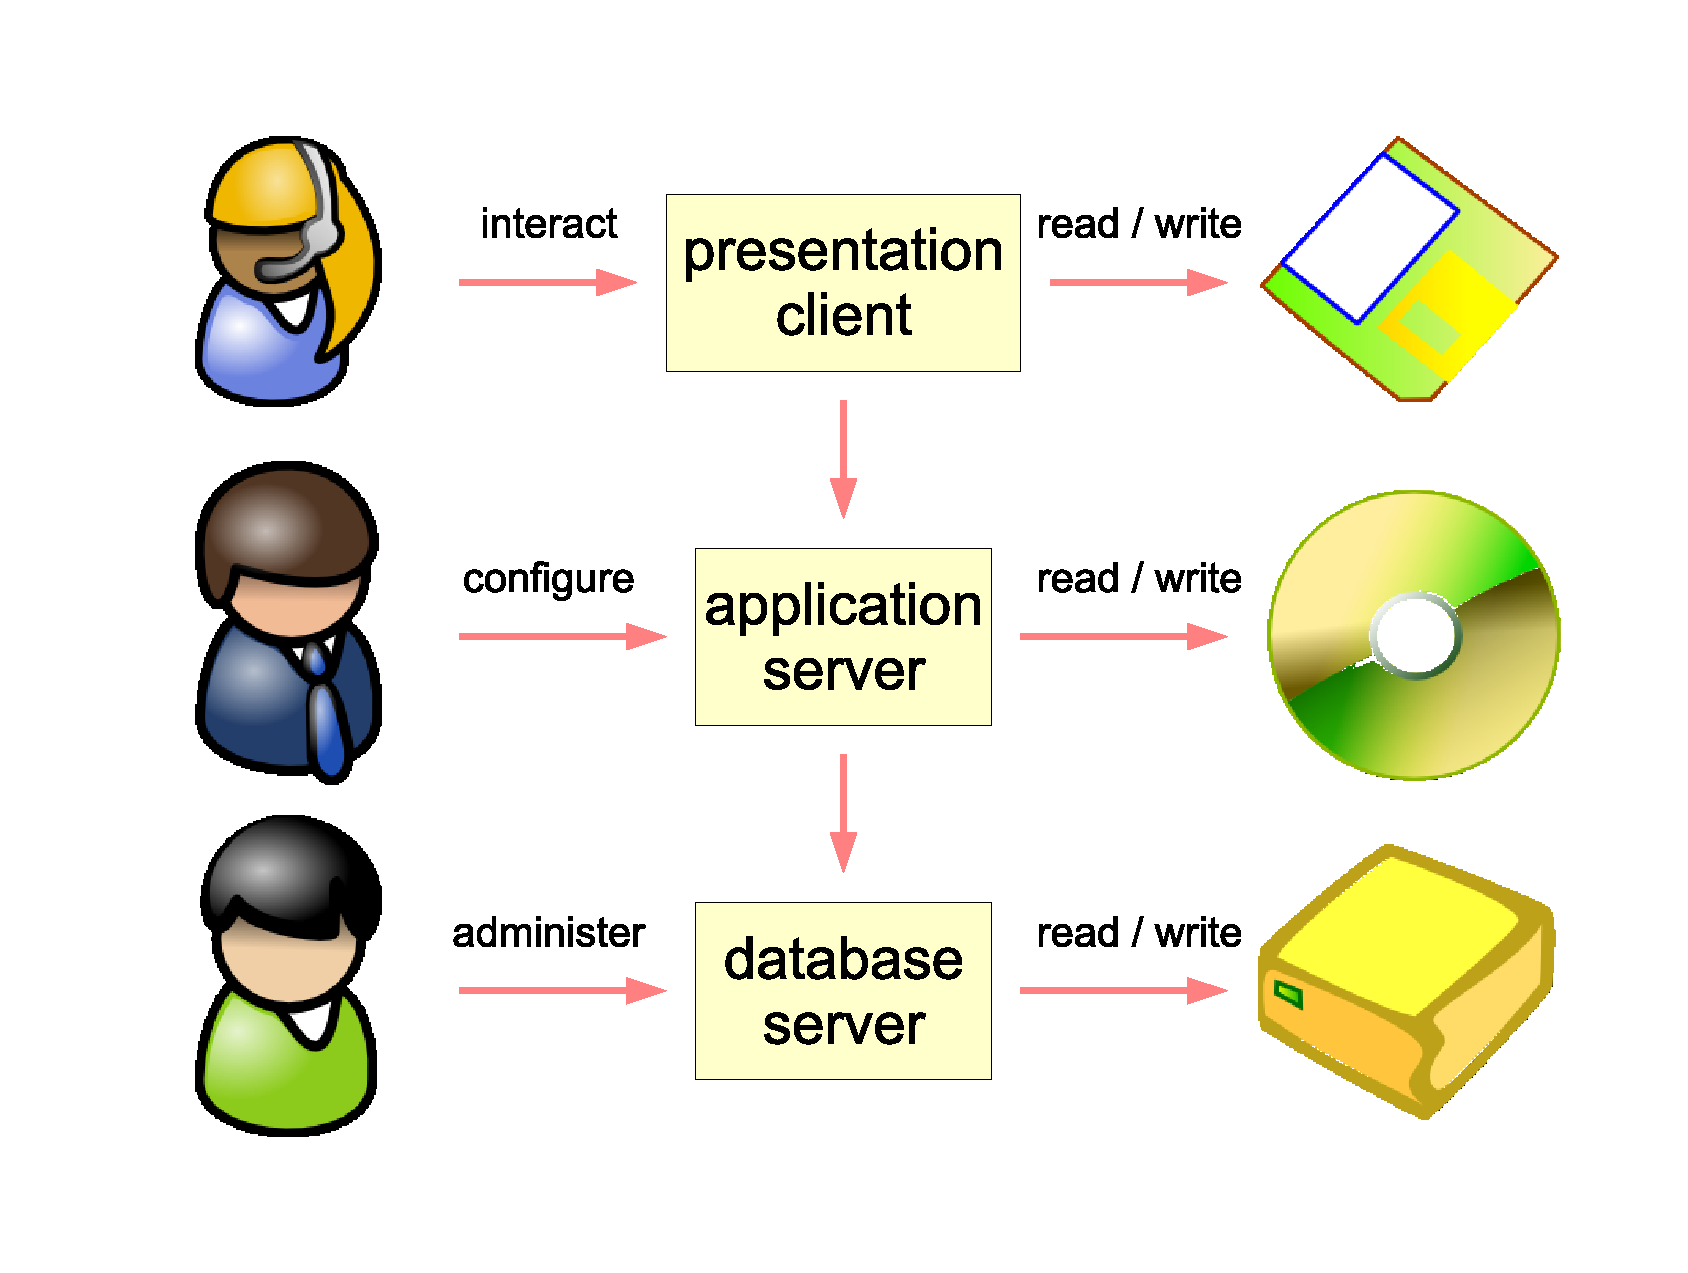
\includegraphics[scale=0.2]{vector/misleading.eps}
        \caption{Universal Communication}
        \label{misleading_figure}
    \end{center}
\end{figure}

Figure \ref{misleading_figure} shows a three-tier environment: tier 1 represents
the \emph{Presentation Layer}; tier 2 stands for the \emph{Application Layer};
tier 3 is the \emph{Database (DB) Layer}. Typical synonyms are, in this order:
\emph{Frontend}, \emph{Business Logic} and \emph{Backend}. The tiers (layers)
serve two needs: connect different locations and share work load (\emph{Scaling}).
However, the split into tiers of that kind raises two illusions:

\begin{enumerate}
    \item \emph{Users only interact with clients}
    \item \emph{Persistent data are stored in DB only}
\end{enumerate}

Many IT architectures, or at least their illustrations, neglect the fact that
in reality \emph{all} systems need a \emph{User Interface} (UI), for at least
being administered by humans, and \emph{almost} all systems, even
\emph{Database Management Systems} (DBMS) themselves, store some of their
persistent data outside a database, for example locally available configuration
information. This is not necessarily a problem for the IT environment as such,
but it is for the internal architecture of software systems. Special solutions
have to deal with frontend (UI framework), business logic (domain patterns) and
backend (data mapping), and often additional mechanisms for local and remote
communication. The serious differences in these design solutions are one root
of well-known problems like multi- directional inter-dependencies between system
parts, that make software difficult to develop and hard to maintain.

One aim of the work described in this article was to investigate possibilities
for a \emph{unification} of communication paradigms, that is high-level design
paradigms rather than low-level protocols, in order to architect software in a
way that allows the computer system it runs on to communicate \emph{universally}.


    %
% $RCSfile: summary.tex,v $
%
% Copyright (c) 2001-2004. Christian Heller. All rights reserved.
%
% No copying, altering, distribution or any other actions concerning this
% document, except after explicit permission by the author!
% At some later point in time, this document is planned to be put under
% the GNU FDL license. For now, _everything_ is _restricted_ by the author.
%
% http://www.cybop.net
% - Cybernetics Oriented Programming -
%
% http://www.resmedicinae.org
% - Information in Medicine -
%
% @author Christian Heller <christian.heller@tuxtax.de>
%

\section{Summary}
\label{summary_heading}

This paper means that wild \emph{Dependencies} are a major reason for error-prone,
unstable, unflexible, unmaintainable software systems. Two facts causing such
dependencies are the \emph{Bundling} of static and dynamic properties by
object-oriented languages and the \emph{Mix} of knowledge and hardware control
in traditional programming languages. This information mix additionally forces
software development projects to run through a course of different abstraction
steps which would not differ if one common knowledge abstraction were used.

As solution to the above's problems, this document suggests to build software
systems after the concepts of \emph{Human Thinking}. The approach, named CYBOP,
such follows the recommendations of the science of \emph{Cybernetics} and its
specialization \emph{Bionics}, whereby biological principles should be applied
to the study and design of engineering systems. An abstract model as formed in the
human mind represents an \emph{Item}, \emph{Category} and \emph{Compound}, at the
same time. Additionally, it contains \emph{Meta Information} about its parts.
This information often corresponds to physical dimensions and determines whether
the model is an abstraction of \emph{static} or \emph{dynamic} real-world aspects.

The introduced \emph{CYBOL} language has the semantics to express knowledge models
as used by human thinking. It allows to create complete application systems. Its
syntax is based on \emph{XML} which results in absolutely platform- independent
system definitions. CYBOL files get interpreted by the \emph{CYBOI} interpreter
and can be changed at runtime. CYBOI manages all hardware access. It concentrates
model instances and signal handling in one place and such avoids memory leaks and
endless loops.

CYBOL models could be displayed graphically, using special design tools. But their
\emph{formal definition} also allows them to be used as main abstraction throughout
all phases in a software project's lifetime. Analysts and experts can start their
work by creating rudimentary CYBOL models (defining static structures and dynamic
processes) which software designers can later complete and check for correctness.
The implementation phase becomes superfluous at all: CYBOL models already represent
the system to be built, no further code is needed! It is hard to imagine the amount
of saved time and costs for software projects. Even better: Experts are placed in
a position to, themselves, actively help creating systems.

    %
% $RCSfile: acknowledgements.tex,v $
%
% Copyright (C) 2002-2008. Christian Heller.
%
% Permission is granted to copy, distribute and/or modify this document
% under the terms of the GNU Free Documentation License, Version 1.1 or
% any later version published by the Free Software Foundation; with no
% Invariant Sections, with no Front-Cover Texts and with no Back-Cover
% Texts. A copy of the license is included in the section entitled
% "GNU Free Documentation License".
%
% http://www.cybop.net
% - Cybernetics Oriented Programming -
%
% http://www.resmedicinae.org
% - Information in Medicine -
%
% Version: $Revision: 1.1 $ $Date: 2008-08-19 20:41:05 $ $Author: christian $
% Authors: Christian Heller <christian.heller@tuxtax.de>
%

\section*{Acknowledgements}
\label{acknowledgements_heading}
%\addcontentsline{toc}{section}{Acknowledgements}

Certainly, first thanks is due my wife \emph{Kasia} and my \emph{Parents} and
\emph{Sisters}, being always with me, in good as in bad times. Not less
important to me are my aunt \emph{Maria Kosiza}, my great \emph{Relatives} and
our former chaplain \emph{Johannes Preis}, who have helped shaping me the way I
am.

I would like to thank my professor, \emph{Ilka Philippow}, for greatly
encouraging me during my work while leaving enough room to develop my own
ideas. Equal thanks is due my supervisors \emph{Dietrich Reschke} and
\emph{Mark Lycett}. \emph{Detlef Streitferdt} and \emph{Bernd D\"ane} gave
numerous hints improving the quality of the first part of my work. Consultation
with Bernd and \emph{Wolfgang Fengler} helped me understand Petri Net diagrams
and their hardware background as well as Assembler programming. Whenever I
got doubts about what I was doing, I was very lucky to receive good motivation
from my colleagues \emph{Volker Langenhan}, \emph{Oswald Kowalski},
\emph{Todor Vangelov} and \emph{Kai B\"ollert}. Oswald's talks about hardware
concepts made me find useful parallels to software. Alexander Fleischer helped
out when I was struggling with \LaTeX's paper size option.

My thanks go to my students \emph{Jens Bohl}, \emph{Torsten Kunze},
\emph{Dirk Behrendt}, \emph{Kumanan Kanagasabapathy}, \emph{Jens Kleinschmidt},
\emph{Martin Fache}, \emph{Karsten Tellhelm}, \emph{Marcel Kiesling},
\emph{Teodora Kikova}, \emph{Dennis Reichenbach}, \emph{Stefan Zeisler},
\emph{Michael Simon}, \emph{Henrik Brandes} and \emph{Saddia Malik} for
contributing their theses, tutorials or source code to the project. Special
thanks to \emph{Rolf Holzm\"uller} who brought in some innovative ideas for
CYBOL, in the final phase of my work, and helped cleaning many bugs in CYBOI.

Reminiscences on good times go to my former colleagues of \emph{OWiS Software}
who, together with the \emph{Technical University of Ilmenau} (TUI), have
contributed with great commitment to the development of the
\emph{Object Technology Workbench} (OTW) UML tool which I would have liked to
use in the early stages of my work. Pity it hasn't gone Open Source after its
development was stopped in 2000 :-( Thanks to \emph{Martin Wolf},
\emph{Rene Prei\ss{}el}, \emph{Dirk Henning} and all colleagues who have been
patient and well-explaining teachers!

I would like to acknowledge the contributors of \emph{CYBOP} \cite{cybop} and
\emph{Res Medicinae} \cite{resmedicinae}, especially all medical doctors, e.g.
\emph{Claudia Neumann} and \emph{Karsten Hilbert}, who supported the second
project with their analysis work \cite{resmedicinae2001} and mailing list
discussions. Furthermore, I want to mention \emph{Thomas Beale} from the
\emph{OpenEHR} project \cite{openehr} whose freely published design document
(back in 2001) gave me some initial ideas in the early stage of my work.
Acknowledged be all these brave \emph{Enthusiasts} of the
\emph{Free/ Libre Open Source Software} (FLOSS) community, who have provided me
with a great amount of knowledge through a comprising code base to build on.
I shall mention the contributors of FLOSS projects such as \emph{Scope}
\cite{scope}, \emph{Apache Jakarta} \cite{jakarta}, \emph{JOS} \cite{jos},
\emph{JDistro} \cite{jdistro}, the \emph{OpenHealth} \cite{openhealth} mailing
list readers, the \emph{OSHCA} \cite{oshca} members and all other supporters of
our projects and ideals.

Great thanks goes to the \emph{Urban und Fischer} publishing company, for
providing anatomical images from their \emph{Sobotta: Atlas der Anatomie}
\cite{urban} and to the \emph{Open Clip Art} project \cite{openclipart} for its
wonderful library of free art! Similarly, I have to thank the free online
dictionaries of \emph{LEO} \cite{leo} and the
\emph{Technical University of Chemnitz} \cite{tuchemnitz}.

I am grateful to all people who openly publish their knowledge on the web.
Without the numerous free sources, I would have never been able to accomplish
this work. Especially in the state-of-the-art part, I had to heavily rely on
existing sources. It is also therefore that I have decided to put my work under
the \emph{GNU FDL} licence \cite{gnulicences}. I would be happy to see large
parts of it copied in \emph{Wikipedia} \cite{wikipedia}!

    \label{references_heading}
    \bibliographystyle{geralpha}
    \bibliography{references}
\end{document}

